%%%%%%%%%%%%%%%%%%%%%%%%%%%%%%%%%%%%%%
% yale_thesis.tex
% Elena Gramellini
% Started: 2017/12/05
%
% A bare, sample template for a Yale PhD thesis using yalephd.cls
%%%%%%%%%%%%%%%%%%%%%%%%%%%%%%%%%%%%%%

\documentclass[letterpaper,12pt]{yalephd}
% remove draft option for final printing.
% font size must be between 10pt-12pt.
\usepackage{caption,setspace}
\usepackage{amsmath} 
\usepackage{rotating}
%\usepackage{newtxtext,newtxmath,amsmath}
\usepackage{ textcomp }


\usepackage{geometry} % you need this for yalephd.cls to work.
\usepackage{graphicx}
\usepackage[graphicx]{realboxes}
 % you probably want the rest of these.
\usepackage{dcolumn}
\usepackage{bm}
\usepackage{hyperref}
\usepackage[export]{adjustbox}

\usepackage{mathtools}
\DeclarePairedDelimiter\bra{\langle}{\rvert}
\DeclarePairedDelimiter\ket{\lvert}{\rangle}
\DeclarePairedDelimiterX\braket[2]{\langle}{\rangle}{#1 \delimsize\vert #2}
\usepackage{textgreek}

\usepackage{multirow}
\usepackage{amsmath}
\usepackage{amsfonts}
\usepackage{amssymb}
\usepackage{appendix}
\usepackage{comment}
\usepackage{cite}
\usepackage{color}
\bibliographystyle{plain}
\usepackage{slashed}  

%\setcounter{chapter}{-1}

\newenvironment{dedication}
  {%\clearpage           % we want a new page          %% I commented this
   \thispagestyle{empty}% no header and footer
   \vspace*{\stretch{1}}% some space at the top
   \itshape             % the text is in italics
   \raggedleft          % flush to the right margin
  }
  {\par % end the paragraph
   \vspace{\stretch{3}} % space at bottom is three times that at the top
   \clearpage           % finish off the page
  }

\usepackage{lineno,xcolor}


%\linenumbers

\begin{document}

% Need to define title before the abstract.
\title{Measurement of ($\pi^-$-Ar) and ($K^+$-Ar) total hadronic cross sections at the LArIAT experiment}
\author{Elena Gramellini}
\advisor{Bonnie T. Fleming}
\date{Date you'll receive your degree} % usually not \today.

% All the stuff at the front of your thesis.
\frontmatter

\begin{abstract}
%Abstract goes here. Limit 750 words.

The Liquid Argon Time Projection Chamber (LArTPC) represents one of the
most advanced experimental technologies for physics at the Intensity
Frontier due to its full 3D-imaging, excellent particle identification
and precise calorimetric energy reconstruction. By deploying a LArTPC in
a dedicated calibration test beam line at Fermilab, LArIAT (Liquid
Argon In A Testbeam) aims to experimentally calibrate this technology
in a controlled environment and to provide physics results key to the
neutrino oscillation physics and proton decay searches of the Short
Baseline Neutrino (SBND, MicroBooNE, ICARUS) and Long Baseline Neutrino programs (DUNE).

LArIAT's physics program entails a vast set of topics with a
particular focus on the study of nuclear effects such as pion and
kaon characteristic interaction modes. 

This thesis presents two world's first measurements: the measurement of ($\pi^-$-Ar) total hadronic cross section in the 100-1050 MeV kinetic energy range and the measurement of the ($K^+$-Ar) total hadronic cross section in the 100-650 MeV kinetic energy range. The analyses devised for these measurements use both the core elements of LArIAT: beamline and LArTPC. The first step in each analysis is the development of an event selection based on  beamline and TPC information geared towards the identification of the hadron of interest. We then proceed to match the beamline candidate to a suitable TPC track. Finally,  we apply the ``thin slice method" technique and measure the cross section, correcting for background contamination and detector effects. The thin slice technique is a new method to measure hadron-argon cross sections possible only due to the combination of the tracking and calorimetry capability of the LArTPC technology. 
Albeit never on argon, the hadronic cross section of pions has been extensively measured before on lighter and heavier different elements in thin target experiments, leading to solid predictions for measurements on argon. Through the use of a different technique, our measurement of the  ($\pi^-$-Ar) total hadronic cross section is in general agreement with the predictions by the Geant4 Bertini Cascade model which are based on data from thin target experiments. On the contrary, cross section measurements for kaons are extremely scarce, thus more difficult to model. Our measurement of the  ($K^+$-Ar) total hadronic cross section is mostly in tension with the Geant4 prediction over the explored range of energies and provides new experimental data to properly compare existing interaction models.

This thesis also reports two  ancillary  detector physics measurements necessary for the cross section analyses: the measurements of the LArIAT electric field and calorimetry constants. We developed a technique to measure the LArIAT electric field using cathode-anode piercing tracks with cosmic data. We applied a new technique for the measurement of the calorimetry calibration constants based on the particles' momentum measurement.


The ($\pi^-$-Ar) and the ($K^+$-Ar) total hadronic cross measurements are the first physics results of the LArIAT experiment and will be the basis for the future LArIAT measurements of pion and kaon cross sections in the exclusive channels.
The outcome of these measurements will ultimately enable to quantify and reduce the systematic associated with the hadronic interaction models in neutrino-argon interactions.

\end{abstract}


\maketitle
\makecopyright{2018}

 \begin{dedication}
A mia mamma e mio babbo,\\
grazie per le radici e grazie per le ali.
    \par   %% or a blank line
    \vspace{2\baselineskip}
To my mom and dad,\\
thank you for the roots and thank you for the wings.
    \vspace{\baselineskip}
  \end{dedication}

\tableofcontents
%\listoffigures % remove this if you have no figures.
%\listoftables % remove this if you have no tables.

\chapter{Acknowledgements} % this needs to be before \mainmatter.

\noindent ``\emph{Dunque io ringrazio tutti quanti.} \hfill ``\emph{So, I thank everyone.} 

\noindent \emph{Specie la mia mamma} \hfill \emph{Especially my mom} 

\noindent \emph{che mi ha fatto cos\'i funky.}" \hfill \emph{who made me so funky.}"

{\raggedleft -- Articolo 31, Tanqi Funky, 1996 -- \par}
\vspace{0.5cm}

%A lot of people are awesome, especially you, since you probably agreed to read this when it was a draft. 


I jumped the pond a little less than 5 years ago because I had a taste of what being a physicists in the US might be like and wanted more.  I came to this vast and sometimes inhospitable land thinking I'd learn a lot of physics (which I did) and hoping I'd keep doing research for as long as I could (which I'm fortunate enough to say I'll still do for a while). Little did I know that getting my PhD would be first and foremost a journey to self discovery, the beginning of a path to asymptotically tend to the person and the scientist I want to be. A journey impossible without the help of many people, which I will now proceed to thank. Let's hope that the acknowledgements won't be longer than the thesis itself.

Mom, you are and will always be the hero of my story; I know this has been challenging for you, thanks for being there for me at every hour of the day and the night, for being always honest and for somehow handling this whole US-Italy thing gracefully. I can't believe you still haven't met Bonnie. Ah, and don't worry, I'll always translate things for you. 

Bonnie Fleming, my advisor, I don't even know where to start in thanking you. Thanks for listening to me before I proved I was worth be listened to; thanks for always believing I could make it, even at the bottom of my doubts; thanks for all the laughters, for all the freedom, for all the great advices; thanks for leading by example; thanks for being always supportive of all my crazy side projects; thanks for choosing each and every person in the most wonderful research group ever and thanks for letting me be part of it. Thanks for showing me that even Bonnie %Freaking 
Fleming is human, has her downs and still she thrives.

Flavio Cavanna, my co-advisor, working with you has been one of the greatest pleasures of my academic life; the extent of your knowledge never ceases to amaze me and the freshness of your enthusiasm is always contagious. Thanks for all the time spent in your office banging our heads on these cross section analyses and thanks for convincing me to join LArIAT in the first place.

Ornella Palamara, after a particularly heated exchange at a wine and cheese, I once told Andrzej I think of you as my spirit animal: fierce, knowledgeable and direct; he replied I still need to walk many miles to get there and I can't agree more.

A big thank you to my academic sisters, from the youngest to the oldest (again academically speaking): Supraja Balasubramanian, you worked the magic of enriching my past, thank you from the bottom of my heart;  Brooke Morrison, the depth of your knowledge, your drive and love for our field has been a constant inspiration;  Ariana  Hackenburg, thanks for keeping me sane for the last four years, if you run for president -- as you should -- remember to delete our Skype chats, love and hugs to you dudette; and last but not least Xiao Luo, Fermilab has given me lots of extraordinary gifts, but no one  bigger than your friendship. 

Jen Raaf and Jonathan Asaadi, these analyses would have not seen the light of day without you. Thanks for your many inputs and for letting your door open to talk about physics and/or my latest paranoia. Thanks for the patience and understanding. And thanks for leading that small experiment with a big heart called LArIAT and all its crazy ponies. Speaking of which, thanks to all my collaborators, especially Irene Nutini, who started the path for the pion analysis, Greg Pulliam, who suffered with me at the end of said path, Dan the Man, Jason, Johnny, Will Fo and Mr Bojangles. A special token of gratitude goes to Roberto Acciarri and Andrzej M. Szelc, you are so much more to me than collaborators and previous car owners, you know you'll always have a home in Chicago (or wherever this job will bring me).

Thanks to the MicroBooNE experiment which has been an incredible learning experience.  I want to thank  Sam Zeller for the countless pieces of advice,  my CRT troopers Martin, David, Rui, Igor and Linda  -- if I know something about hardware it's because of you -- and Kazu and  Kirby, who I shamelessly bothered many times for software help, sushi and coffee.

To all the members of the NPG, thanks for all the laughters and all the wise insights. You're the smartest bunch of idiots I've ever met, I love y'all.

Shany Danieli, Louise Laage and Flor Orosz Hunziker, you're the piece of heart I left in New Haven. Shany, I don't know what made you think I was the cool kid in the group, but I'm so glad you stuck with me. I'm not sure I would have survived my first semester at Yale without you. Your intelligence is matched only by your kindness: you have the rare gift to shine and make others shine with you. Louise, my dear, thanks for always finding the time to listen, for your attuned spirit and for the magnolias. Flor, thanks for welcoming me to the new world with love and providing me with the correct definition of ``America".

Thanks to all the people which helped me make Chicago and Fermilab my new home, in particular David Caratelli,  Mateus Carneiro, Pilar Coloma, Ciaran Hughes, Gordan Krnjaic, Seyda Ipek, Kiel Howe, Adi Ashkenazi and Rob Fine.

To the wonderful people who stayed close even with an ocean in between: la Tasso, Marci, la Bea, la Kittirn, Alvin, la Viola e Brogna, Sighi, la Secchi and the people from the ``La Chiappia Nuova" group, thanks for making me feel like I never left.

Finally, thanks to Anto, my husband, my topo and my adventure companion, cause people might think I'm nice and easy, but you know I'm not... And still, you followed me across half the world and you're here, so that I can never feel alone.


% Starts proper arabic numbering of pages and chapters.
`\chapter{Introduction}\label{ch:-1}

This thesis work concerns the first measurement of the  ($\pi^-$-Ar)  total hadronic cross section  in the 100-1000 MeV  kinetic energy range and the first measurement of the ($K^+$-Ar) total hadronic cross section  in the 100-650 MeV  kinetic energy range. We performed these measurements at the LArIAT experiment,  a small (0.25 ton)  Liquid Argon Time Projection Chamber (LArTPC) on a beam of charged particles at the Fermilab Test Beam Facility.  Albeit particle and nuclear physics have a long history of hadronic cross section measurements, the work outlined in this thesis presents a new methodology -- the ``thin slice method" -- for cross section measurements in argon, possible only thanks to the detection capabilities of the LArTPC technology. The combination of fine-grained tracking and excellent calorimetric information provided by the LArTPC technology  allows to see unprecedented details of particle interactions in argon and, in LArIAT, to measure the kinetic energy of a hadron at each step of the tracking. A renewed interest for precision measurements of hadronic cross sections, particularly in argon, arises from the current  panorama of experimental  particle physics at the intensity frontier.

The discovery of the Higgs boson in 2012 marked the triumph of the Standard Model of Particle Physics; exploring what lays beyond is the real challenge in our field today. 
Since their formulation in 1930, neutrinos have been a source of surprises (and Nobel Prizes) for particle physicists, tiny cracks in our understanding of Nature. In particular, the discovery of neutrino oscillation represents the first evidence of physics Beyond the Standard Model (BSM).  From a theoretical point of view, the field is developing new theories to account for the small but non-zero mass of neutrinos, while trying to remain consistent with the rest of the Standard Model.  From an experimental point of view, we are developing technologies and huge collaborations to probe these theories. As we enter the era of precision measurements of neutrino interaction, neutrinos might hold the key to the next generation of discoveries in particle physics.

Experimentally, precision measurements can be achieved only if the detector technology is able to resolve the fine details of a statistically relevant number of interactions. 
With ``fine details" here we mean the ability to distinguish the many products of the neutrino interaction, such as protons, pions, muons and electrons, and to measure their energy.
Historically,  bubble chamber neutrino detectors were the first revolution in neutrino detection: for example, the spatial resolution of Gargamelle allowed the discovery of neutrino neutral current interaction. Despite the high precision of bubble chambers images, this technology is hard to scale to massive size, making statistical analyses on neutrino interactions almost impossible to perform. To make up for the small neutrino interaction cross section, neutrino experiments moved to very large size, at the expenses of spatial precision. This is the case for the detectors which discovered neutrino oscillation:  both Super-Kamiokande and SNO are massive Cherenkov detectors. With LArTPCs, the field is gaining again bubble-chamber like precision but at massive scales. Following the recommendations of  the latest Particle Physics Project Prioritization Panel  \cite{P5}, the US particle physics panorama is directing a substantial effort towards the exploration of the intensity frontier through the construction of massive LArTPCs. In particular, the near future will see the development of a Short Baseline Neutrino Program (SBN) and long baseline neutrino program  (DUNE), both based on the LArTPC detector technology. The US liquid argon program has the potential to answer many of the fundamental open questions in particle physics today, such as: is there a fourth generation neutrino? is CP violated in the lepton sector? are there any additional symmetries? and, can we find an indication of Grand Unified Theories? 

The SBN program at Fermilab is tasked with conclusively addressing the existence of a fourth neutrino generation in the  $\Delta m^2= \Delta m^2_{14} \sim [0.1 - 10]$ eV$^2$ parameter space. The SBN program entails three surface LArTPCs positioned on the Booster Neutrino Beam at different distances from the neutrino production in oder to fully exploit  the L/E dependence of the oscillation pattern:  SBND (100 m from the decay pipe), MicroBooNE (450 m), and ICARUS (600 m). SBN will also perform an extensive 
program of neutrino cross section measurements, fundamental to abate systematics in the oscillation analyses in both SBN and DUNE.

DUNE has a vast neutrino and non-accelerator physics reach. For what it concerns neutrino physics, oscillation analyses in DUNE have the capability of solving the mass hierarchy and octant problem,  and discovering CP violation in the neutrino sector. Besides its neutrino program, DUNE can open an experimental window on Grand Unified Theories (GUTs). GUTs could potentially answer fundamental questions such as the existence of non-zero neutrino masses and matter-antimatter asymmetry, explaining some ``accidents" in the Standard Models, such as the exact cancellation of the  proton and the electron charge.   Directly probing GUTs at the unification energy scale is impossible by any foreseeable collider experiment. We then need an indirect proof such as baryon number violation, which is predicted by almost every GUT in the form of proton decay, bounded nucleon decay or $n-\bar n$ oscillations on long time-scales. Historically, the main technology used in these searches has been water Cherenkov detectors, with Super-Kamiokande setting all the current experimental limits on the decay lifetimes at the order of $\sim 10 ^{34}$ years. The DUNE far detector and its non-accelerator physics program is a interesting new actor on this stage.  LArTPCs can in fact complement nucleon decay searches in modes where water Cherenkov detectors are less sensitive, especially $p\rightarrow K^+\bar{\nu}$  \cite{Adams:2013qkq}.


Such a diverse physics program speaks to the versatility of the LArTPC technology. LArTPCs provide excellent electron/photon separation \cite{Acciarri:2016sli} lacking in Cherenkov detectors which can be leveraged to abate the photon background from neutral current interactions  in $\nu_e$ searches. LArTPCs also share superb tracking capability with bubble chamber detectors, with several additional benefits. They are electronically read out and self triggered detectors; they provide full 3D-imaging with millimeter resolution, precise calorimetric reconstruction and excellent particle identification. %Plus, female physicists are actually writing code and running experiments, not (only) staring at images \textcolor{red}{-- Too much? --} \cite{2006physics4152G}. 

The amount of information a LArTPC can provide makes these detectors rather complex: a series of dedicated measurements is necessary to obtain meaningful physics results from a LArTPC. The complexity of the LArTPC technology for neutrino detection is due to several reasons. Argon is a fairly heavy element, which means that nuclear effects play an important role in the looks of the interaction topology. For example, pions are one of the main products of neutrino interactions; yet,  since data on charged particle interaction in argon is scarce, neutrino event generators have big uncertainties in the re-scattering simulation of hadrons in argon. %No measurement of hadronic cross sections for pions or kaons is available for argon (yet). 
The amount of details in an LArTPC event is easily  parsed by human eye, but can make automatic event reconstruction rather challenging. Thus, reconstruction algorithms in LArTPC need to be tune to recognize the different topologies of the neutrino interaction products in argon. This is particularly true for pions, since they are an abundant product of the neutrino interactionsl the occurrence of a pion interaction in argon can modify the topology of the neutrino event, causing a misidentification of the neutrino interaction.

The LArIAT \cite{Cavanna:2014iqa} experiment is performing precise cross section measurements of charged particles in argon to bridge this gap of knowledge. 
The LArIAT LArTPC sits on a beam of charged particles at the Fermilab Test Beam Facility; the beam provides charge particles of the type and energy range relevant for neutrino interaction of both SBN and DUNE. The ($\pi^-$-Ar) hadronic cross section is a fundamental input for neutrino detectors in liquid argon, as pion interactions can modify the topology and energy reconstruction of neutrino events in the GeV range, where pion production is abundant. The  ($K^+$-Ar) total hadronic differential cross section in LArIAT is particularly relevant for a high identification efficiency in the context of proton decay searches in DUNE in the  $p\rightarrow K^+\bar{\nu}$  channel. In fact, the kaon-argon cross section affects the kaon topology by modifying the kaon tracking and energy reconstruction, impacting the basis for kaon identification in a LArTPC.  
The cross section analyses exploit the totality of LArIAT's experimental handles; they rely on beam line detector information as well as both calorimetry and tracking in the TPC. These analyses are LArIAT's first physics results. 
In order to measure total hadronic  argon cross sections, several steps are necessary. The analysis starts by identifying a sample of the hadron of interest in the beam line and assessing the beam line contaminations. It proceeds with tracking the hadron candidates in the TPC and measuring their calorimetry at each point in the tracking: the fine sampling of an hadron in the TPC forms the set of ``incident" hadrons.  Then, the hadronic interaction point is identified and the raw cross section is calculated. Two correction\\

This body of work is divided in 8 chapters.
We provide a description of the theoretical framework for the measurements in  Chapter \ref{ch:TheTheory}. Chapter \ref{ch:2} outlines the LArTPC detector technology, while
Chapter \ref{sec:experimentDescription} describes LArIAT experimental setup. We present the event selection for both the pion and kaon analyses, as well as the ``thin-slice method" in Chapter \ref{ch:Interactions}.  Chapter \ref{ch:samples}  describes the work done on the data and Monte Carlo samples in preparation of the cross section analyses.
Chapter \ref{ch:PionXS} shows  the results for the ($\pi^-$-Ar) total hadronic cross section measurement. Chapter \ref{ch:KaonXS} shows  the results for the ($K^+$-Ar) total hadronic cross section measurement. We draw the final remarks on this work in Chapter \ref{ch:Conclusions}

A series of additional studies and calibrations were necessary to perform the cross section analyses. Appendix \ref{ch:AppendixB} shows a measurement of the LArIAT LArTPC electric field using cosmic data. Appendix \ref{ch:AppendixB} shows an optimization of the tracking algorithms geared towards maximizing the efficiency of finding the hadronic interaction point. Appendix \ref{ch:AppendixB} shows the calorimetry calibration of the LArIAT LArTPC, which is a pivotal measurement to enable any physics analysis with TPC data.  



\mainmatter
% Have someone read this chapter
% Add citations
  % Wu experiment (parity violation)
  %Super Kamiokande, MINOS
  %No$\nu$a, MACRO 
  %SNO,Gallex,
  %SAGE,  KamLAND 
  % DAYA  Bay,   RENO
% Red stuff!

\chapter{The theoretical framework}

\section{The Standard Model}
The Standard Model (SM) of particle physics is the most accurate theoretical description of the subatomic world and, in general, one of the most precisely tested theories in the history of physics.  The SM describes the strong, electromagnetic and weak interactions among  elementary particles in the framework of quantum field theory, accounting for the unification of electromagnetic and weak interactions for energies above the  vacuum expectation value of the Higgs field. The SM does not describe gravity or general relativity.

The Standard Model is a gauge theory based on the local group of symmetry
\begin{equation}
G_{SM} = SU(3)_C  \otimes SU(2)_T \otimes U(1)_Y
\label{eq:SMGroup}
\end{equation}

where the subscripts indicate the conserved charges: the strong charge, or color C, the weak isospin T (or rather its third component T3) and the hypercharge Y. These quantities can be related to the electric charge Q through the Gell-Mann-Nishijima relation:
\begin{equation}
Q = \frac{Y}{2} + T_3.
\end{equation}

In the quantum field framework, the elementary particles correspond to the irreducible representations of the G$_{SM}$ symmetry group. In particular, the particles are divided in two categories, fermions and bosons, according to their spin-statistics. Described by the Fermi-Dirac statistics, fermions have half-integer spin and are sometimes called ``matter-particles". Bosons or ``force carriers" have integer spin, follow the Bose-Einstein statistics and mediate the interaction between fermions. The fundamental fermions and their quantum numbers are listed in Tab \ref{tab:SMParticles}.

\begin{table}[]
\centering
\begin{tabular}{|cccc|c|c|c|}\hline
Generation               & I                   & II                  & III                 & T                       & Y                   & Q                   \\\hline

\multirow{6}{*}{Leptons}                          &                     &                     &                     &                         &                     &                     \\
& $\begin{pmatrix}\ \nu_e\\ e \end{pmatrix}_L$ & $\begin{pmatrix}\ \nu_\mu\\ \mu \end{pmatrix}_L$ & $\begin{pmatrix}\ \nu_\tau\\ \tau \end{pmatrix}_L$ & $\begin{matrix}\ 1/2\\ -1/2 \end{matrix}$ & $\begin{matrix}\ -1\\ -1 \end{matrix}$ & $\begin{matrix}\ 0\\ -1 \end{matrix}$ \\
                         &                     &                     &                     &                         &                     &                     \\
                         & $e_R$         & $\mu_R$      & $\tau_R$                  & 0                      & -2                  & 1    \\
                         &                     &                     &                     &                         &                     &                     \\\hline
\multirow{7}{*}{Quarks} 
                         &                     &                     &                     &                         &                     &                     \\
& $\begin{pmatrix}\ u\\ d' \end{pmatrix}_L$ & $\begin{pmatrix}\ c\\ s' \end{pmatrix}_L$ & $\begin{pmatrix}\ t\\ b' \end{pmatrix}_L$ & $\begin{matrix}\ 1/2\\ -1/2 \end{matrix}$ & $\begin{matrix}\ 1/3\\ 1/3 \end{matrix}$ & $\begin{matrix}\ 2/3\\ -1/3 \end{matrix}$ \\
                         &                     &                     &                     &                         &                     &                     \\
& $\begin{matrix}\ u_R\\ d'_R \end{matrix}$ & $\begin{matrix}\ c_R\\ s'_R \end{matrix}$ & $\begin{matrix}\ t_R\\ b'_R \end{matrix}$ & $\begin{matrix}\ 0\\ 0 \end{matrix}$ & $\begin{matrix}\ 4/3\\ -2/3 \end{matrix}$ & $\begin{matrix}\ 2/3\\ -1/3 \end{matrix}$ \\
                         &                     &                     &                     &                         &                     &                    \\\hline
\end{tabular}
\caption{SM elementary fermions. The subscripts L and R indicate respectively the negative helicity (left-handed) and the positive helicity (right-handed).}
\label{tab:SMParticles}
\end{table}

Quarks can interact via all three the fundamental forces; they are triplets of SU(3)$_C$, that is they can exist in three different colors: C = R, G, B. If one chooses a base where $u$, $c$ and $t$ quarks are simultaneously eigenstates of both the strong and the weak interactions, the remaining eigenstates are usually written as $d$, $s$ and $b$ for the strong interaction and $d'$, $s'$ and $b'$ for the weak interaction, because the latter ones are the result of a Cabibbo rotation on the first ones.
Charged leptons interact via the weak and the electromagnetic forces, while neutrinos only interact via the weak force. 
The gauge group univocally determines the number of gauge bosons that carry the interaction; the gauge bosons correspond to the generators of the group: eight gluons (g) for the strong interaction, one photon ($\gamma$) and three bosons (W$^\pm$, Z$^0$) for the electroweak interaction.
A gauge theory by itself can not provide a description of massive particles, but it is experimentally well know that most of the elementary particles have non-zero masses. The introduction of massive fields in the Standard Model lagrangian would make the theory non-renormalizable, and - so far - mathematically impossible to handle. This problem is solved in the Standard Model by the introduction of a scalar iso-doublet $\Phi(x)$, the Higgs field, which gives mass to W$^\pm$ and Z$^0$ gauge bosons through the electroweak symmetry breaking and to the fermions through Yukawa coupling \cite{Higgs1964,Higgs19642}.  The discovery of the Higgs boson in 2012 by the LHC experiments \cite{201230,Aad2012} marked the ultimate confirmation  of a long history of Standard Model successful predictions.

\section{Neutrinos:  tiny cracks in the Standard Model}
\subsection{Neutrinos in the Standard Model}
Neutrino were introduced in the SM as left-handed massless Weyl spinors.
The Dirac equation of motion
\begin{equation}
(i\gamma^ \mu \partial_\mu - m) \psi = 0
\end{equation}
for a fermionic field 
\begin{equation}
 \psi =  \psi_L +  \psi_R
\end{equation}
is equivalent to the equaitons
\begin{equation}
i\gamma^ \mu \partial_\mu  \psi_L = m \psi_R
\end{equation}
\begin{equation}
i\gamma^ \mu \partial_\mu  \psi_R = m \psi_L
\end{equation}

for the chiral fields $\psi_R$ and $\psi_L$, whose evolution in space and time is coupled through the mass $m$.
If the fermion is massless, the chiral fields decouple and the fermion can be described by a single Weyl spinor with two independent components~\cite{Weyl:10.2307}. Pauli initially rejected the description of a physical particle through a single Weyl spinor because of its implication of parity violation. In fact, since the spatial inversion operator throws $\psi_R \leftrightarrow \psi_L$, parity is conserved only if the both the chiral components exist at the same time.  For the neutrino introduction in the SM, experiments came in help of the theoretical description.  The constraint of parity conservation weakened after Wu's experiment in 1957 \cite{PhysRev.105.1413}. Additionally,  there was no experimental indication for massive neutrinos nor evidence of interaction via the neutrino right-handed component.% neutrinos likely interacted only via the left-handed component. 

The symmetry group $SU(2)_T \otimes U(1)_Y$ is the only group relevant for neutrino interactions. The SM electroweak lagrangian is the most general renormalizable lagrangian invariant under the local symmetry group $SU(2)_T \otimes U(1)_Y$. The lagrangian couples the weak isotopic spin doublets and singlets described in \ref{tab:SMParticles} with the gauge bosons  $A^{\mu}_{a}$ ($a$ $=$ 1,2,3) and $B^{\mu}$, and Higgs doublet $\Phi(x)$:

\begin{eqnarray}
\lefteqn{\mathcal{L} = i\sum_{\alpha=e,\mu,\tau} \bar{L}'_{\alpha L}  \slashed D L'_{\alpha L} + 
 i\sum_{\alpha=1,2,3} \bar{Q}'_{\alpha L}  \slashed D Q'_{\alpha L} {}}
 \nonumber\\
 & & {} + i\sum_{\alpha=e,\mu,\tau} \bar{l}'_{\alpha R}  \slashed D l'_{\alpha R} + i\sum_{\alpha=d,s,b} \bar{q}'^D_{\alpha R}  \slashed D q'^D_{\alpha R} + i\sum_{\alpha=u,c,t} \bar{q}'^U_{\alpha R}  \slashed D q'^U_{\alpha R}
 \nonumber\\
 & & {} -\frac{1}{4}A_{\mu \nu}A^{\mu \nu} - \frac{1}{4}B_{\mu \nu}B^{\mu \nu}
 \nonumber\\
 & & {} +(D_{\rho}\Phi)^\dagger(D^{\rho}\Phi) - \mu^2\Phi^\dagger\Phi - \lambda(\Phi^\dagger\Phi)^2 
 \nonumber\\
 & & {} -\sum_{\alpha,\beta=e,\mu,\tau} \Big(Y'^l_{\alpha\beta}\bar{L}'_{\alpha L}  \Phi l'_{\beta R} + Y'^{l*}_{\alpha\beta}\bar{l}'_{\beta R}  \Phi^\dagger L'_{\alpha L}\Big)
  \nonumber\\
 & & {} -\sum_{\alpha=1,2,3} \sum_{\beta=d,s,b} \Big(Y'^D_{\alpha\beta}\bar{Q}'_{\alpha L}  \Phi q'^D_{\beta R} + Y'^{D*}_{\alpha\beta}\bar{q}'^D_{\beta R}  \Phi^\dagger Q'_{\alpha L}\Big)
  \nonumber\\
 & & {} -\sum_{\alpha=1,2,3} \sum_{\beta=u,c,t} \Big(Y'^U_{\alpha\beta}\bar{Q}'_{\alpha L}   \widetilde{\Phi} q'^U_{\beta R} + Y'^{U*}_{\alpha\beta}\bar{q}'^U_{\beta R} \widetilde{\Phi}^\dagger Q'_{\alpha L}\Big).
\end{eqnarray}

The first two lines of the lagrangian summarize the kinetic terms for the fermionic fields and their coupling to the gauge bosons $A^{\mu\nu}_a$, $B^{\mu\nu}$ \footnote{In gauge theories the ordinary derivative $\partial_\mu$  is substitued with the covariant derivative $D_\mu$. Here $D_\mu = \partial_\mu + igA_\mu \cdot I + ig'B_\mu\frac{Y}{2}$, where I and Y are the SU(2)$_L$ and U(1)$_Y$ generators, respectively.}.
The third line describes the kinetic terms and the self-coupling terms of the gauge bosons. The forth line is the Higgs lagrangian, which results in the spontaneous symmetry breaking. The last three lines describe the Yukawa coupling between fermions and the Higgs field, origin of the fermion's mass.

The coupling between left-handed and right-handed field generates the mass term for fermions. The SM assumes only left-handed components for neutrinos, thus implying zero neutrino mass. Since any linear combination of massless fields results in a massless field, the flavor eigenstates are identical to the mass eigenstates in the SM.

\subsection{Neutrino Oscillations}
The determination of the flavor of a neutrino dynamically arises from the corresponding charged lepton associated in a change current interaction; for example, a $\nu_e$ is a neutrino which produces an $e^-$, a $\bar\nu_\mu$ is a neutrino which produces a $\mu^+$, $etc$. 
The neutrino flavor eigenstates $\ket{\nu_\alpha}$,  with $\alpha = e,\mu,\tau$, are orthogonal to each other and form a base for the the weak interaction matrix.

Overwhelming experimental data show neutrinos change flavor during their propagation~\cite{Patrignani:2016xqp}. This phenomenon, called ``neutrino oscillations",  was predicted first by Bruno Pontecorvo in 1957 ~\cite{Pontecorvo:1967fh}.  Neutrino oscillations are possible only if the neutrino flavor eigenstate are not identical to the mass eigenstates, thus resulting in the first evidence of physics beyond the Standard Model.  A minimal extension of the Standard Model introduces three mass eigenstates, $\ket{\nu_i}$ ($i = 1,2, 3$), whose mass $m_i$ is well defined. 
The unitary Pontecorvo-Maki-Nakagawa-Sakata matrix transforms the spinor wave functions ($\psi$) of each component  between flavor and mass bases as follows

\begin{equation} 
\sum \psi_\alpha \ket{\nu_\alpha} =  \sum \psi_i \ket{\nu_i}, \rightarrow \psi_\alpha =  U_{PMNS} \psi_i, 
\end{equation}

with

\begin{equation}
U_{PMNS}=\\
\left[ 
\begin{array}{ccc}
c_{12} & s_{12} & 0\\
-s_{12} & c_{12} & 0\\
0 & 0 & 1\\
\end{array}
\right]
\left[ 
\begin{array}{ccc}
c_{13} & 0 &s_{13}e^{-i\delta} \\
0 & 1 & 0\\
-s_{13}e^{-i\delta}& 0 & c_{13}\\
\end{array}
\right]
\left[
\begin{array}{ccc}
1 & 0 & 0\\
0 & c_{23} & s_{23} \\
0& -s_{23} & c_{23} \\
\end{array}
\right]
\left[ 
\begin{array}{ccc}
e^{i\alpha_1} & 0 & 0\\
0& e^{i\alpha_2} & 0\\
0 & 0 & 1\\
\end{array}
\right]
\label{eq:PMNS}
\end{equation}





where $c$ e $s$ stand respectively for cosine and sine of the corresponding  mixing angles ($\theta_{12}$, $\theta_{23}$ and $\theta_{13}$), $\delta$ �is the Dirac CP violation phase, $\alpha_1$ and $\alpha_{2}$   is the eventual Majorana CP violation phases.  Experimental results on neutrino oscillations are generally reported in terms of the mixing angles and of the squared mass splitting $\Delta m^2_{ab} = m^2_{a} - m^2_{b}$, where $a$ and $b$ represent the mass eigenstates. A summary of the current status of experimental results, albeit partial, is given in table \ref{tab:nuosc}.


\begin{table}[htpb]
\centering
\caption{Summary of experimental results on neutrino oscillation parameters. \textcolor{red}{ADD CITATIONS}}
\label{tab:nuosc}
\begin{tabular}{|r|c|c|c|}
\hline
        & Value   & Precision & Experiment \\
\hline
$\theta_{23}$            & 45$^\circ$                      & 9.0\%   & Super Kamiokande, MINOS,\\
$\Delta m^2_{23}$    & 2.5 $10^{-3}$ eV$^2$   & 1.8\% &  No$\nu$a, MACRO \\
\hline
$\theta_{12}$            & 34$^\circ$                     & 5.8\% &  SNO,Gallex,\\
$\Delta m^2_{12}$    & 7.4 $10^{-5}$ eV$^2$   & 2.8\% &  SAGE,  KamLAND \\
\hline
$\theta_{13}$            &   9$^\circ$                    & 4.7\%  & DAYA  Bay, \\
$\Delta m^2_{13}$    & 2.5 $10^{-3}$ eV$^2$   & 1.8\% &  RENO\\
\hline
\end{tabular}
\end{table}

\subsection{Why so sneaky? Neutrino Cross Section Challenge}


\section{Beyond the Standard Model}
The discovery of neutrino oscillation and its implication of non-zero neutrino mass mark  the beginning of a new, exciting era in neutrino physics: the era of physics Beyond the Standard Model (BSM) in the neutrino sector.
We are currently searching for new, deeper theories that can accommodate neutrinos with tiny but non-zero mass, while remaining consistent with the rest of the Standard Model. 

\subsection{Open Questions in Neutrino Physics}
On one hand, the last three decades of experiments in neutrino oscillations brought spectacular advancements in the understanding of the oscillations pattern, measuring the neutrino mixing angles and mass splitting with a precision of less than 10\%.  On the other, it opened the field for a series of questions needing experimental answers. 


%%%%%%%%%%
\textbf{Sterile neutrinos.} Hints to the existence of at least one additional neutrino, in the form of various anomalies, have been puzzling physicists almost from the beginning of neutrino oscillation searches. 
Originally designed to look for evidence of neutrino oscillation, the Liquid Scintillator Neutrino Detector (LSND) \cite{Athanassopoulos1997} provided a first conflicting result with the Standard Model expectation of only three neutrino flavors. A second conflicting result has also been provided by the MiniBooNE experiment \cite{AGUILARAREVALO200928}.
The  LSND and MiniBooNE $\nu_e$ and $\bar\nu_e$ appearance results, known as the ``LSND and MiniBooNE anomalies" \cite{Aguilar:2001ty, Athanassopoulos:1997pv, Aguilar-Arevalo:2013pmq}, may be interpreted under the assumption of a new right-handed neutrino. The additional neutrino needs to be ``sterile", i.e needs not to couple with the electroweak force carriers, in order to be consistent with the measurement of the width of the Z boson~\cite{2006257}.  The new sterile neutrino would mainly be composed of a heavy neutrino $\nu_4$ with mass $m_4$ such that  $m_1, m_2, m_3 \ll m_4$ and  $\Delta m^2= \Delta m^2_{14} \sim [0.1 - 10]$ eV$^2$.
The introduction of sterile neutrinos is an appealing line of thinking, since this renormalizable generalization of the Standard Model has the potential to impact long standing questions in high energy physics and cosmology: light sterile neutrinos are candidates for dark matter particles and there are ideas that the theory could be adjusted to explain the baryon asymmetry of the Universe via leptogenesis \cite{1063-7869-57-5-503}. 

%%%%%%%%%%
\textbf{CP Violation In Lepton Sector.} The measurement of non-zero value for the oscillation parameter $\theta_{13}$ allows the exploration of low-energy CP violation in the lepton sector at neutrino oscillation experiments, enabling the possibility to measure the Dirac CP-violating phase $\delta$. Exciting theoretical results tie $\delta$ directly to the generation of the baryon asymmetry of the Universe at the Grand Unified Theory scale \textcolor{red}{a couple of cit would be nice}. According to theoretical model described in \cite{PASCOLI20071}, for example, leptogenesis can be achieved if $|\sin\theta_{13} \sin \delta| > 0.11$, i.e. $\sin \delta > 0.7$.\\
The asymmetry in the oscillation probability of neutrinos and antineutrinos is the observable sensitive to the Dirac CP-violating phase $\delta$ leveraged in neutrino oscillation experiments. Using the parameterization of the PMNS matrix shown in Equation \ref{eq:PMNS},  the difference in the probability of $\nu_e \rightarrow \nu_\mu$ oscillation and the probability of $\bar\nu_e \rightarrow \bar\nu_\mu$ oscillation can be parametrized as follows \cite{Cervera2000},
\begin{equation}
P_{\nu_e\rightarrow\nu_\mu} - P_{\bar\nu_e\rightarrow\bar\nu_\mu} = J \cos\Big(\pm\delta - \frac{\Delta_{31}L}{2}\Big) \sin\Big(\frac{\Delta_{21}L}{2}\Big)\sin\Big(\frac{\Delta_{31}L }{2}\Big)
\end{equation}
where 
\begin{equation}
J = \cos\theta_{13}\sin2\theta_{13}\sin2\theta_{12}\sin2\theta_{23}
\end{equation}
is the Jarlskog invariant \cite{Jarlskog1985}, $L$ the neutrino baseline and $\Delta_{ab}$ a factor proportional to the sign and magnitude of the mass splitting. 
From these equations, it is clear how the relative  large value of $\theta_{13}$ is a happy accident necessary not to completely suppress the sensitivity to CP violation.  The equations also show how the sensitivity to $\delta$ is tied to the measurement of the least precisely measured mixing angle,  $\theta_{23}$ (via the $\sin2\theta_{23}$ term) and to an other unknown quantity, the neutrino ``mass hierarchy" (via the $\Delta_{ab}$ terms). The precise determination of $\theta_{23}$ is often referred as to ``the octant problem". Current experimental results \textcolor{red}{cite NOVA T2K} are consistent with  $\theta_{23}=45^\circ$, which would imply maximal mixing between $\nu_\mu$ - $\nu_\tau$, hinting to an intriguing new symmetry. Therefore, a precise measurement of $\theta_{23}$  is of great interest for theoretical models of quark-lepton universality [59,84,85,86,87,88] , whose  quark and lepton mixing matrices are proportional to the deviation of $\theta_{23}$ from $45^\circ$. The  ``mass hierarchy" problem refers to the unknown ordering of the value of absolute mass of the neutrino mass eigenstates. Current oscillation experiments are sensitive only to the magnitude of the mass splitting, but not to its sign. Therefore, in a framework where the lightest neutrino mass (arbitrarily) corresponds to the first eigenstate $m_1$, we do not know whether $m_2 - m_1 < m_3 - m_1$ (Normal Hierarchy) or $m_2 - m_1 > m_3 - m_1$ (Inverted Hierarchy).



\begin{enumerate}

\item CP violation in the neutrino sector, and mass ordering and determination of the octant => hidden symmetries and . 

\item Neutrino nature Majorana or Dirac?
\item Neutrino masses?
\end{enumerate}

Critical challenges await  the next decade of experimental neutrino physics. % will entail an even deeper understanding of the neutrino mixing pattern, investigation of the neutrino mass origin, the determination of the number of neutrinos and their nature, and the measurement of CP violation in the lepton sector. 
%%% Plug to LArTPC %%%%%%%%%%%%
Following the recommendation of the latest Particle Physics Project Prioritization Panel  \cite{P5}, the US  is dedicating substantial resources to the development of a short- and long- baseline neutrino program to address many of these fundamental questions.  This program pivots on the Liquid Argon Time Projection Chamber (LArTPC) detector technology which will be described in \ref{ch:1}.  

The main goals of these research programs include:
\begin{itemize}
\item[-] Assessment of the existence of right-handed sterile neutrinos. 
\item[-] Determination of the sign of $\Delta m^2_{13}$ (or $\Delta m^2_{23}$), i.e., the ``neutrino mass ordering".
\item[-] Determination of the octant, i.e.  whether $\theta_{23}$ is maximal.
\item[-] Determination the status of CP symmetry in the lepton sector.
\end{itemize}

\subsection{Towards a more fundamental theory: GUTs}
Despite its highly predictive power, a number of conceptual issues arise in the SM which disfavor it to be a good candidate for a fundamental theory.

The SM rather complex group structure, where a gauge group is formed with the direct product of other three groups as shown in eq. \ref{eq:SMGroup},  is unexplained. Also, the SM fails to include a suitable dark matter candidate and a mechanisms that accounts for the baryon asymmetry of the universe. Within the SM, a total of 25 parameters remain seemingly arbitrary and need to be fitted to data: 3 gauge couplings, 9 charged fermion masses, 3 mixing angles and one CP phase in the CKM matrix, the Higgs mass and quartic coupling, $\theta_{QCD}$, 3 neutrino masses, 3 neutrino mixing angles, 1 Dirac phase and, eventually,  2 Majorana phases.

\subsubsection{Nucleon decay}\label{sec:theoryPDK}
Baryon number is accidentally conserved in the Standard Model. Even though no baryon number violation has been experimentally observed thus far, no underlying symmetry in line with the Noether paradigm \cite{Noether1971} explains its conservation. Almost all Grand Unified Theories predict at some level baryon number violation in the form of nucleon decay on long time-scales.  Given the impossibility to reach grand unification energy scales with collider experiments ($\sqrt{s} > 10^{15}$ GeV),  an indirect proof of GUT is needed. The experimental observation of nucleon decay may be the only viable way to explore these theories and it is therefore a subject of great interest \cite{Adams:LBNE}. %Both experiments and theory indeed suggest the energy scale for convergence of the running coupling constants of the Standard Model to be over $10^{15}$ GeV. This energy scale seems impossible to access by any foreseeable accelerator experiment, leaving baryon number violation  to be the only testable process. 


\section{Motivations for Hadronic Cross Sections in Argon}
%%%%%%%%%%%%%%%%%%%%%%%%%%%%%%%%%%%%%%%%%%%%%%%%%%%%%
%%%%%%%%%%%%%%%%%%%%%%%%%%%%%%%%%%%%%%%%%%%%%%%%%%%%%
%%%%%%%%%%%%%%%%%%%%%%%%%%%%%%%%%%%%%%%%%%%%%%%%%%%%%
%%%%% ---------------------------------------- Hadronic Cross sections ---------------------------------------- %%%%%
%%%%% ----------------------------------------     Pion Cross Section     ---------------------------------------- %%%%%

\subsection{Pion-Argon Total Hadronic Cross Section}
This section outlines the importance of the pion-argon total hadronic cross section. We start by discussing the measurement in the context of neutrino interaction searches and of light mesons interaction with nuclei studies. We then describe the signal signature and historical measurements of pion-nucleus cross section, as well as the implementation of this cross sections in the current version of the simulation package used by LArIAT.
\subsubsection{$\pi^{-}$Ar Cross section in the Context of Neutrino Searches}
\subsubsection{$\pi^{-}$Ar Cross Section in the Context of Light Mesons Interaction with Nuclei}
\subsubsection{Signal Signatures}
\subsubsection{Previous measurements: Lighter and Heavier Nuclei}
\subsubsection{Pion Interaction Cross Section for thin target in Geant4}


%%%%%%%%%%%%%%%%%%%%%%%%%%%%%%%%%%%%%%%%%%%%%%%%%%%%%
%%%%%%%%%%%%%%%%%%%%%%%%%%%%%%%%%%%%%%%%%%%%%%%%%%%%%
%%%%%%%%%%%%%%%%%%%%%%%%%%%%%%%%%%%%%%%%%%%%%%%%%%%%%
%%%%% ---------------------------------------- Hadronic Cross sections ---------------------------------------- %%%%%
%%%%% ----------------------------------------     Kaon Cross Section     ---------------------------------------- %%%%%

\subsection{Kaon-Argon Total Hadronic Cross Section}
This section outlines the importance of the kaon-argon total hadronic cross section. We start by discussing the measurement in the context of nucleon decay searches and of light mesons interaction with nuclei studies. We then describe the signal signature and historical measurements of kaon-nucleus cross section, as well as the implementation of this cross sections in the current version of the simulation package used by LArIAT.

\subsubsection{K$^{+}$Ar Cross section in the Context of Nucleon Decay Searches}
In case of nucleon decay discovery, the dominant decay mode may uncover additional information about the GUT type.  Supersymmetric GUTs \cite{Dimopoulos:1981dw,Bajc20161} prefer the presence of kaons in the products of the decay, e.g. $p\rightarrow K^+\bar{\nu}$  (see fig \ref{fig:MandatoryFeynmannDiagrams}, left).
Gauge mediated GUTs, in which new gauge bosons are introduced that allow for the transformation of quarks into leptons, and vice versa, prefer the mode $p\rightarrow e^+\pi^0$ (see fig \ref{fig:MandatoryFeynmannDiagrams}, right).



\begin{figure}[hbpt]
\centering
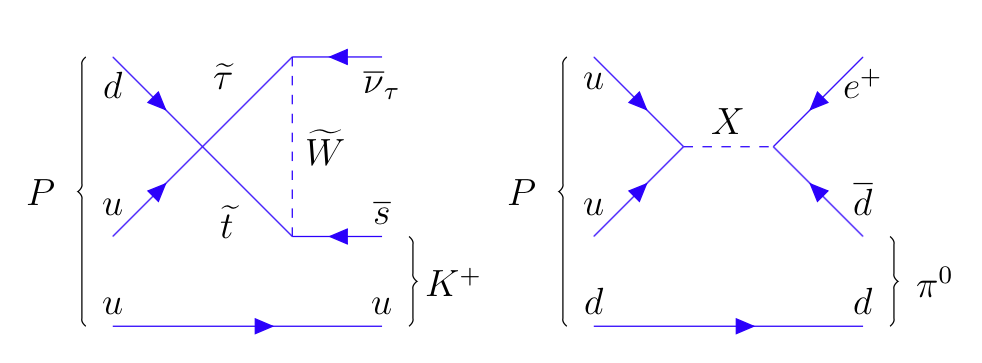
\includegraphics[width=6.5in]{Chapter-1/Images/MandatoryFeynmannDiagrams.png}
\caption{Feynman diagrams for proton decay ``golden modes": $p \rightarrow K^+ \bar{\nu}$ for supersymmetric GUTs on the left and  $p \rightarrow e^+ \pi^0$ for gauge-mediated GUTs  on the right.}
\label{fig:MandatoryFeynmannDiagrams}
\end{figure}


LArIAT tiny active volume makes it impossible for the experiment to place competitive limits on nucleon decay searches.  However,  LArIAT provides excellent data to characterize kaons in liquid argon for the ``LAr golden mode", $p \rightarrow K^+ \bar{\nu}$.  The result of these studies will affect future proton decay searches in LArTPCs.  Previous work has been done to assess the potential identification efficiency for different decay modes in a LArTPC \cite{Bueno2007}, but, as the time of this  writing, no study of kaon selection efficiency in LArTPCs has been performed on data. 
The K$^+$-Ar interaction cross section has never been measured before and can affect the possibility of detecting and measuring kaons when produced in a proton decay event. 
Kaon interactions with argon can distort the kaon energy spectrum as well as change the topology of single kaon events. In a LArTPC, non-interacting kaons appear as straight tracks with a high ionization depositions at the end (Bragg peak). The topology of interacting kaons can be quite different. In case of elastic scattering, a distinct kink will be present in the track. In case of inelastic scattering the Bragg peak will not be present and additional tracks will populate the event.
Performing the total hadronic K$^+$-Ar cross section measurement on data serves the double purpose of identifying the rate of ``unusual" topologies (kinks and additional tracks) and of developing tools for kaon tracking in LAr.

\subsubsection{K$^{+}$Ar Cross section in the Context of Light Mesons Interaction with Nuclei}
\label{sec:theoryStrangeMeson}
The intrinsic value of the total hadronic K$^{+}$-Ar cross section measurement is that kaon interactions complement the measurements of $\pi$ interactions as a probe of  hadron interaction inside the nucleus in the strange sector.  
\textcolor{red}{High theoretical interest in probing constituent quark model of nuclear structure with
KAON-NUCLEON INTERACTIONS CHIEDI REFERENZE A FLAVIO}


%Total cross sections for the interaction of mildly relativistic kaons with several nuclei were derived from transmission experiments performed at the alternating-gradient synchrotron in Brookhaven National Laboratory. The high precision of these cross sections ~about 1\% led to analyses of the data in terms of KN nucleus potentials, based on the expectation that the KN nucleus interaction is simply related to the KN interaction. In particular, in this energy range the KN interaction does not vary strongly with energy and together with the relative weakness of the interaction, one expects that optical potentials close to the ??tr?? approximation ~see below will be capable of describing the data. However, all such analyses showed disagreement between calculation and experiment at the level of 5?15\%, which caused speculations about modifications in the nuclear medium of the KN interaction @5?8#. 

\subsubsection{Signal Signatures}\label{sec:KSignalSignature}
%%%%%%%%%%%%%%%%%%%%%%%%%%%%%%%%%%%%%%%%%%%%%%%%%%%%%%%%%%%%%%%%%%%%%%%%%%%%%%%%%
The interaction of a mildly relativistic charged kaon with an argon nucleus is determined largely by the strong force. The total hadronic K$^{+}$-Ar interaction cross section is defined as the one related to the single (hadronic) process driven only by the strong interaction.
In this case, ``total" indicates all strong interactions regardless of the final state. This condition purposefully includes both elastic and inelastic (reaction) channels. Indeed, the total cross section section can be then decomposed into
$$\sigma_{Tot} = \sigma_{Elastic}+ \sigma_{Reaction}.$$


%For this analysis, kaons are selected from the LArIAT beamline in the momentum range between \textcolor{red}{500} MeV/c and \textcolor{red}{1000} MeV/c (see Fig \ref{fig:TOFK}).

%\begin{figure}[hpbt]
%\centering
%\includegraphics[width=5in]{Chapter-1/Images/KaonTOF}
%\caption{Time of flight versus momentum distributions as produced by the LArIAT TOF and Wire Chambers systems. The Kaon population lies between the proton and the muon/pion populations, allowing PID of Kaons in the beam line.  }
%\label{fig:TOFK}
%\end{figure}

For the LArIAT cross section analysis, the kaons considered span a momentum inside the TPC from 800 MeV/c and 100 MeV/c. In this energy range, the relevant K-Nucleon interactions are according to \cite{fesbach1992theoretical}:

\begin{align}
K^{+} + N &\rightarrow K^{+} + N\textit{ (elastic)}\\
K^{+} + n &\rightarrow K^{0} + p\textit{ (elastic)}\\
K^{+} + N &\rightarrow K + N + \pi \textit{ (inelastic)}\\
K^{+} + N &\rightarrow K^{*} + N\textit{ (inelastic)}.
\end{align}

\subsubsection{Previous Measurements: Lighter and Heavier Nuclei}
In general, measurements on kaon cross sections are  extremely scarce. The measurement of the kaon interaction cross section would bring the additional benefit of reducing the uncertainties associated  with hadron interaction models adopted in MC simulations for argon targets, beneficial for both proton decay studies and kaon production from neutrino interaction studies, where the  uncertainties for final state interaction models are big \cite{Drakoulakos:2004gn}. 

Figure \ref{fig:Friedmann} shows a 1997 measurement on several elements as performed by  Friedmann et al.  \cite{Friedman:1997eq}. As a reference, this paper measures a $\sigma_{Tot}$ for Si of  366.5  $\pm$  4.8 mb and a $\sigma_{Tot}$ for Ca of 494.6  $\pm$ 7.7 mb at 488 MeV/c.  The cross section for argon is expected to lie in between these two measurements. 
Additional data on the kaon cross section are provided by Bugg et al. \cite{PhysRev.168.1466}. Bugg performs a measurement of the total 
K$^+$ and K$^-$ cross sections on protons and deuterons over the range of 0.6-2.65 GeV/c, as well as a measurement of the total K$^+$ and K$^-$  cross sections on carbon for a number of momenta; the results of this paper on carbon are reported in Figure \ref{fig:Bugg}.



\begin{figure}
\captionsetup{justification=raggedright}  
	\begin{minipage}[t]{.53\textwidth}  
	  \centering  
	   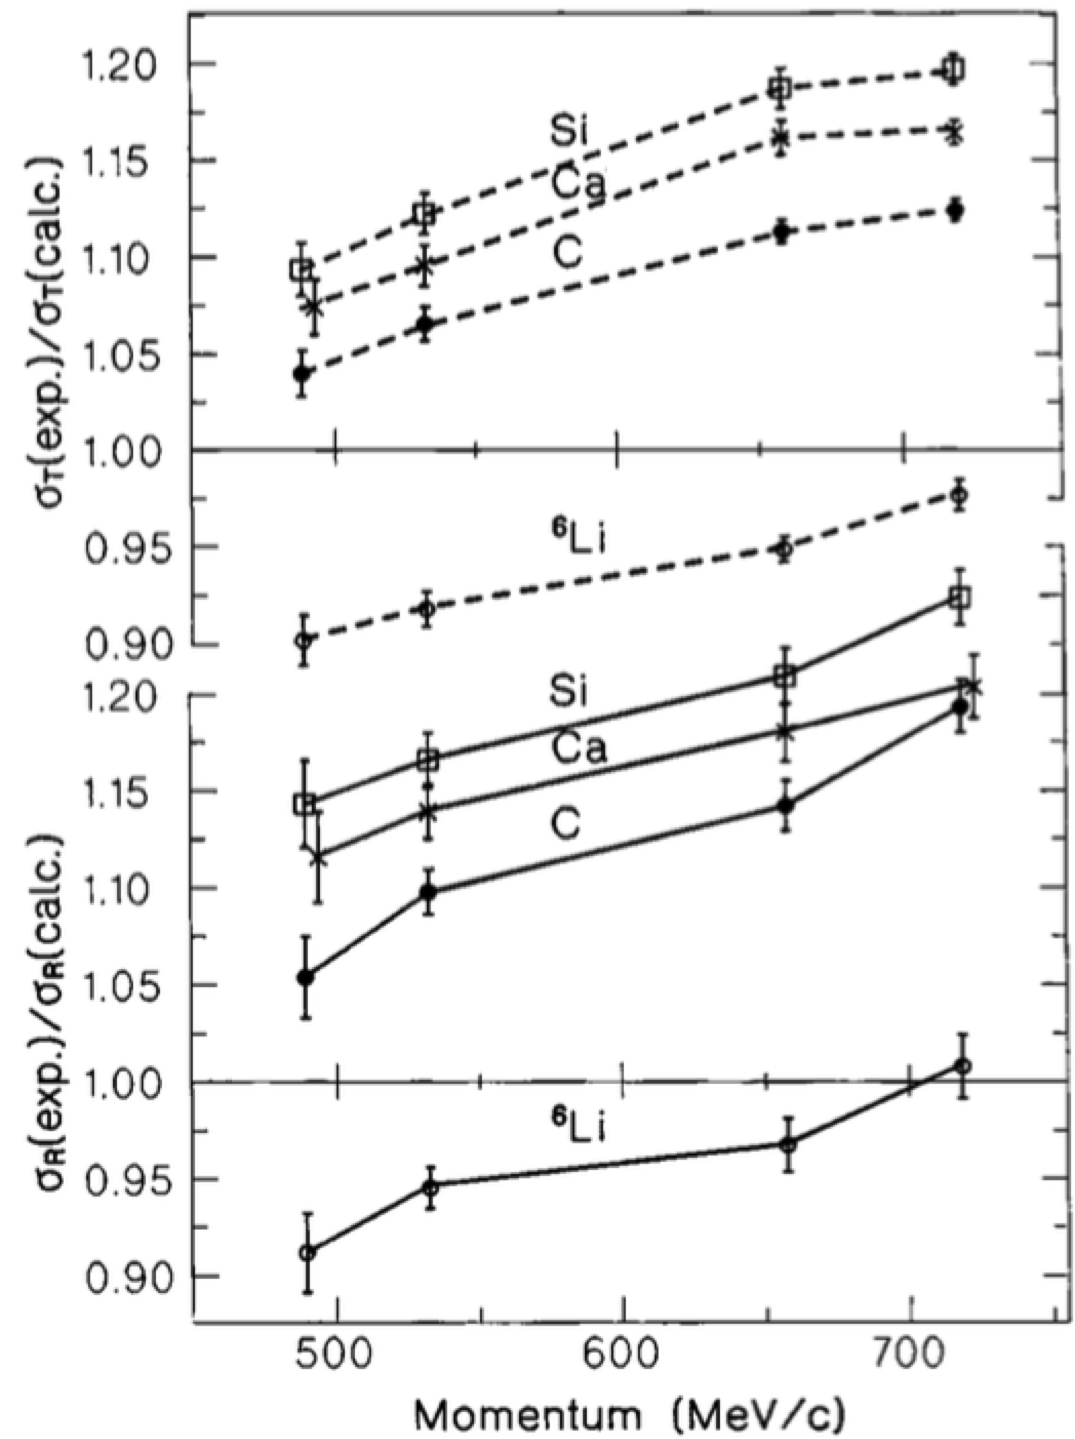
\includegraphics[width=3in]{Chapter-1/Images/Friedmann.png}
	   	        \caption{Ratios between experimental and calculated cross sections as from \cite{Friedman:1997eq}. Top: Total cross sections. \\Bottom: reaction cross sections.}
        \label{fig:Friedmann}
	\end{minipage}%  
	\begin{minipage}[t]{0.53\textwidth}  
	  \centering  
	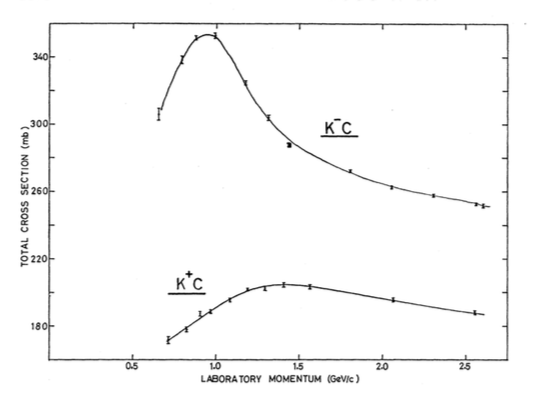
\includegraphics[width=3in]{Chapter-1/Images/Bugg.png}
        \caption{Total K$^+$  and K$^-$ cross sections on carbon as from \cite{PhysRev.168.1466}.}
        \label{fig:Bugg}
	\end{minipage}
	\par
\end{figure}



%%%%%%%%%%%%%%%%%%%%%%%%%%%%%%%%%%%%%%%%%%%%%%%%%%%%%%%
%% PRETTY EVENT DISPLAY WITH TEXT, NOT SURE IF USEFUL
%\begin{figure}[h!]
%\centering
%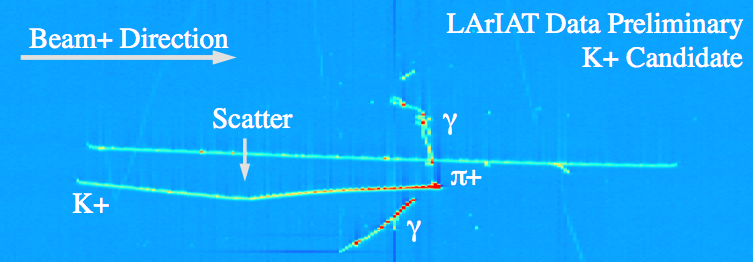
\includegraphics[width=6.5in]{Chapter-1/Images/KLariat.png}
%\caption{LArIAT Data $K^+$ candidate. $K^+$ enters TPC, undergoes a hadronic scatter, and then decays into $\pi^+$ and $\pi^0$. The the $\pi^0$ decays into 2 photons while the $\pi^+$ stops quickly in the TPC. Collection plane view.}
%\label{Fig:KLariat}
%\end{figure}

%Fig \ref{Fig:KLariat} shows a $K^+$ candidate event in the LArIAT TPC. Following the kaon candidate track from left to right, two important elements are visible by eye: a change in the K momentum due to hadronic scatter and a Bragg peak by the end of the track due to an augment of ionization as the kaon slows down in the TPC. The track "kink" is only visible thanks to the millimetric spacial resolution of the TPC, while the Bragg shows the calorimetric power of this technology. The kaon in this event decays hadronically into $\pi^+$ and $\pi^0$. The the $\pi^0$ decays into 2 photons while the $\pi^+$ stops quickly in the TPC. The ability to distinguish the topology of this decay from the most frequent one, i.e. $K^+\rightarrow\mu^+\nu$, remarks the versatility of the LArTPC technology.
%%%%%%%%%%%%%%%%%%%%%%%%%%%%%%%%%%%%%%%%%%%%%%%%%%%%%%%




 \subsubsection{Kaon Interaction Cross Section for thin target in Geant4}
Since the kaon cross section in argon has never been measured before, simulation packages tune kaon transportation in argon by extrapolation from lighter and heavier nuclei. LArIAT uses the Geant4 suite for particle transportation.  Since kaon data on carbon are available, we used it as a metric to evaluate the Geant4 prediction performances.  Figure \ref{fig:TrueCarbon} shows the total hadronic cross section for carbon implemented in Geant4 10.01.p3 overlaid with the Bugg and Friedman data. Unfortunately, the current version of Geant4 does not reproduce the data for carbon closely. On one hand, this evidence makes us even more wary when using the Monte Carlo in simulating the kaon-argon interactions. On the other, it further highlights the importance of the kaon measurement.



\begin{figure}
\captionsetup{justification=raggedright}  
  \centering  
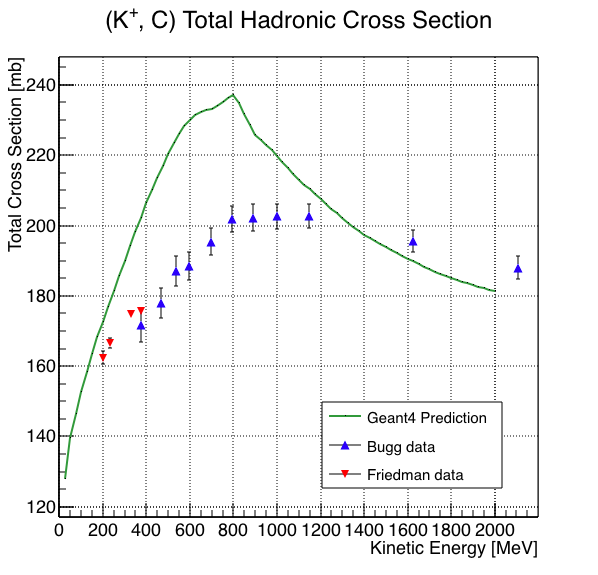
\includegraphics[width=3in]{Chapter-1/Images/CarbonG4.png}
\caption{total hadronic cross section for carbon implemented in Geant4  10.01.p3  with overlaid with the Bugg and Frideman data.}
\label{fig:TrueCarbon}
\end{figure}







\chapter{Liquid Argon Detectors at the Intensity Frontier}\label{ch:2}
{\raggedleft ``\emph{Don't you know, honey,} \par}
{\raggedleft \emph{Ain't nobody ever gonna love you, the way I try to do?}"\par}
{\raggedleft -- Janis Joplin, Cry Baby, 1971 -- \par}
\vspace{0.5cm}

In the next few years, LArTPCs will  be the tools to answer some of the burning questions in neutrino physics today.  This chapter illustrates the operational principles of this detector technology, as well as the scope of the key detectors in the US liquid argon program -- SBN, DUNE and LArIAT.


\section{The Liquid Argon Time Projection Chamber Technology}
In this section, we outline an extremely brief history of Time Projection Chambers as particle detectors, focusing on their incarnation as Argon detectors for neutrino physics. We further describe the working principles of Liquid Argon Time Projection Chambers, leading  to the description of the event reconstruction in LArTPC.

\subsection{TPCs, Neutrinos \& Argon}
David Nygren designed the first Time Projection Chamber (TPC) in the late 1970s~\cite{FirstTPC} for the  PEP-4 experiment, a detector  apt to study electron-positron collisions at the PEP storage ring at the SLAC National Accelerator Laboratory.
From the original design  in the seventies -- a cylindrical chamber filled with methane gas -- the TPC detector concept has seen many incarnations, the employment of several different active media and a variety of different particle physics applications, including, but not limited to the study of electron/positron storage rings (e.g. PEP4, TOPAZ, ALEPH and DELPHI), heavy ions collisions in fixed target and collider experiments (e.g. EOS/HISS and ALICE ), dark matter (ArDM), rare decays and capture (e.g. TRIUMP, MuCap),  neutrino detectors and nucleon decay (ICARUS, SBN, DUNE), and neutrino less double beta decay (Next). A nice review of the history of TPCs and working principles is provided in \cite{0034-4885-73-11-116201}.

Several features of the TPC technology make these detectors a more versatile tool compared to other ionization detectors and explain such a wide popularity. TPCs are the only electronically read detector which deliver simultaneous  three-dimensional track information and a measurement of the particle energy loss. Leveraging on both tracking and calorimetry,  particle identification (PID) capabilities are enhanced  over a wide momentum range. 

Historically, the active medium in ionization detectors has been in the gaseous form. Carlo Rubbia first proposed the use of a Liquid Argon TPC for a neutrino experiment, ICARUS \cite{Rubbia:1977zz}, in 1977.  Using nobles elements in the liquid form for neutrino detectors is advantageous for several reasons.  The density of liquids is $\sim$1000 times greater than gases, augmenting the number of targets for neutrino's interaction in the same volume, in a effort to balance the smallness of neutrino cross section. Since the energy loss of charged particle is proportional to the target material density, as shown in the Bethe-Block equation (eq. \ref{eq:BB}), the increased density reflects into a proportionally higher energy loss, enhancing the calorimetry capability of detectors with a liquid active medium. Additionally, the ionization energy of liquids is smaller than gasses by the order of tens of eV. Thus, at the passage of charged particles, liquids generally produce more ionization electrons than gases for the same deposited energy, forcing the particles to deposit more energy in a shorter range. The downside of using noble liquid elements in experiments is that they require expensive cryogenic systems to cool the gas until it transitions to its the liquid form.
The properties of liquid argon in comparison liquid xenon -- a popular choice for dark matter and neutrinoless double beta decay detectors -- are summarized in table \ref{tab:properties}.  Albeit xenon would be more desirable than argon given some superior properties such as lower ionization energy and higher density and light yield, argon relative abundance abates the cost of argon compared to xenon, making argon a more viable choice for the construction of ton  (and kilo-ton) scale neutrino detectors. 




\begin{table}[]
\centering
\begin{tabular}{|l|c|c|}\hline
Element & LAr & LXe \\
\hline
\hline
Atomic Number &  18 &54 \\
Atomic weight A & 40  & 131\\
Boiling Point Tb at 1 atm & 87.3 K & 165.0 K\\
Density  & 1.4 g/cm$^3$& 3.0 g/cm$^3$\\
Radiation length  & 14.0 cm& 2.8 cm \\
Moliere Radius  &10.0 cm& 5.7 cm\\
Work function  & 23.6 eV&15.6 eV\\
Electron Mobility at $E_{field} =10^4$ V/m &0.047 m$^2$/Vs& 0.22 m$^2$/Vs\\
Average dE/dx MIP  & 2.1 MeV/cm&3.8 MeV/cm\\
Average Scintillation Light Yield & 40000 $\gamma$/MeV&42000 $\gamma$/MeV\\
Scintillation $\lambda$  &128 nm&175 nm\\
\hline
\end{tabular}
\caption{LAr, LXe summary of properties relevant for neutrino detectors.}
\label{tab:properties}
\end{table}


LArTPCs are some times referred as to ``electronic" bubble-chambers, for the similarity in the tracking and energy resolution which is coupled with an electronic readout of the imaging information in LArTPCs. Compared to these historic detectors however, LArTPC bestow tridimensional tracking and a self triggering mechanism provided by the scintillation light in the liquid argon.  An event display of a $\nu_\mu$ CC interaction candidate in the MicroBooNE detector is shown in picture \ref{fig:NuEvd} to display the level of spatial details these detectors are capable of; the color scale of the image is proportional to the energy deposited, hinting to these calorimetry capabilities of the detectors.
\begin{figure}[hbpt]
\centering
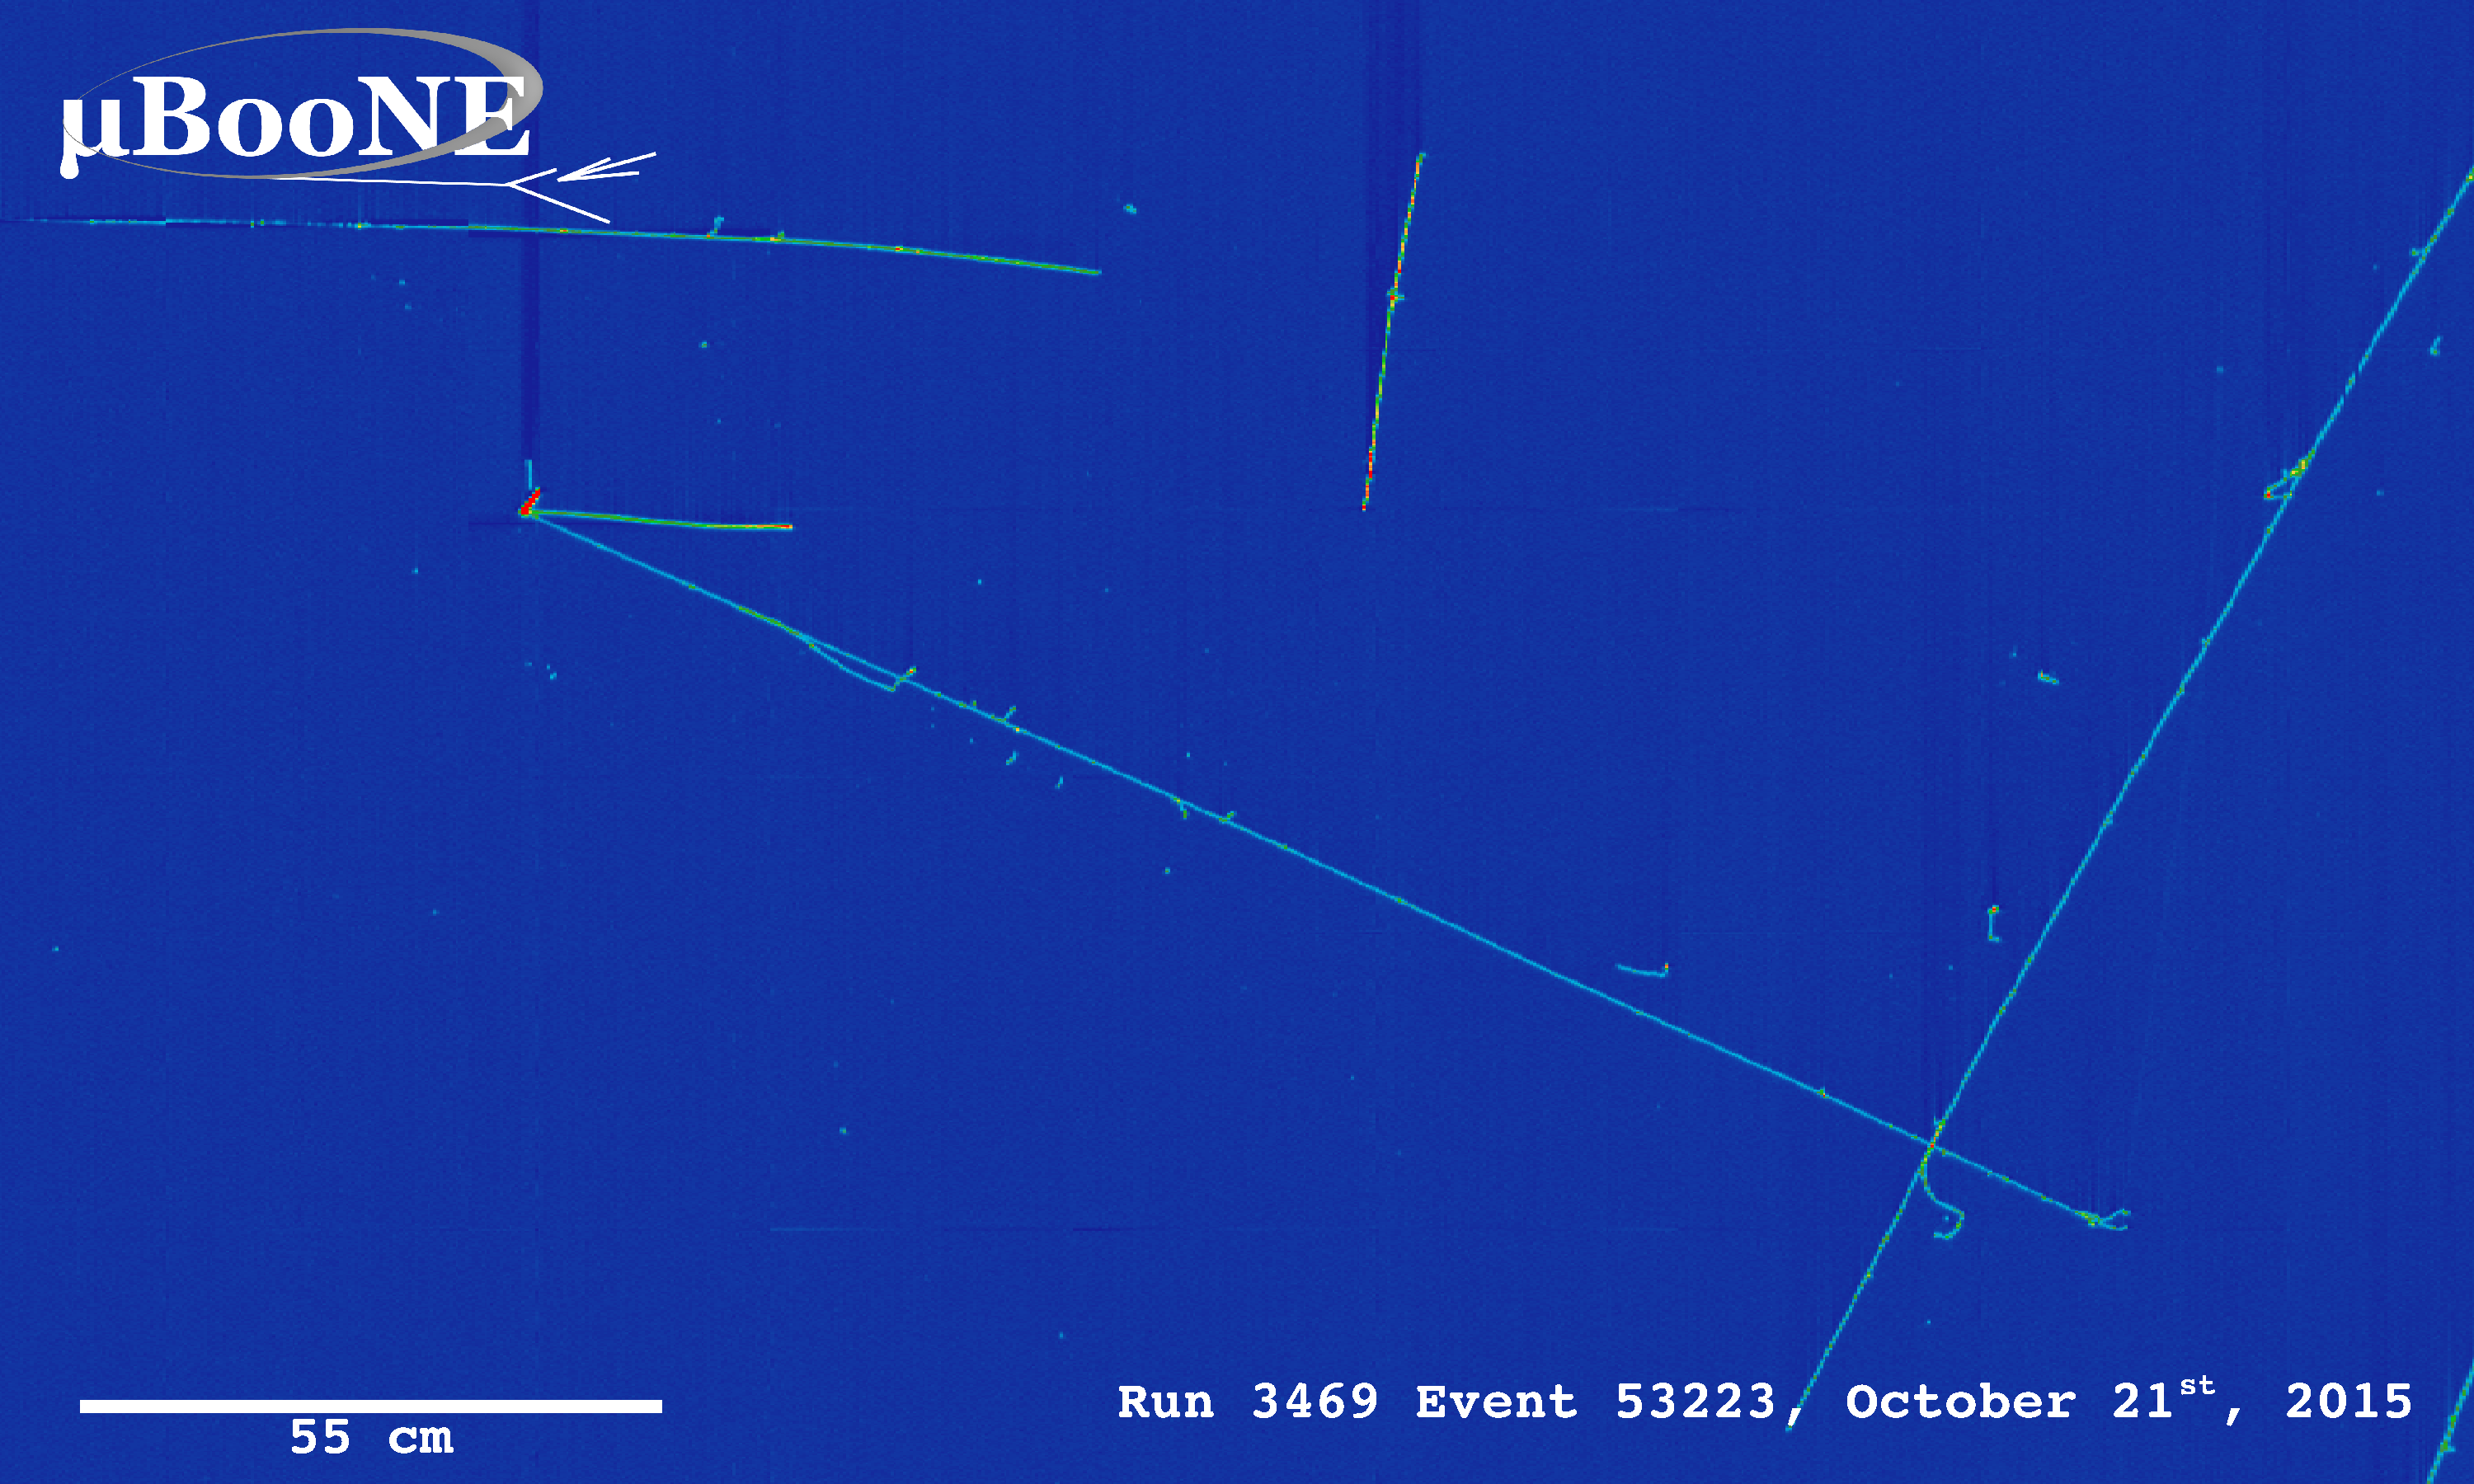
\includegraphics[width=\textwidth]{Chapter-2/Images/run3469_subrun1064_event53223_col.pdf}
\caption{Event display of a $\nu_\mu$ CC interaction candidate in the MicroBooNE detector.}
\label{fig:NuEvd}
\end{figure}



\subsection{LArTPC: Principles of Operation}\label{sec:LArTPCWorkingPrinciple}

\begin{figure}[hbpt]
\centering
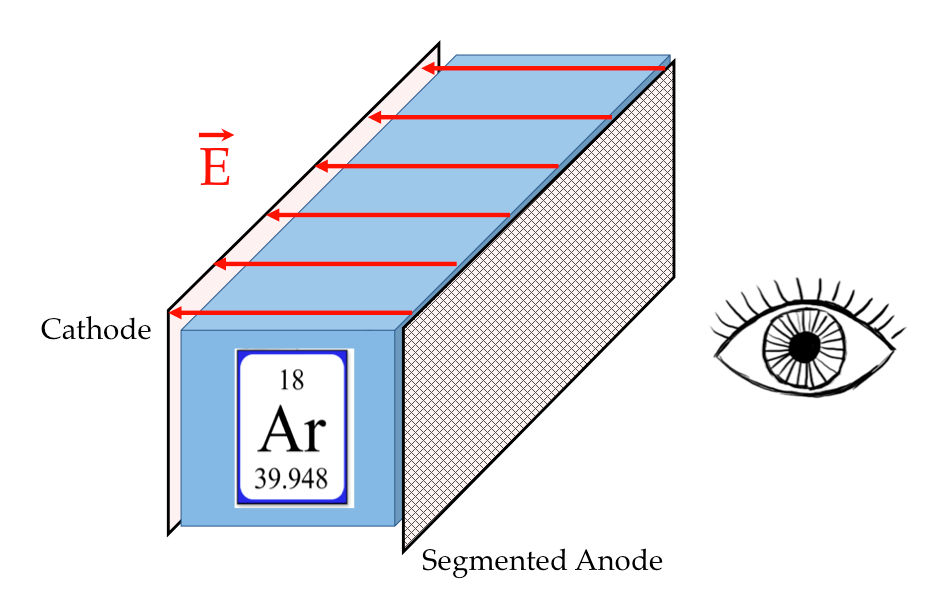
\includegraphics[width=\textwidth]{Chapter-2/Images/Cartoon.png}
\caption{A cartoonish sketch of a LArTPC.}
\label{fig:cartoon}
\end{figure}


To the bare bones, a LArTPC is a bulk of liquid argon sandwiched in a flat capacitor, equipped with a light collection system, as the cartoon in \ref{fig:cartoon} shows. A uniform electric field of the order of 500 V/cm is maintained constant between the faces of the capacitor. The anode is sensitive to ionization charge and it is usually made of two or more planes segmented into several hundreds parallel sense wires a few millimeters apart; different geometries for the anode segmentation are under study \cite{1748-0221-8-07-P07002}. 

Argon ionization and scintillation are the processes leveraged to detect particles in the LArTPC active volume.  When a ionizing radiation traverses the argon active volume it leaves a trail of ionization electrons along its trajectory and it excites the argon producing scintillation light -- details on the production and detection of ionization charge and scintillation light are provided in \ref{sec:light} and \ref{sec:light} respectively. The optical detector sees the argon scintillation light in matters of nanoseconds. This flash of light determines the start time of an event in the chamber, $t_0$. The uniform electric field drifts the ionization  electrons from the production point towards the anode in order of hundreds of microseconds or more depending on the chamber dimensions\footnote{The ionized argon also drifts, but  in the opposite directions compared to the electrons. Since the drift time is proportional to the particle mass,  the ions' drift time is much longer than the electrons'.  Ionized argon is collected on the cathode which is not instrumented, so it is not used to infer information about the interactions in the chamber.}. The anode sense wires see either an induced current by the drifting ionization charge (on induction planes) or an injection of such charge (collection plane).    An appropriate choice of the voltage bias on each wire plane assures ideal charge transparency, so that all the ionization charge is collected on the collection plane and none on the induction planes.  

The arrival time of the charge on the anode sense wires is used to measure the position of the original ionizing radiation in the drift direction. In fact, since the constant electric field implies that the drift velocity is also constant, the position of the original ionization is simply given by the multiplication of the drift velocity by the drift time, where the ``drift time" is the difference between $t_0$ and the charge arrival time on the wire planes. The spacial resolution on this dimension is limited by the time resolution of the electronics or by longitudinal diffusion of the electrons.
The spatial information on the different wire planes maps a bi-dimensional projection of the interaction pattern in the plane perpendicular to the drift direction. The spacial resolution on this dimension is limited by the transverse electron diffusion in argon and by the grain of the anode segmentation, i.e. the spacing between the wires in the sense planes \cite{DERENZO1974319}.  The off-line combination of the 2-D information on the wire planes with the timing information allows for the 3D reconstruction of the event in the chamber.

Since the charge deposited by the ionizing radiation is proportional to the deposited energy and the charge collected on the sense plane is a function of the deposited charge, LArTPCs allow the measurement of the energy deposit in the active volume. Effects due to the presence of free charge and impurities in the active volume, such as a finite electron lifetime, recombination and space charge, complicate the relationship between deposited and collected charge affecting the measurement of the particle's energy, as described in the next section.
 
\subsection{Liquid Argon: Ionization Charge}\label{sec:charge}
The mean rate of energy loss by moderately relativistic elementary charge particles heavier than electrons is well described by the modified Bethe-Bloch \cite{Patrignani:2016xqp} equation
\begin{eqnarray}
			- \frac{dE}{dx} = K z^2 \frac{Z}{A} \varrho \frac{1}{\beta^2} \left[ \frac{1}{2} \ln{\frac{2 m_e c^2 \beta^2 \gamma^2 T_{max}}{I^2}} - \beta^2 - \frac{\delta}{2}\right] ,
			\label{eq:BB}
\end{eqnarray}
where  $z$ is the number of unit charge of the ionizing radiation, $Z$, $A$  and $\varrho$ are the atomic number, mass number and density of the medium,  $m_e$  is the electron mass, $\gamma = \frac{\beta}{\sqrt{1-\beta^2}} $ is the Lorentz factor of the ionizing radiation,  $T_{max}$ is the maximum kinetic energy which can be
imparted to a free electron in a single collision, $I$ is the mean excitation energy on eV,  $\delta$ is the  density correction and $K = 0.307 075 \text{ MeV g}^{-1}\text{ cm}^2$ is a numerical conversion factor. The Bethe-Bloch treats the energy loss by an ionizing radiation via quantum-mechanical collisions producing ionization or an excitation in the medium as an uniform and continuous process. The density correction  terms becomes relevant for incident particle with high energy, where screening effects due to the polarization of the medium by high energy particles occur.

Excitation and ionization of the detector medium occur in similar amounts. Since the ionizing collisions occur randomly, we can parametrize their number $k$ in a segment of length $s$ along the track  with a Poissonian function
\begin{equation}
P(k) = \frac{s^k}{k! \lambda^k} e^{-s/ \lambda }, 
\end{equation}
where $\lambda = 1/N_{e}\sigma_i$, with $N_{e}$ being the electron density of $\sigma_i$ the ionization cross-section per electron.  About 66\% of the ionizing collisions in Argon produce only a single electron/ion pair \cite{0034-4885-73-11-116201}; in the other cases, the transferred kinetic energy is enough for the primary electron to liberate one or more secondary electrons, which usually stay close to the original pair.  
Occasionally, electrons can receive enough energy to be ejected with high energy, forming a so-called ``$\delta$-ray": a detectable  short track off the particle trajectory, as shown in figure \ref{fig:delta}. 
The average number of $\delta$-ray  with energy E$>$E$_0$ per cm follows the empirical form
\begin{equation}
P(E>E_0) \sim \frac{y}{\beta^2 E_0},
\end{equation}
where $y$ is an empirical factor depending on the medium (0.114 for  gaseous Ar), and $\beta$ is $v/c$.

\begin{figure}[hbpt]
\centering
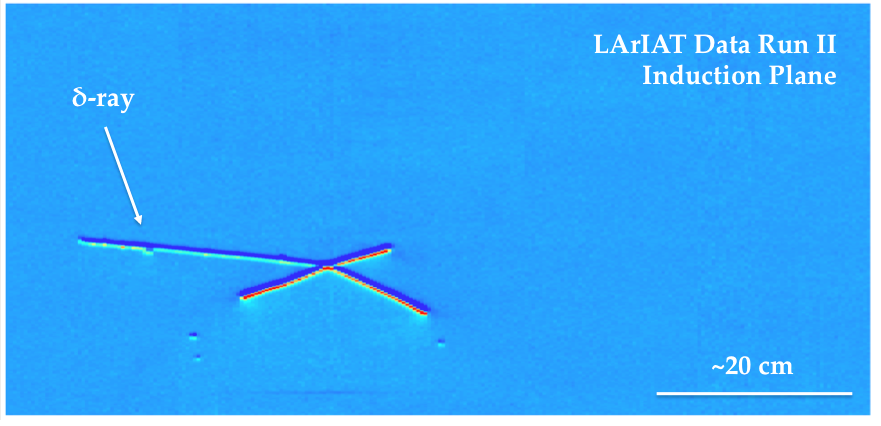
\includegraphics[width=\textwidth]{Chapter-2/Images/Delta.png}
\caption{Events display for a LArIAT pion absorption candidate on the induction plane, with highlighted delta ray.}
\label{fig:delta}
\end{figure}


		
\subsubsection{Purity \& Electron Life Time }
The presence of electronegative contaminants in liquid argon, such as oxygen $O_2$ and water $H_2O$, is particularly
pernicious, since these molecules quench the charge produced by the ionizing radiation.  Thus, amount of charge per unit of length $dQ/dx$ collected on the collection plane depends on the charge's production point in the detector: ionization produced  close to the cathode will see more impurities along its journey to the collection plane than ionization produced close to the anode, resulting in greater attenuation of its charge. As a result,  the amount of charge collected on the sense wires as a function of the traveled distance follows an exponential decay trend. The traveled distance is generally measured in terms of drift time and the  characteristic time constant of the exponential decay is called electron lifetime $\tau_e$. Figure \ref{fig:Elifetime} shows the typical life time for LArIAT data. The procedure to measure the electron lifetime in LArIAT is outlined in \cite{LArIATLifeTime}. LArIAT small drift distance (47 cm) allows for a relatively short electron life time. The life time for bigger detectors such as MicroBooNE, whose drift distance is 2.6 m, needs to be of the order of tens of milliseconds to allow a charge collection usable for physics analyses. Energy reconstruction in LArTPC applies a correction for the finite lifetime to calibrate the detector calorimetric response; details for LArIAT are provided in Section \ref{ch:energyCalibration}.

\begin{figure}[hbpt]
\centering
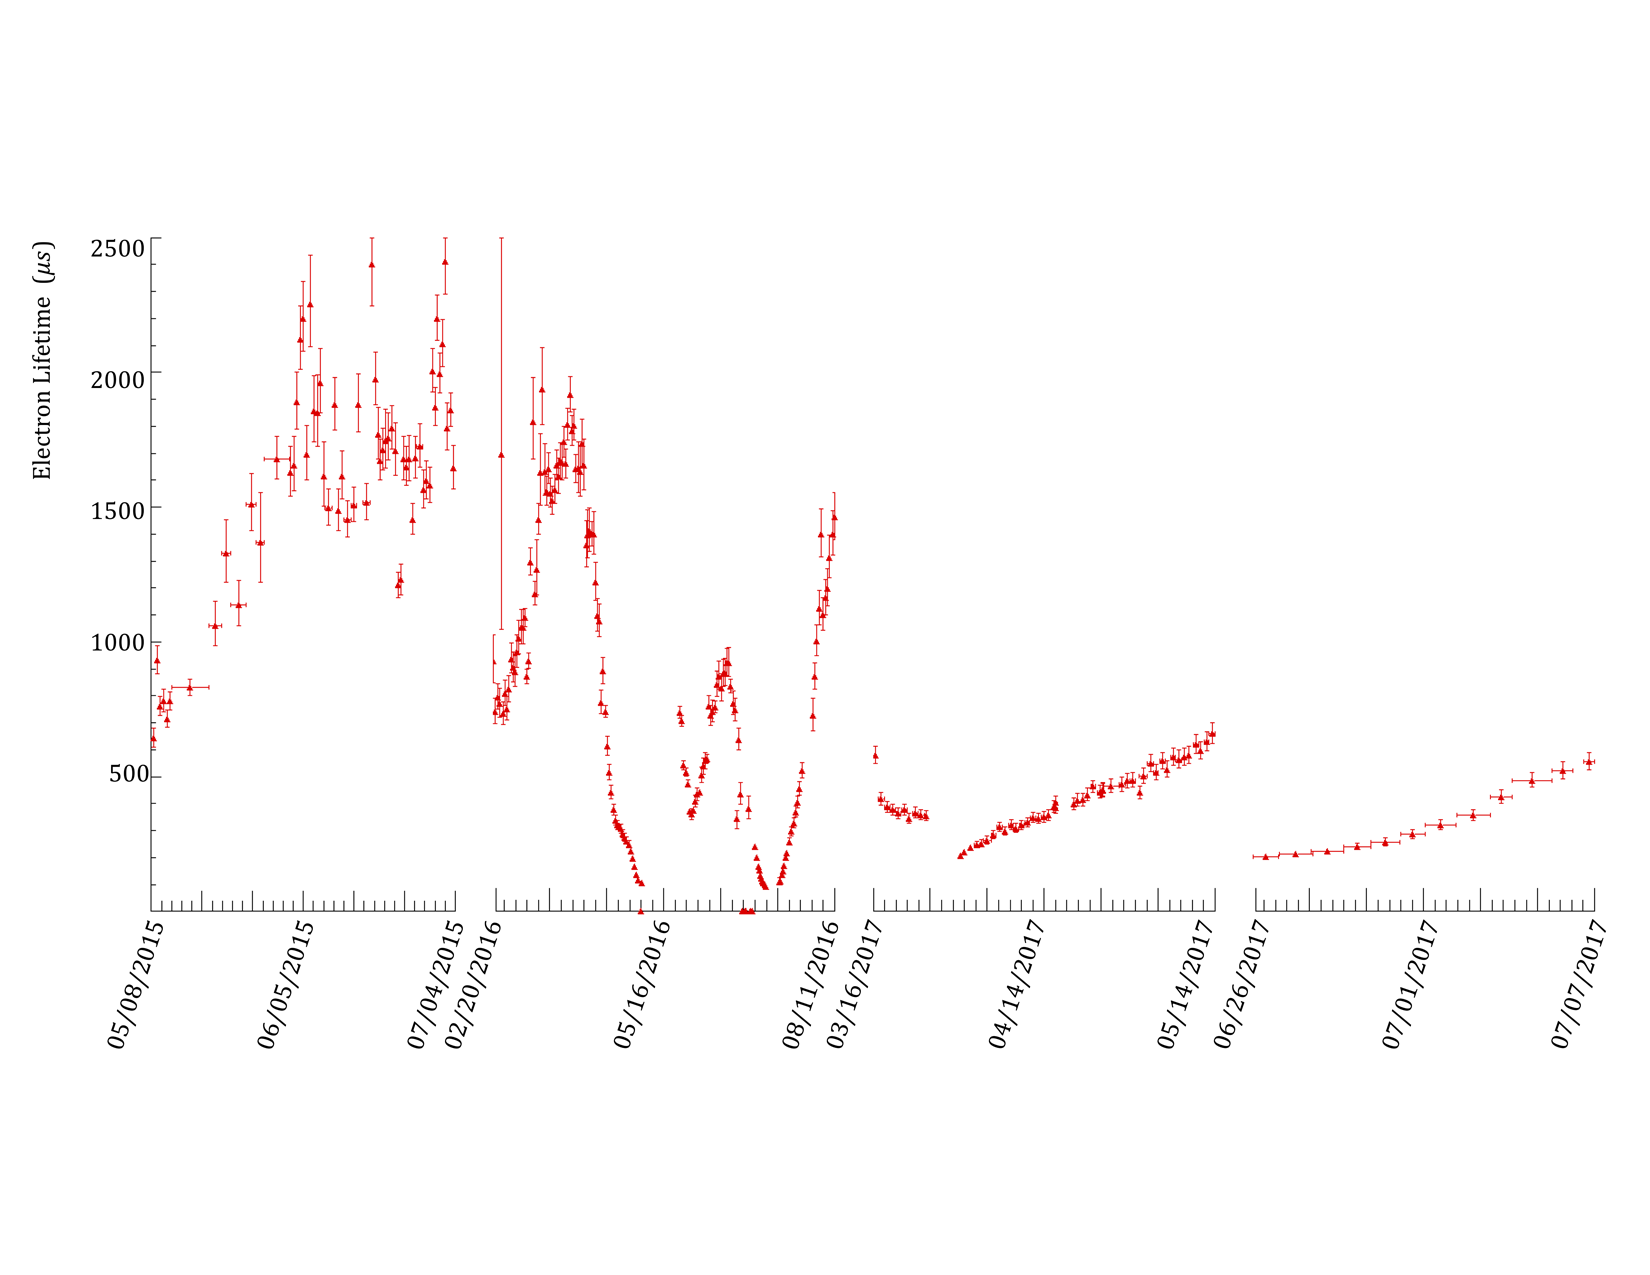
\includegraphics[width=\textwidth]{Chapter-2/Images/ELifetime.png}
\caption{Electron lifetime during the LArIAT run period \cite{detectorPaper}.}
\label{fig:Elifetime}
\end{figure}


LArTPCs use  hermetically sealed and leak-checked vessels to abate the leakage and diffusion of contaminants into the system. The liquid argon filling of the volume occurs after the vessel is evacuated or purged with gaseous argon \cite{1748-0221-9-07-P07005} to reduce remaining gases in the volume. Even so, the construction of a pure tank of argon is unviable, as several sources of impurity remain.  In particular, impurities can come from the raw argon supply, the argon filtration system and from the outgassing from internal surfaces. Outgassing is a continuous diffusive process  producing contaminants, especially water, even after the vessel is sealed, particularly from materials in the ullage region\footnote{While the liquid argon low temperature reduces outgassing in the liquid, this process remains significant for absorptive material (such as plastic) above the surface of the liquid phase.}.  Since research-grade argon comes from the industrial distillation of air, the impurities with the highest concentration are nitrogen, oxygen and water, generally maintained under the 1 part per million level by the vendor.  Even so, a higher level of purity is necessary to achieve a free electron life time usable in meter scale detectors. Thus, argon  is constantly  filtered in the cryogenic system, which reduce the oxygen and water contamination to less than 100 parts per trillion. The filtration system depends on the size and drift distance of the experiment and, for experiments on several meters scale, it includes an argon recirculation system.

%% Life time value for LArIAT


\subsubsection{Recombination Effect}
After production, ionization electrons thermalize with the surrounding medium and may recombine with nearby ions. Recombination might occur either between the electron and the parent ion through Coulomb attraction, as described in the geminate theory  \cite{PhysRev.54.554}, or thanks to the collective charge density of electrons and ions from multiple ionizations in a cylindrical volume surrounding the particle trajectory, as described in the  columnar model \cite{Jaff1913}. 
Consideration on the  average electron-ion distance and the average ion-ion distance for argon show that the probability of geminate recombination is low; thus recombination in argon is mainly due to collective effects\cite{1748-0221-8-08-P08005}.  Since protons, kaons and stopping particles present a higher ionization compared to MIPs, recombination effects are more prominent when considering the reconstruction of energy deposited by these particles.

Theoretical descriptions of recombination based on the Birks model and the Box model are provided in \cite{0370-1298-64-10-303} and  \cite{PhysRevA.36.614}, respectively. The Birks model assumes a gaussian spatial distribution around the particle trajectory during the entire recombination phase and identical charge mobility for ions and electrons. The Box model also assumes that electron diffusion and ion mobility are negligible in liquid argon during recombination.
In these models, the fraction of ionization electrons surviving recombination is a function of the number of ion-electron pairs per unit length, the electric field, the average ion-electron separation distance after thermalization and the angle of the particle with respect to the direction of the electric field -- plus the diffusion coefficient in the Birks model. Given the stringent assumptions, it is perhaps  not surprising that these models are in accordance to data only in specific regimes: the Birks model is generally used to describe recombination for low dE/dx, the Box model for high dE/dX.
In LArTPC, the ICARUS and ArgoNeut experiments have measured recombination in \cite{Amoruso:2004dy} and \cite{1748-0221-8-08-P08005} respectively. Since LArIAT uses the refurbished ArgoNeut TPC and cryostat at the same electric field,  LArIAT currently corrects for recombination using the ArgoNeut measured recombination parameters in \cite{1748-0221-8-08-P08005}.


\subsubsection{Space Charge Effect}
Slow-moving positive argon ions created during ionization can build-up in LArTPC, causing the distortion of the
electric field within the detector. This effect, called  ``space charge effect" leads to a displacement in the reconstructed position of the signal ionization electrons. In surface LArTPCs the space charge effect is primarily due to the rate of ionization produced by cosmic rays which is slowly drifting in the chamber at all times. Surface LArTPC of the size of several meters are expected to be modestly impacted from the space charge effect, where charge build-up create anisotropy of the electric field magnitude of the order of  5\% at a drift field of 500 V/cm \cite{SpaceCharge}. The smallness of the LArIAT drift volume and its relatively high electric field are such that the effect of  space charge is expected to be negligible. 

%%%%%%%%%%%%%%%%%%%%%%%%%%%%%%%%%%%%%%%%%%%%%%%%%%%%%%%%%%%%%%%
%%%%%%%%%%%%%%%%%%%%%                     Light Detection             %%%%%%%%%%%%%%%%%%%%%%%%
%%%%%%%%%%%%%%%%%%%%%%%%%%%%%%%%%%%%%%%%%%%%%%%%%%%%%%%%%%%%%%%
\subsection{Liquid Argon: Scintillation Light }\label{sec:light}
Liquid argon emits scintillation light at the passage of charged particles. LArTPCs  leverage this property to determine when the ionization charge begins to drift towards the anode plane. %Scintillation light can also be used for particle identification, as discussed in the next sections.

\subsubsection{Scintillation Process}
Scintillation light in argon peaks in the ultraviolet at a 128 nm, shown in comparison to Xenon and Kypton in Figure  \ref{fig:ArLight}, from \cite{Morikawa1989}. The light yield collected by the optical detector depends on the argon purity, the electric field, the dE/dx and particle type, averaging at the tens of thousands of photons per MeV. 

\begin{figure}[hbpt]
\centering
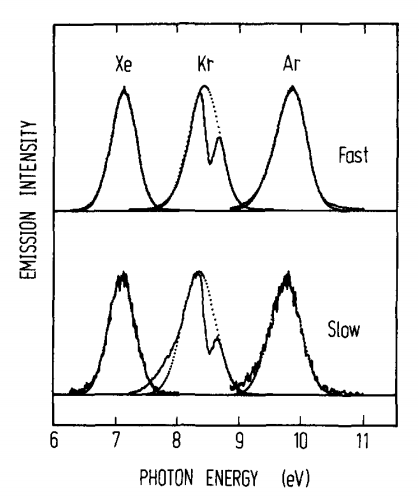
\includegraphics[scale=0.5]{Chapter-2/Images/Light.png}
\caption{Emission spectra of the fast and slow emission components in Xenon, Kypton and Argon according to \cite{Morikawa1989}. The dotted lines correspond to the Gaussian fits. }
\label{fig:ArLight}
\end{figure}




The de-excitation of Rydberg dimers in the argon is responsible for the scintillation light. 
Rydberg dimers exist in two states:  singlets and a triplets. The time constant for the singlet radiative decay is 6 ns, resulting in a prompt component for the scintillation light. The decay of the triplet is delayed by intersystem crossing, producing a slow component with a time constant of $\sim$~1500 ns.  ``Self-trapped exciton luminescence" and  ``recombination luminescence" are the two processes responsible for the creation of the Rydberg dimers \cite{Jones:2015bya}. In the first process, a charged particle excites an argon atom which becomes self-trapped in the surrounding bulk of argon,  forming a dimer; the dimer is in the singlet state 65\% of the times and in the triplet state 35\% of the times. In case of recombination luminescence, the charged particle transfers enough energy to ionize the argon. The argon ion forms a charged argon dimer state, which quickly recombines with the thermalized free electron cloud. Excimer states are produced in the recombination, roughly half in the singlet and half in the triplet state. The light yield dependency on the electric field, on the dE/dx and particle type derives from the role of free charge in the recombination luminescence process. The spacial separation between the argon ions and the free electron cloud depends on the electric field. On one hand, a strong electric field diminishes the recombination probability, leading to a smaller light yield; on the other, it increases the free charge drifting towards the anode plane. Hence, the amount of  measurable charge and light anti-correlates as a function of the electric field.  Ionizing particles in the argon modify the local density of both free electrons and ions depending on their dE/dx. Since the recombination rate is proportional to the square of the local ionization density, highly ionizing particles boost recombination and the subsequent light yield compared to MIPs.  The possibility to leverage this dependency for pulseshape-based particle identification has been shown in \cite{Boulay:2004dk, PhysRevC.78.035801}.

\subsubsection{Effects Modifying the  Light Yield}
The production mechanism through emission from bound excimer states implies that argon is  transparent to its own scintillation light. In fact, the photons emitted from these metastable states are not energetic enough to re-excite the argon bulk, greatly suppressing absorption mechanisms. In a LArTPC however, several processes modify the light yield in between the location where light is produced and the optical detector. In a hypothetical pure tank of argon, Rayleigh scattering would be the most important processes modifying the light yield. Rayleigh scattering changes the path of light propagation in argon, prolonging the time between light production and detection.  The scattering length has been measured to be 66 cm \cite{Ishida1997} , shorter than the theoretical prediction of $\sim$~90 cm \cite{Teague1968}; this value is short enough to be relevant for the current size of LArTPCs detectors. In fact, Rayleigh scattering worsen the resolution on $t_0$, the start time for charge drifting, and  alters the light directionality, complicating the matching between light and charge coming from the same object in case of multiple charged particles in the detector. 

Traces of impurities in argon such as oxygen, water and nitrogen  also affect the light yield, mainly  via absorption and quenching mechanisms. 
Absorption occurs as the interaction of a 128 nm photon directly with the impurity dissolved in the liquid argon.  Differently, quenching occurs as the interaction of an argon excimer and an impurity, where the excimer transfers its excitation to the impurity and  dissociates non-radiatively.  Given this mechanism, it is evident how quenching is both a function of the impurity concentrations and the excimer lifetime.  Since the triplet states live much longer than the singlet states,  quenching occurs mainly on triplet states, affecting primarily the slow component of the light,  reducing the scintillation yield and a shortening of the scintillation time constants.  

The stringent constraints for the electron life time limit the presence of oxygen and water to such a low level that both absorption and quenching on these impurity is not expected to be significant.   Contrarily, the nitrogen level is not bound by the electron life time constraints -- nitrogen being an inert gas, expensive to filter. Thus, nitrogen is often present at the level provided by the vendor. The effects of nitrogen on argon scintillation light have been studied in the WArP R\&D program and at several test stands.
The quenching process induced by nitrogen in liquid Ar has been measured to be proportional to the nitrogen concentration, with a rate constant of $\sim  0.11$ $\mu s^{-1}$ ppm$^{-1}$; appreciable decreasing in lifetime and relative amplitude of the slow component have been shown for contamination as high as a few ppm of nitrogen \cite{1748-0221-5-06-P06003}.
For a nitrogen  concentration of 2 parts per million,  typical of the current generation of LArTPC, the attenuation length due to nitrogen has been measured to be $\sim$30 meters \cite{1748-0221-8-07-P07011}. 



\subsubsection{Wavelength Shifting of LAr Scintillation Light}
Liquid argon scintillation light is invisible for most optical detectors deployed in a LArTPC, such as cryogenic PMTs and SiPMs, since a wavelength of 128 nm is  generally too short to be absorbed from most in glasses, polymers and semiconductor materials. Research on prototype SiPMs absorbing directly VUV light and their deployment in noble gasses experiment is ongoing but not mature \cite{1748-0221-8-01-C01003}. Thus, experiments need to shift the wavelength of scintillation light to be able to detect it.  Albeit deployed in different ways, neutrinos and dark matter experiments commonly use  1,1,4,4-tetraphenyl-butadiene (TPB) to shift the scintillation light. 
TPB  absorbs the vacuum ultraviolet (VUV) light and emits in the visible at $\sim$~425 nm \cite{Burton1973}, with a ratio of visible photon emitted per VUV photon absorbed of $\sim$1.2:1 \cite{GEHMAN2011116}.

Neutrino experiments typically coat their optical detector system evaporating a layer of TPB either directly on the PMTs glass surface or on acrylic plates mounted in front of the PMTs \cite{Acciarri2017}; this technique allows the fast detection light coming directly from the neutrino interaction. Dark matter experiments typically evaporate TPB on reflective foils mounted on the inside walls of the sensitive volume and detect the light after it has been reflected; this technique leads to a higher and more uniform light yield, though scattering effects for both the visible and VUV light augment the propagation time and hinder directionality information\cite{Aalseth2018}. In order to take advantage of both these techniques, hybrid systems with PMT coating and foils are being considered for the next generation of large neutrino detectors. 

\subsection{Signal Processing and Event Reconstruction}\label{sec:SignalProc}
In this section we illustrate the processing and reconstruction chain of the TPC signals, from the pulses on the sense wire to the construction of three dimensional objects with associated calorimetry. Different experiments can chose different software packages for their off line signal processing and event reconstruction, but  a popular choice for  US based  LArTPCs is LArSoft \cite{EricFChurck}. Based on the Art framework \cite{Green:2012gv}, LArSoft is an event-based toolkit to perform simulation, analysis and reconstruction of LArTPCs events.\\

LArTPC signal processing develops in several consecutive stages that we summarize here in the following categories: \emph{Deconvolution}, \emph{Hit Reconstruction}, \emph{2D Clustering}, \emph{3D Tracking}, \emph{Calorimetry Reconstruction}.  A visualization of the signal processing workflow is shown in figure \ref{fig:SignalProc}.\\

\begin{figure}[hbpt]
\centering
\includegraphics[width=\textwidth]{Chapter-2/Images/SignalProc.jpg}
\caption{A scheme of a typical signal processing workflow in LArSoft.}
\label{fig:SignalProc}
\end{figure}

\textbf{Deconvolution.} Induction and collection planes have different field responses, given the different nature of the signals on these planes: the wires on the induction planes see the inductive signal of the drifting charge, while the wires on the collection planes see the current derived from the charge entering the conductor. Thus, signals on the induction plane are bi-polar pulse and signal on the collection plane are unipolar pulses, see Figure \ref{fig:SignalProc} panel a). The first step in signal processing is deconvolution, that is a series of off-line algorithms geared towards undoing the detector effects. The result of the deconvolution step is  the production of  a comparable set waveforms on all planes presenting unipolar, approximately gaussian-like pulses (Figure \ref{fig:SignalProc} panel b). Signal from all planes are treated on equal footage beyond this point. Some LArTPC apply noise filtering in the frequency domain just after the deconvolution to clean up wire cross talk. Since signals from the LArIAT TPC are extremely clean, noise filtering is not necessary.\\


\textbf{Hit Reconstruction.} The second stage of the signal processing is the reconstruction of hits, indicating an energy deposition in the detector.  A peak finder scans the deconvolved TPC waveforms for each wire on the whole readout time looking for spikes  above  the waveform's baseline. It then fits these peaks with gaussian shapes and stores the fit parameters such as the quality of the fit, the peak time, height and area under the gaussian fit. The information resulting from this process on a single spike form a single reconstructed ``hit", see Figure \ref{fig:SignalProc} panel c).
The next steps in the event reconstruction chain will then decide if rejecting hits with poor fits.
It is important to notice how the height and width of the hit depend on the topology of the event: for example, a particle running  parallel to the wire planes will leave a series of sharp hits on many consecutive wires, while a particle traveling towards the planes will leave a long, wide hit on very few wires. The height of the hits and their integral is proportional to the charge collected on the wire, so it depends on the particle type.\\

The event reconstruction chain uses collection of hits to form more complex objects associated with the particles in the detector. The development of different approaches to accomplish this task is an extremely hot topic in LArTPC event reconstruction which spans from more traditional approaches such as line-clustering  \cite{Barker2011} to the use of machine learning tools \cite{1748-0221-12-03-P03011}. Generally speaking, the scope of hit clustering and event reconstruction to provide shower-like or track like-objects with an associated energy reconstruction. This is because different particles have different topology in the detector -- electrons and photon create electromagnetic showers,  resulting in shower-like topologies, while muons and hadrons  leave track-like signals.  For the scope of these thesis, we will describe only LArIAT's approach to track reconstruction even if we recognize the breath of LArTPC event reconstruction is much wider. We are interested in the reconstruction of pions and kaons in the active volume, whose topology is track-like.\\

\textbf{2D Clustering Reconstruction.} 
The LArIAT reconstruction of track-like objects starts by clustering hits on the collection and induction planes separately with the use of the TrajCluster clustering package\cite{Baller2016}. 
TrajCluster looks for a collection of hits in the wire-time 2D space which can be described with a line-like 2D trajectory. TrajCluster reconstructs trajectories by adding trajectory points to the leading edge of the trajectory while stepping through the 2D space of hits. Several factors determine whether a hit is added to the trajectory, including but not limited to
\begin{enumerate}
\item the goodness of the fit of the single hit,
\item the charge of the hit compared to the average charge and RMS of the hits already forming the trajectory,
\item the goodness of trajectory fit with and without the hit addition,
\item the angle between the two lines formed by the collection of hits before and after the considered hit in the trajectory.
\end{enumerate}
The final product of this reconstruction stage is the collection of bidimensional clusters on each wire plane, see Figure \ref{fig:SignalProc} panel d).

\textbf{3D Tracking.} The 3D tracking set of algorithms uses clusters close in time on the induction and collection planes as starting point to form a 3D track. Firstly, it construct a tentative 3D trajectory using the edges of the clusters. Then, it  projected back the tentative trajectory on to the planes and adjusts the parameters of the 3D track fit such that they minimize the distance between the fit projections and the track hits in all wire planes simultaneously.  Tridimensional tracking can use multiple clusters in one plane, but it can never break them in smaller groups of hits. This algorithm was first developed for the ICARUS collaboration\cite{Antonello2013}. The final product of this reconstruction stage is the formation of  tridimensional objects in the TPC active volume, see Figure \ref{fig:SignalProc} panel e).\\

\textbf{Calorimetry.} The last step in the event reconstruction chain is to assign calorimetric information to the track (or shower) objects. Calorimetry is performed separately on the different planes. A multi-step procedure is needed to retrieve the energy deposited in the TPC  from the charge seen by the wires.
For each hit associated with the track object, the calorimetry algorithms calculate the charge seen on every wire using the area underneath the gaussian fit; then, they correct this raw charge by the electron life time, the electronic noise on the considered wire and the recombination effect. Lastly an overall calibration of the energy, explained in detail in section \ref{ch:energyCalibration}, is applied and the calorimetric information for the given track is assigned.
Even if calorimetry is done in 2D, it benefits from the 3D tracking information; typical information available after the calorimetric reconstruction are the total energy deposited by the particle and its stopping power $dE/dx$ at each ``track pitch", i.e. at each 2D projection on the wire plane of the 3D trajectory.



\section{The Intensity Frontier Program}
This section highlights the role of Liquid Argon Time Projection Chambers at the Intensity frontier. In particular, we show the prospects for the exploration of neutrino physics (Section \ref{ch:NuPhysLAr}) and GUT models (Section \ref{ch:GutsLAr}) in current and forthcoming LAr experiments. In Section \label{ch:LArIATIntro}, we introduce LArIAT and its role in the Intensity Frontier panorama.

\subsection{Prospects for LArTPCs in Neutrino Physics: SBN and DUNE}\label{ch:NuPhysLAr}
The ArgoNeut  experiment \cite{ArgoNeuT-det} together the LAr R\&D experiments TallBo and the Yale TPC  initiated the US LArTPC neutrino program. Following the success of the ArgoNeut small TPC on the NuMI beam, a wide program of LArTPCs on neutrino beams has flourished. The construction of  LArTPCs as near and far detectors at different baseline allows for the exploration of some of the fundamental questions in neutrino physics today illustrated in section \ref{ch:questions}. 

The Short-Baseline Neutrino (SBN) \cite{Antonello:2015lea} program at Fermilab  is tasked with conclusively assess the nature of the ``LSND and MiniBooNE anomalies" \cite{Aguilar:2001ty, Athanassopoulos:1997pv, Aguilar-Arevalo:2013pmq}, resolving the mystery of  sterile neutrinos at the eV$^2$ scale.  The SBN program entails three surface LArTPCs positioned on the Booster Neutrino Beam at different distances from the neutrino production in oder to fully exploit  the L/E dependence of the oscillation pattern:  SBND (100 m from the decay pipe), MicroBooNE (450 m), and ICARUS (600 m). 
Within the oscillation context, the choice of the LArTPC technology for the SBN detectors changes the set of systematics with respect to LSND and MiniBooNE, whose detection techniques were both based on Cherenkov light.  In particular, LArTPCs provide excellent electron/photon separation \cite{Acciarri:2016sli} lacking in Cherenkov detectors which can be leveraged to abate the photon background from neutral current interactions  in $\nu_e$ searches.
MicroBooNE\cite{MicroBooNE-det}, the first detector of the SBN program to be fully operational, started its first neutrino run in October 2015. MicroBooNE is a 89 ton active volume LArTPC, single drift chamber with TPC dimensions of 2.6 m (drift) x 2.3 m (heigh) x 10.4 m (depth). MicroBooNE is positioned at a very similar L/E on the Booster neutrino beam as MiniBooNE has the scope to directly cross check the MiniBooNE oscillation measurement. 
In case MicroBooNE confirms the presence of the ``low energy excess" anomaly, SBND and ICARUS will provide the full measurement of the oscillation parameters. SBND and ICARUS are both dual drift chambers, whose active volume is respectively 112 ton and 600 ton. ICARUS is scheduled to become operational by the end of 2018 and SBND shortly after. Besides the oscillation analysis, the second main goals of SBN is to perform an extensive campaign of neutrino cross section measurements in argon. Given the importance of nuclear effects in (relatively) heavy materials, as discussed in section \ref{ch:NuInt}, both the oscillation analysis of the SBN program and the measurements of neutrino properties in DUNE will benefit from such a campaign. 

On a different neutrino beam and baseline, the DUNE  experiment, n\'ee LBNE\cite{Adams:2013qkq},  is the flagship experiment on the medium-long term of US-based neutrino physics, scheduled to start data taking in 2026. Shooting neutrinos from Fermilab for 800 miles to the SURF laboratory in South Dakota, DUNE is tasked with preforming conclusive measurements of CP violation in the lepton sector,  the neutrino mass ordering and the $\theta_{23}$ octant. The DUNE far detector will count four 10 kton LArTPCs, roughly of dimensions of  19 m (horizontally) x 18 m (vertically) x 66 m (depth).


\subsection{Prospects for LArTPCs in GUT Physics: DUNE}\label{ch:GutsLAr}
The experimental exploration of a manifestation of Grand Unified Theory is possible in DUNE thanks to its sheer mass.  In particular, proton decay searches are a capital topic of DUNE's wide non-accelerator physics program.
The key elements for a rare decay experiment are: massive active volume, long exposure, high identification efficiency and low background. 
%The limit to proton lifetime in case of absence of signal and backgrounds is set by calculating
%$$\tau/B > M\times \epsilon\times T \times 10^{32},$$ 
%where M is the detector mass in kton, $\epsilon$ the signal detection efficiency after cuts to suppress backgrounds (dependent on the considered decay mode), T is the exposure in years, B the assumed branching fraction for the considered mode and  $10^{32}$ is a factor accounting for the number of nucleons in a kton of material \cite{Bueno2007}.
Figure \ref{fig:PDKExperimentalLImit} shows the current best experimental limits on nucleon decay lifetime over branching ratio (dots). Historically, the dominant technology used in these searches has been water Cherenkov detectors: all the best experimental limits on every decay mode are indeed set by Super-Kamiokande \cite{PhysRevD.90.072005,PhysRevLett.115.121803}.  As shown in section \ref{ch:GUTsTheory}, different family of GUTs predict the proton to decay in different modes. In particular, SUSY flavored GUTs prefer the presence of kaons in the decay products, e.g. $p \rightarrow K^+ \bar{\nu}$.
It is particularly important to notice that the kaon energy for the proton decay mode $p \rightarrow K^+ \bar{\nu}$ is under Cherenkov threshold in water.  Thus, Super-Kamiokande set the limit on the lifetime for the $p \rightarrow K^+ \bar{\nu}$ mode by  relying  on photons from nuclear de-excitation and on the muon tagging in the kaon decay leptonic mode. For this reason, an attractive alternative approach to identifying nucleon decay is the use of a LArTPCs, where the kaon is directly visible in the detector. 
According to \cite{Adams:2013qkq}, DUNE will have an active volume large enough, have sufficient shielding from the surface, and will run for lengths of time sufficient to compete with Hyper-K, opening up the opportunity for the discovery of nucleon decay. 

\begin{figure}[hbpt]
\centering
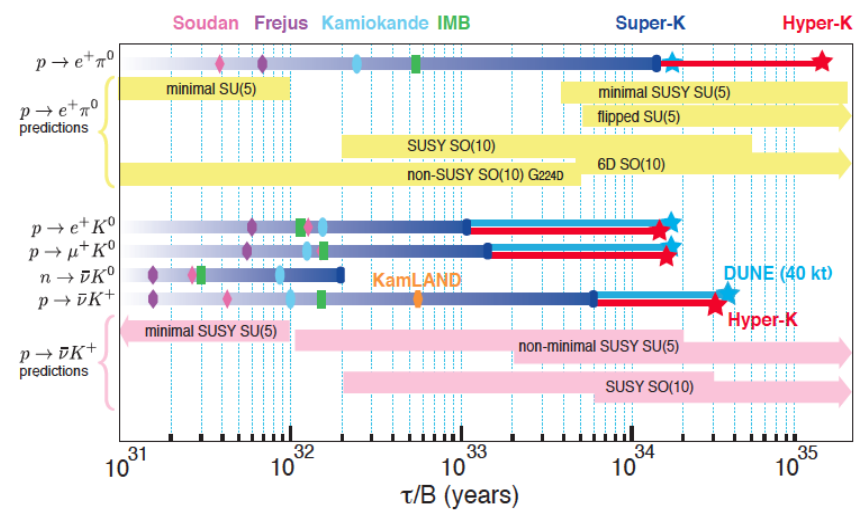
\includegraphics[width=\textwidth]{Chapter-2/Images/PDKExperimentalLImit.png}
\caption{Proton decay lifetime limits from passed and future experiments.}
\label{fig:PDKExperimentalLImit}
\end{figure}


%\subsection{Non-Accelerator Physics Program}
%\subsection{Rare Decay Searches: Experimental Limit}
%\subsection{Nucleon Decay Detection in LAr}
\subsection{Enabling the next generation of discoveries: LArIAT}\label{ch:LArIATIntro}
LArIAT, a small LArTPC in a test beam,  is designed to perform an extensive physics campaign centered on charged particle cross section measurements while characterizing the detector performance for future LArTPCs. Since LArTPCs represent the most advanced experiments for physics at the Intensity Frontier, their complex technology needs a thorough calibration and dedicated measurements of some key quantities to achieve the precision required for the next generation of discoveries.  LArIAT's goal is to provide such calibration and dedicated measurements. The LArIAT LArTPC is deployed in a dedicated calibration test beamline at Fermilab. We use the LArIAT beamline to characterize the charge particles before they enter the TPC: the particle type and initial momentum is known from beamline information. The precise calorimetric energy reconstruction of the LArTPC technology enables the measurement of the total differential cross section for  tagged hadrons. 
The Pion-Nucleus and Kaon-Nucleus total hadronic interaction cross section have never been measured before in argon and they are a fundamental step to shed light on light meson interaction in nuclei per se, while providing a key input to neutrino physics and proton decay studies in future LArTPC experiments like SBN and DUNE. 

In order to showcase LArIAT's utility to SBN and DUNE, we illustrate briefly two comparisons as examples: one regarding neutrino interactions and the second regarding proton decay studies.\\
The left side of figure \ref{fig:NuSimulation} shows the distribution of products in momentum spectrum and particle type as simulated in a $\nu_e$ CC interaction in DUNE (according to \cite{LeiguideOliveira:1953730}); the range of these distribution is to compare with  the momentum distribution of light particles in the LArIAT beamline -- shown on the right side of figure \ref{fig:NuSimulation}. The momentum spectrum in the LArIAT beamline for electrons, muons and pions -- the most abundant particles produced in  a $\nu_e$ CC interaction -- covers a wide range of the expected momentum distribution in a neutrino event.


The signature of a proton decay event in the ``LAr golden mode" is the presence of a single kaon of about 400 MeV in the detector; the momentum spectrum of the kaon pre and post FSI in such an event as simulated by GENIE is shown on the left side of figure \ref{fig:PDKGENIE}. The right side of figure \ref{fig:PDKGENIE} shows the momentum spectrum of kaons in the LArIAT beamline. Kaons arriving to the LArIAT TPC are ideal for proton decay studies, since their momentum in the beamline is just above the typical momentum for kaons in a proton decay event: the majority of LArIAT kaons slow down in the TPC enough to enter the desired momentum window.


\begin{figure}[hbpt]
\centering
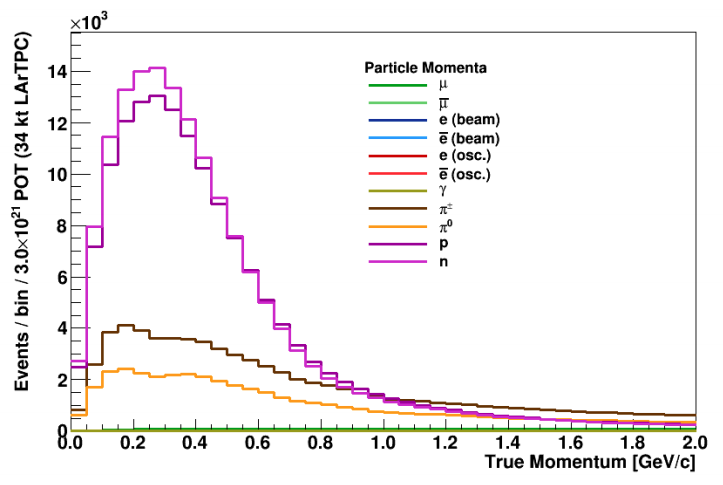
\includegraphics[width=0.45\textwidth]{Chapter-2/Images/NueCCSim.png}	
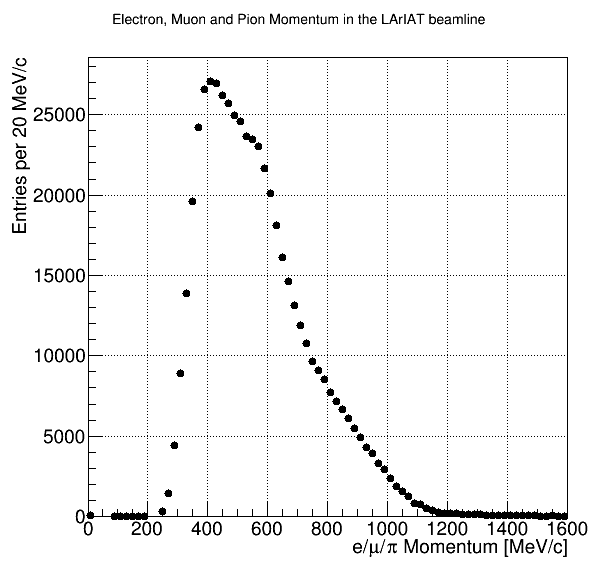
\includegraphics[width=0.45\textwidth]{Chapter-2/Images/momentumPiMuE.png}
\caption{$Left$. Simulation of the products of a $\nu_e$ CC interaction in DUNE, both in particles type and momentum. \\
$Right$. Momentum spectrum for low mass particles ($e,\mu,\pi$) in the LArIAT beamline,  negative tune, Run II, Picky Tracks see section \ref{sec:MWPCfunc}. }
\label{fig:NuSimulation}
\end{figure}


\begin{figure}[hbpt]
\centering
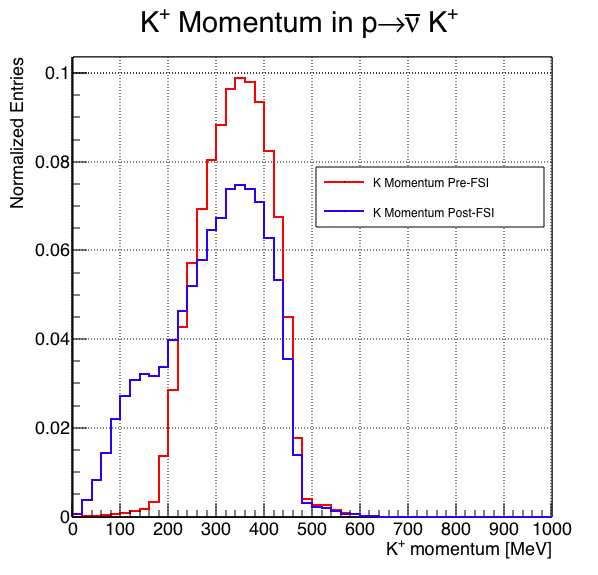
\includegraphics[width=0.45\textwidth]{Chapter-2/Images/pdkGenie.png}	
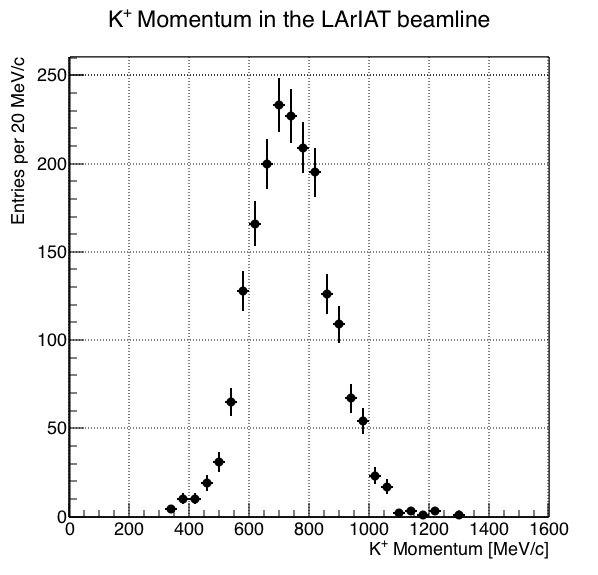
\includegraphics[width=0.45\textwidth]{Chapter-2/Images/MomentumKaonsDatabeamline.png}
\caption{$Left$. Momentum of the kaon outgoing a proton decay $p\rightarrow K^+\bar\nu$ event as simulated by the Genie 2.8.10 event generator in argon. The red line represents the kaon momentum distribution before undergoing the simulated final state interaction inside the argon nucleus, while the blue line represents the momentum distribution after FSI.\\
$Right$. Positive Kaon momentum spectrum in the LArIAT beamline,  positive tune, Run II, Picky Tracks see section \ref{sec:MWPCfunc}. }
\label{fig:PDKGENIE}
\end{figure}



% This chapter to do:
% Re-write the red parts
% write DAQ part
% re-write captions
% put references
% re-read

\chapter{LArIAT: Liquid Argon In A Testbeam}\label{sec:experimentDescription}
In this chapter, we describe the LArIAT experimental setup. We start by illustrating the journey of the charge particles in the Fermilab accelerator complex, from the gaseous thermal hydrogen at the Fermilab ion source to the delivery of the LArIAT tertiary beam at MC7. We  then describe the LArIAT beamline detectors, the LArTPC, the DAQ and the monitoring system.

%\section{LArIAT \& the Intensity Frontier}
\section{The Particles Path to LArIAT}

LArIAT's particles history begins in the Fermilab accelerator complex with a beam of protons. The process of protons acceleration develops in gradual stages (see picture \ref{fig:Accelerator}): gaseous hydrogen is ionized in order to form H$^{-}$ ions; these ions are boosted to 750 keV by a Cockroft-Walton accelerator and injected to the Linac linear accelerator that increases their energy up to 400 MeV; then, H$^{-}$ ions pass through a carbon foil and lose the two electrons; the resulting protons are then injected into a rapid cycling synchrotron, called Booster; at this stage, protons reach 8 GeV of energy and are compacted into bunches; the next stage of acceleration is the Main Injector, a synchrotron which accelerates the bunches up to 120 GeV; in the Main Injector, several bunches are merged into one and used for the injection in the last stage.


The Fermilab accelerator complex works in supercycles of roughly 60 seconds in duration. The beam is split by electrostatic septa and delivered at different experimental halls all over the lab. A 120~GeV$/c$ primary proton beam with variable intensity is extracted in four-second ``spills" and sent to the Meson Center beam line. 

LArIAT's home at Fermilab is the Fermilab Test Beam Facility (FTBF), where the experiment characterizes a beam of charge particles downstream from the Meson Center beam line. 
Here, the primary beam is focused onto a tungsten target to create LArIAT's secondary beam. The composition of the secondary particle beam is mainly positive pions. The momentum peak of the secondary beam was fixed at 64~GeV/c for the LArIAT data considered in this work, although the beam is tunable in momentum between 8-80\,GeV/c; this configuration of the secondary beamline assured a stable beam delivery at the LArIAT experimental hall.
 
The secondary beam impinges then on a copper target within a steel collimator inside the LArIAT experimental hall (MC7) to create the LArIAT tertiary beam, (shown in  Fig.~\ref{fig:tert-layout}).   The steel collimator selects particles produced with a $13^\circ$ production angle at the target down the beamline.  The particles are then bent by  $~10^\circ$  through a pair of dipole magnets.  By configuring the field intensity of the magnets we allow the particles of LArIAT's tertiary beam to span a momentum range from 0.2 to 1.4~GeV/c. The polarity of the magnet is also configurable and determines the sign of the beamline particles which are focused on the LArTPC. If the magnets polarity is positive the tertiary beam composition counts mostly pions and protons with a small fraction of electrons, muons, and kaons. It is the job of the LArIAT beamline detectors to select the particles polarity,  to perform particle identification in the beamline and to measure the momentum of the tertiary beam particles before they get to the LArTPC. The LArIAT detectors are described in the following paragraphs.  



%\begin{comment}     
\begin{figure}
  \centering  	
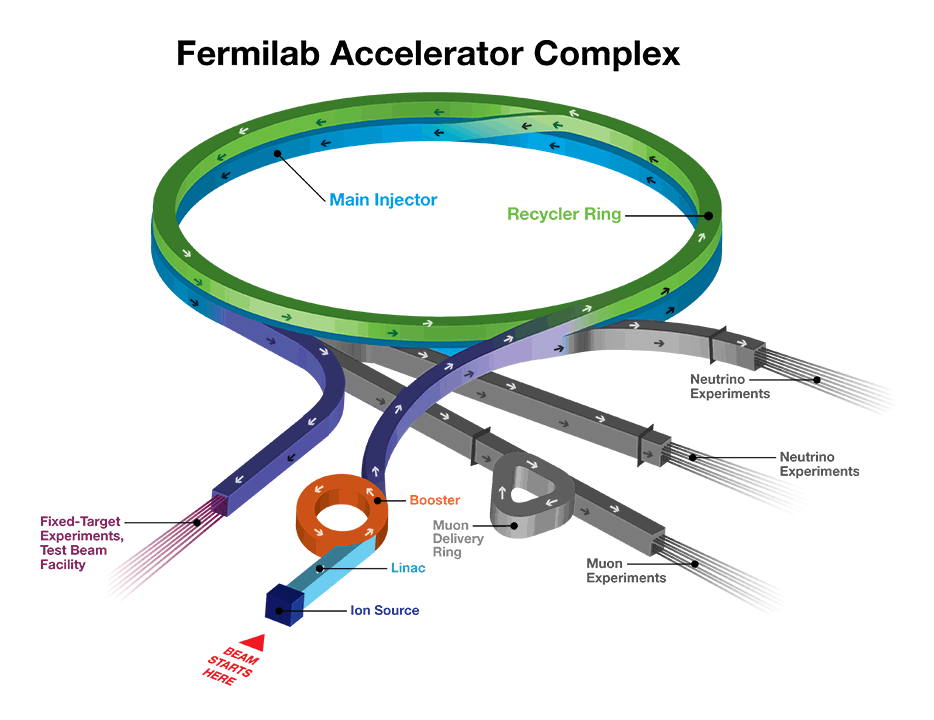
\includegraphics[width=\textwidth,height=\textheight,keepaspectratio]{Chapter-3/Images/AcceleratorFNAL.png}
\caption{Layout of Fermilab Acellerator complex.}
\label{fig:Accelerator}
\end{figure}

%\begin{comment}     
\begin{figure}
  \centering  	
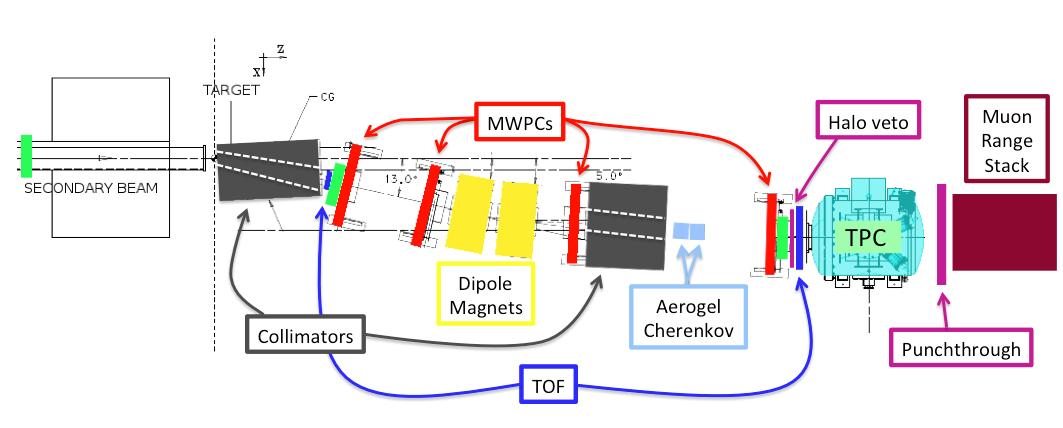
\includegraphics[width=\textwidth,height=\textheight,keepaspectratio]{Chapter-3/Images/Tertiary.png}
\caption{Bird's eye view of the LArIAT tertiary beamline. In grey: upstream and downstream collimators; in yellow: bending magnets; in red: wire chambers; in blue: time of flight; in green: liquid argon TPC volume; in maroon: muon range statck.}
\label{fig:tert-layout}
\end{figure}


%%%%%%%%%%%%%%%%%%%%%%%%%%%%%%%%%%%%%%%%%%%%%%%%%%%%%%%%%%%%
\section{LArIAT Tertiary Beam Instrumentation}\label{sec:Instrumentation}

%%%%%%%%%%%%%%%%%%%%%%%%%%%%%%%%%%%%%%%%%%%%%%%%%%%%%%%%%%%%
The instrumentation of  LArIAT tertiary beam and the TPC components have changed several times during the three years of LArIAT data taking. The following paragraphs describe the components operational during ``Run II", the data taking period relevant to the hadron cross section measurements.

The key components of the tertiary beamline instrumentation for the hadron cross section analyses are the two bending magnets, a set of four wire chambers (WCs) and two time-of-flight scintillating paddles (TOF) and, of course, the LArTPC.  The magnets determine the polarity of the particles in the tertiary beam; the combination of magnets and wire chambers determines the particles' momentum, which is used to determine the particle species in conjunction with the TOF.
A muon range stack downstream from the TPC and two sets of cosmic paddles configured as a telescope surrounding the TPC are also used for calibration purposes.


\subsection{Bending Magnets}\label{sec:Magnets}
%%%%%%%%%%%%%%%%%%%%%%%%%%%%%%%%%%%%%%%%%%%%%%%%%%%%%%%%%%%

LArIAT uses a pair of identical Fermilab type ``NDB" electromagnets, recycled from the Tevatron's anti-proton ring, in a similar configuration used for the  MINERvA T-977 test beam calibration~\cite{MinervaTestbeam}). 
The magnets are a fundamental piece of the LArIAT beamline equipment, as they are used for both particle identification and momentum measurement before the LArTPC. The sign of the current in the magnets allows us to select either positively or negatively charged particles; the value of the magnetic field is used in the momentum determination and in the subsequent particle identification. 

We describe here the characteristics and response of one magnet, as the second one has a similar response, given its identical shape and history. Each magnet is a box with a rectangular aperture gap in the center to allow for the particle passage.  The magnet aperture measures 14.224~cm in height, 31.75~cm in width, and  46.67~cm in length.  Since the wire chambers aperture ($\sim$12.8~cm$^2$) is smaller than the magnet aperture, only the central part of the magnet gap is utilized. The field is extremely uniform over this limited aperture and was measured with two hall probes, both calibrated with nuclear magnetic resonance probes. The probes measured the excitation curve shown in Figure~\ref{fig:magnet_excitation}. 

\begin{figure}[!h]
\begin{centering}
\vspace{-0.3cm}
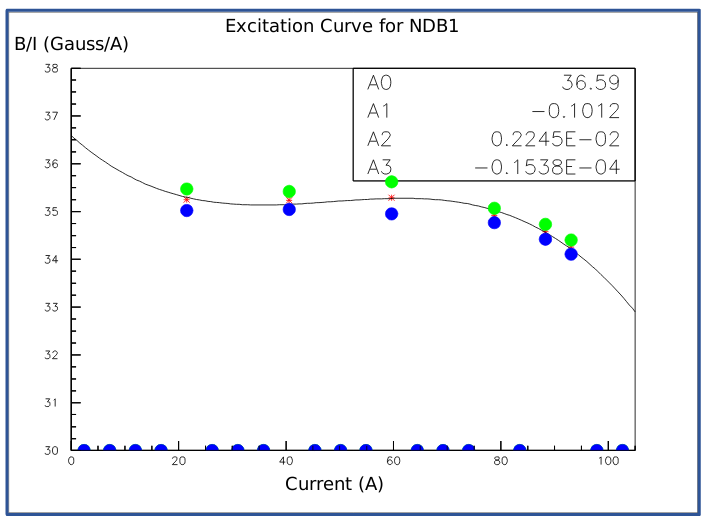
\includegraphics[height=3.0in]{Chapter-3/Images/ExcitationCurves.png}
\caption{
{ Magnetic field over current as a function of the current, for one NDB magnet (excitation curve). The data was collected using two hall probes (blue and green). We fit the readings with a cubic function (black) to average of measurements (red) given in the legend.}
}
\label{fig:magnet_excitation}
\end{centering}
\end{figure}

The current through the magnets at a given time is identical in both magnets. For the Run II data taking period, the current settings explored were 60A (B $\sim$0.21 T) and 100A (B $\sim$0.35 T) in both polarities. 
Albeit advantageous to enrich the tertiary beam composition with high mass particles such as kaons, we never pushed the magnets current over 100 A, not to incur in overheating.  During operation, we operated a air and water cooling system on the magnets and we remotely monitored the magnets temperature.
 
\subsection{Multi-Wire Proportional Chambers}\label{sec:MWPC}
%%%%%%%%%%%%%%%%%%%%%%%%%%%%%%%%%%%%%%%%%%%%%%%%%%%%%%%%%%%%
\begin{figure}[!h]
\begin{centering}
\vspace{-0.3cm}
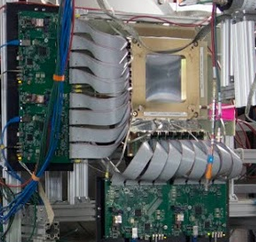
\includegraphics[height=2.3in]{Chapter-3/Images/WireChamber.png}
\caption{
{One of the four Multi Wire Proportional Chambers (WC) used in the LArIAT tertiary beamline and relative read-out electronics.}
}
\label{fig:wirechamber}
\end{centering}
\end{figure}

LArIAT uses four multi-wire proportional chambers, or wire chambers (WC) for short, two upstream and two downstream from the bending magnets. The geometry of one chamber is shown in Figure~\ref{fig:wirechamber}: the WC effective aperture is a square of  12.8~cm perpendicular to the beam direction.  Inside the chamber, the 128 horizontal and 128 vertical wires hang at a distance of 1~mm from each other in a mixture of 85\% Argon and 15\% isobutane gas.  The WC operating voltage is between 2400~V and 2500~V. The LArIAT wire chambers are an upgraded version of the Fenker Chambers~\cite{Fenker}, where an extra grounding improves the signal to noise ratio of the electronic readout.  

Two ASDQ chips~\cite{ASDQchip} mounted on a mother board plugged into the chamber serve as front end amplifier/discriminator. The chips are connected to a multi-hit TDC~\cite{Sten} which provides a fast OR output used as first level trigger. The TDC time resolution is 1.18~ns/bin and can accept 2 edges per 9~ns.  
The maximum event rate acceptable by the chamber system is of 1 MHz: this rate is not a limiting factor considering that \textcolor{red}{the rate of the tertiary particle beam at the first wire chamber is estimated to be less than 15 kHz}. A full spill of data occurring once per supercycle is stored on the TDC board memory at once and read out by a specially designed controller.  We use LVDS cables to carry both power and data between the controller and the TDCs and from the controller to the rest of the DAQ.  
%It is possible to program the time window for acceptance for hits, time offsets, front end threshold, and pulse shaping parameters through the controller via a USB from a PC or through an Ethernet connection.

\subsubsection{Multi-Wire Proportional Chambers functionality}\label{sec:MWPCfunc}
We use the wire chamber system together with the bending magnets to measure the particle's momentum.

In the simplest scenario, only one hit on each and every of the four wire chambers is recorded during a single readout of the detector systems.  Thus, we use the hit positions in the two wire chambers upstream of the magnets to form a trajectory before the bend, and the hit positions in the two wire chambers downstream of the magnets to form a trajectory after the bend. We use the angles in the XZ plane between the upstream and downstream trajectories  to calculate the $Z$ component of the momentum as follows:

\begin{equation}
P_z=\frac{B_{eff}L_{eff}}{3.3(sin(\theta_{DS})-sin(\theta_{US}))},
\label{eq:momformula}
\end{equation}

where $B_{eff}$ is the effective maximum field in a square field approximation,  $L_{eff}$ is the effective length of both magnets (twice the effective length of one magnet), $\theta_{US}$ is the angle off the $z$ axis of the upstream trajectory, $\theta_{DS}$ is the angle off the $z$ axis of the downstream trajectory  and  3.3~$c^{-1}$ is the conversion factor from [T$\cdot$m] to [MeV/c]. By using the hit positions on the third and fourth wire chamber, we estimate the azimutal and polar angles of the particle trajectory, and we are able to calculate the other components of the momentum. 

The presence of multiple hits in a single wire chamber or the absence of hits in one (or more) wire chambers can complicate this simple scenario. The first complication is due to beam pile up, while the latter is due to wire chamber inefficiency. In the case of multiple hits on a single WC, at most one wire chamber track is reconstructed per event. Since the magnets bend particles only in the X direction, we assume the particle trajectory to be roughly constant in the YZ plane, thus we keep the combination of hits which fit best with a straight line. 
It is still possible to reconstruct the particle's momentum  even if the information is missing in either of the two middle wire chambers (WC2 or WC3), by constraining the particle trajectory to cross the plane in between the magnets. 
%Under the assumption of identical magnets, we define a plane centered in the middle of the two magnets (called ``midplane") that the physical particles need to cross. We project the completed half of the wire chamber track to the midplane, assuming no bending, to find the point of intersection. We use this point to complete the other half of the wire chamber track and to calculate the reconstructed momentum  with these four points. To account for the lack of bending in our reconstructed wire chamber track, we apply to the calculated momentum  a correction obtained with a sample of 4-point, single hit tracks.

Events satisfying the simplest scenario of one single hit in each of the four wire chambers form the ``Picky Track" sample.  We construct another, higher statistics sample, where we loosen the requirements on single hit and wire chamber efficiency: the ``High Yield" sample. For LArIAT Run II, the High Yield sample is about three times the Picky Tracks statistics.  For the first measurements of the LArIAT hadronic cross section, we use the Picky Tracks sample because the uncertainty on the momentum is smaller and the comparison with the beamline MC results is straightforward compared with the High Yield sample;  a possible future update and cross check of these analysis would be the use of the High Yield sample. 

%We use Picky Tracks to calibrate the momentum measurement for the High Yield sample, in particular to obtain a momentum correction for  tracks missing information from the central WCs;  this correction adds an uncertainty of approximately 2\% to the momentum calculation of the High Yield sample.

\textcolor{red}{Four point track momentum uncertainty}

\subsection{Time-of-Flight System}\label{sec:TOF}
%%%%%%%%%%%%%%%%%%%%%%%%%%%%%%%%%%%%%%%%%%%%%%%%%%%%%%%%%%%%
Two scintillator paddles, one upstream to the first set of WCs and one downstream to the second set of WCs  form LArIAT  time-of-flight (TOF) detector system. 

The upstream paddle is made of a 10 x 6 x 1~cm scintillator piece, read out by two PMTs mounted on the beam left side which collect the light from light guides mounted on all four edges of the scintillator. The downstream paddle is a   14 x 14 x 1~cm scintillator piece read out by two PMTs on the opposite ends of the scintillator.
The relatively thin width on the beamline direction minimizes energy loss of the particles coming from the target in the scintillator material.

The CAEN 1751 digitizer is used to digitize the TOF PMTs signals at a sampling rate of 1 GHz. The 12 bit samples are stored in a circular memory buffer. At trigger time, data from the TOF PMTs are recorded to output in a 28.7 \textmu s windows starting  approximately 8.4 \textmu s before the trigger time. 



\subsubsection{TOF functionality}\label{sec:MWPCfunc}


The TOF signals rise time (10-90\%) is 4 ns and a full width, half-maximum of 9 ns consistent in time. The signal amplitudes from the upstream TOF and  downstream TOF are slightly different:  200 mV for the upstream PMTs but only 50 mV for downstream PMTs. The time of the pulses was calculated utilizing an oversampled template derived from the data itself. We take the pulse pedestal from samples far from the pulse and subtract it to the pulse amplitude. We then stretch vertically a template to match the pedestal-subtracted pulse amplitude and we move it horizontally to find the time. With this technique, we find a pulse time-pickoff resolution better than 100 ps.  The pulse pile up is not a significant problem given the TOF timing resolution and the rate of the particle beam.  Leveraging on the pulses width uniformity of any given PMT,  we flag events where two pulses overlap as closely in time as 4 ns with an 90\% efficiency according to simulation. 


We combine the pulses from the two PMTs on each paddle to determine the particles' arrival time by averaging the time measured from the single PMT, so to minimize errors due to optical path differences in the scintillator.  However, a time spread of approximately 300~ps is present in both the upstream and downstream detectors, likely due to transit time jitter in the PMTs themselves.  There is no evidence of systematic timing drift over long data-taking periods such as 3-4 months: the maximum variation of the average time differences between pairs of PMTs reading out the same scintillator is of the order of 150~ps.

\begin{figure}[h!]
\centering
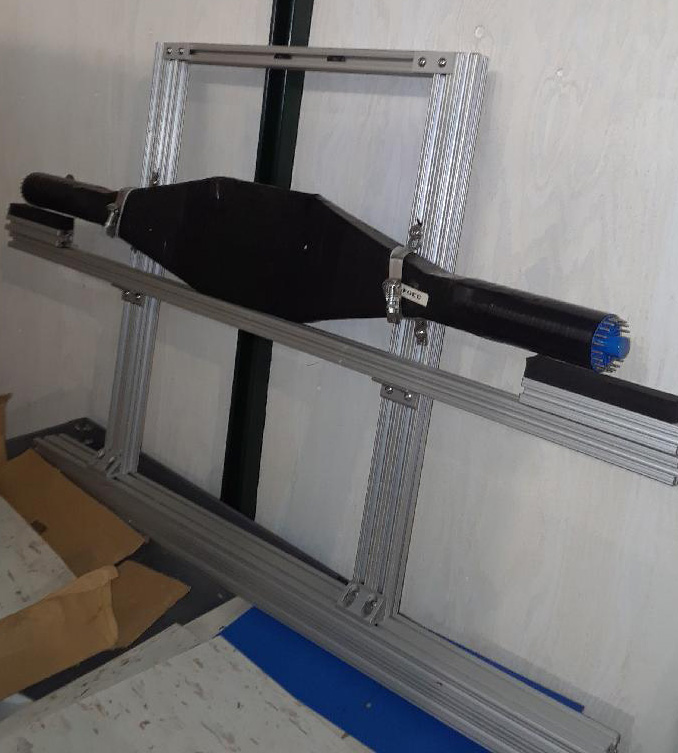
\includegraphics[width=0.5\textwidth]{Chapter-3/Images/DSTOF.jpg}
\caption{Image of the down stream time of flight paddle, PMTs and relative support structure before mounting. } 
\label{pic:cosmicpaddle}
\end{figure}


%\textcolor{red}{calculated TOF with error}


%%%%%%%%%%%%%%%%%%%%%%%%%%%%%%%%%%%%%%%%%%%%%%%%%%%%%%%%%%%%
\subsection{Punch-Through and Muon Range Stack Instruments}\label{sec:MuRS}
%%%%%%%%%%%%%%%%%%%%%%%%%%%%%%%%%%%%%%%%%%%%%%%%%%%%%%%%%%%%

The punch-thorough and the muon range stack (MuRS) detectors are located downstream of the TPC. These detectors provide a sample of  TPC crossing tracks without relying on TPC information and can be used to improve particle ID for  muons and pions with momentum higher than  450 MeV/c.

The punch-thorough is simple sheet of scintillator material, read out by two PMTs. 
The MuRS is a segmented block of steel with four slots instrumented with scintillation bars. The four steel layers in front of each instrumented slot are 2 cm, 2 cm, 14 cm and 16 cm wide in the beam direction. Each instrumented slot is equipped with four scintillation bars each, positioned horizontally in the direction orthogonal to the beam. Each scintillator bar measures  \textcolor{red}{? x ? x 2}~cm and it is read out by one PMT.  

The signals from both the punch-thorough and the MuRS PMTs are digitized in the CAEN V1740, same as the TPC; the details of this discriminator are laid out in~\ref{sec:TPCCharge}. It is worth noticing that the sampling time of the CAEN V1740 is slow (of the order of 128 ns), so pulse shape information from the PMT is lost.
Punch-thorough and MuRS hits are formed utilizing the digital discriminator signals under threshold at a given time, where we obtain the threshold for each PMT directly on data distributions.



%%%%%%%%%%%%%%%%%%%%%%%%%%%%%%%%%%%%%%%%%%%%%%%%%%%%%%%%%%%%
\subsection{LArIAT Cosmic Ray Paddle Detectors}\label{sec:CosmicRayPaddle}
%%%%%%%%%%%%%%%%%%%%%%%%%%%%%%%%%%%%%%%%%%%%%%%%%%%%%%%%%%%%
LArIAT triggers both on beam events and on cosmic rays events. We perform this latter trigger by using two sets of cosmic ray paddle detectors (a.k.a. ``cosmic towers".) The cosmic towers frame the LArIAT cryostat, as one sits in the downstream left corner and the other sits in the upstream right corner of the cryostat. Two paddle sets of four scintillators pieces each make up each cosmic tower, an upper set and a lower set per tower. 
Of the four paddles, a couple of two matched paddles stands upright while the a second matched pair lies across the top of the assembly in the top sets (or across the bottom of the assembly in the bottom sets). The horizontal couple is used as a veto for particles traveling from inside the TPC out.  The four signals  from the vertical paddles along one of the body diagonals of the TPC are combined in a logical ``AND''. This allows to select cosmic muons crossing the TPC along one of its diagonals.  Cosmic ray tracks crossing both anode and cathode populate the events triggered this way. This particularly useful sample of tracks (which we can safely assume to be associated with ~5 GeV muons) can be used for many tasks; for example, we use anode-cathode piercing tracks to cross check the TPC electric field on data (see Appendix \ref{ch:AppendixB}), to calibrate the charge response of the TPC wires for the full TPC volume and to measure the electron lifetime in the chamber (see section \ref{ch:EnCalibration})\textcolor{red}{ ADD pictures}.

%%%%%%%%%%%%%%%%%%%%%%%%%%%%%%%%%%%%
%All the paddles are 3.02~cm thick and are  trapezoidal in shape. The paddles come in two sizes: the smaller version has bases 32.2~cm and 26.7~cm, and 61.0~cm height, while the bigger version has bases 33.2~cm and 27.0~cm, and $70.8~cm$ height. 
 A Zener-diode Hamamatsu H5783 PMT collects the light from a wavelength-shifting optical fiber which runs along one of the long sides of each paddle. A custom-made PMT Amplifier and Discrimination (PAD) circuit mounted at one end of the paddle collects signals from the PMTs and sends them to the Control and Concentrator Unit (CCU). We use the same connection to  power the PMT, control voltage and threshold, and output the PMT signal as logic ECL pulse.
We retrieved the scintillation paddles from the decommissioning of the CDF detector at Fermilab and we used only the paddles with a counting efficiency greater than 95\% and low noise at working voltage. The measured trigger rate of the whole system is 0.032~Hz, corresponding to $\sim 2$ muons per minute.


\begin{figure}[h!]
\centering
 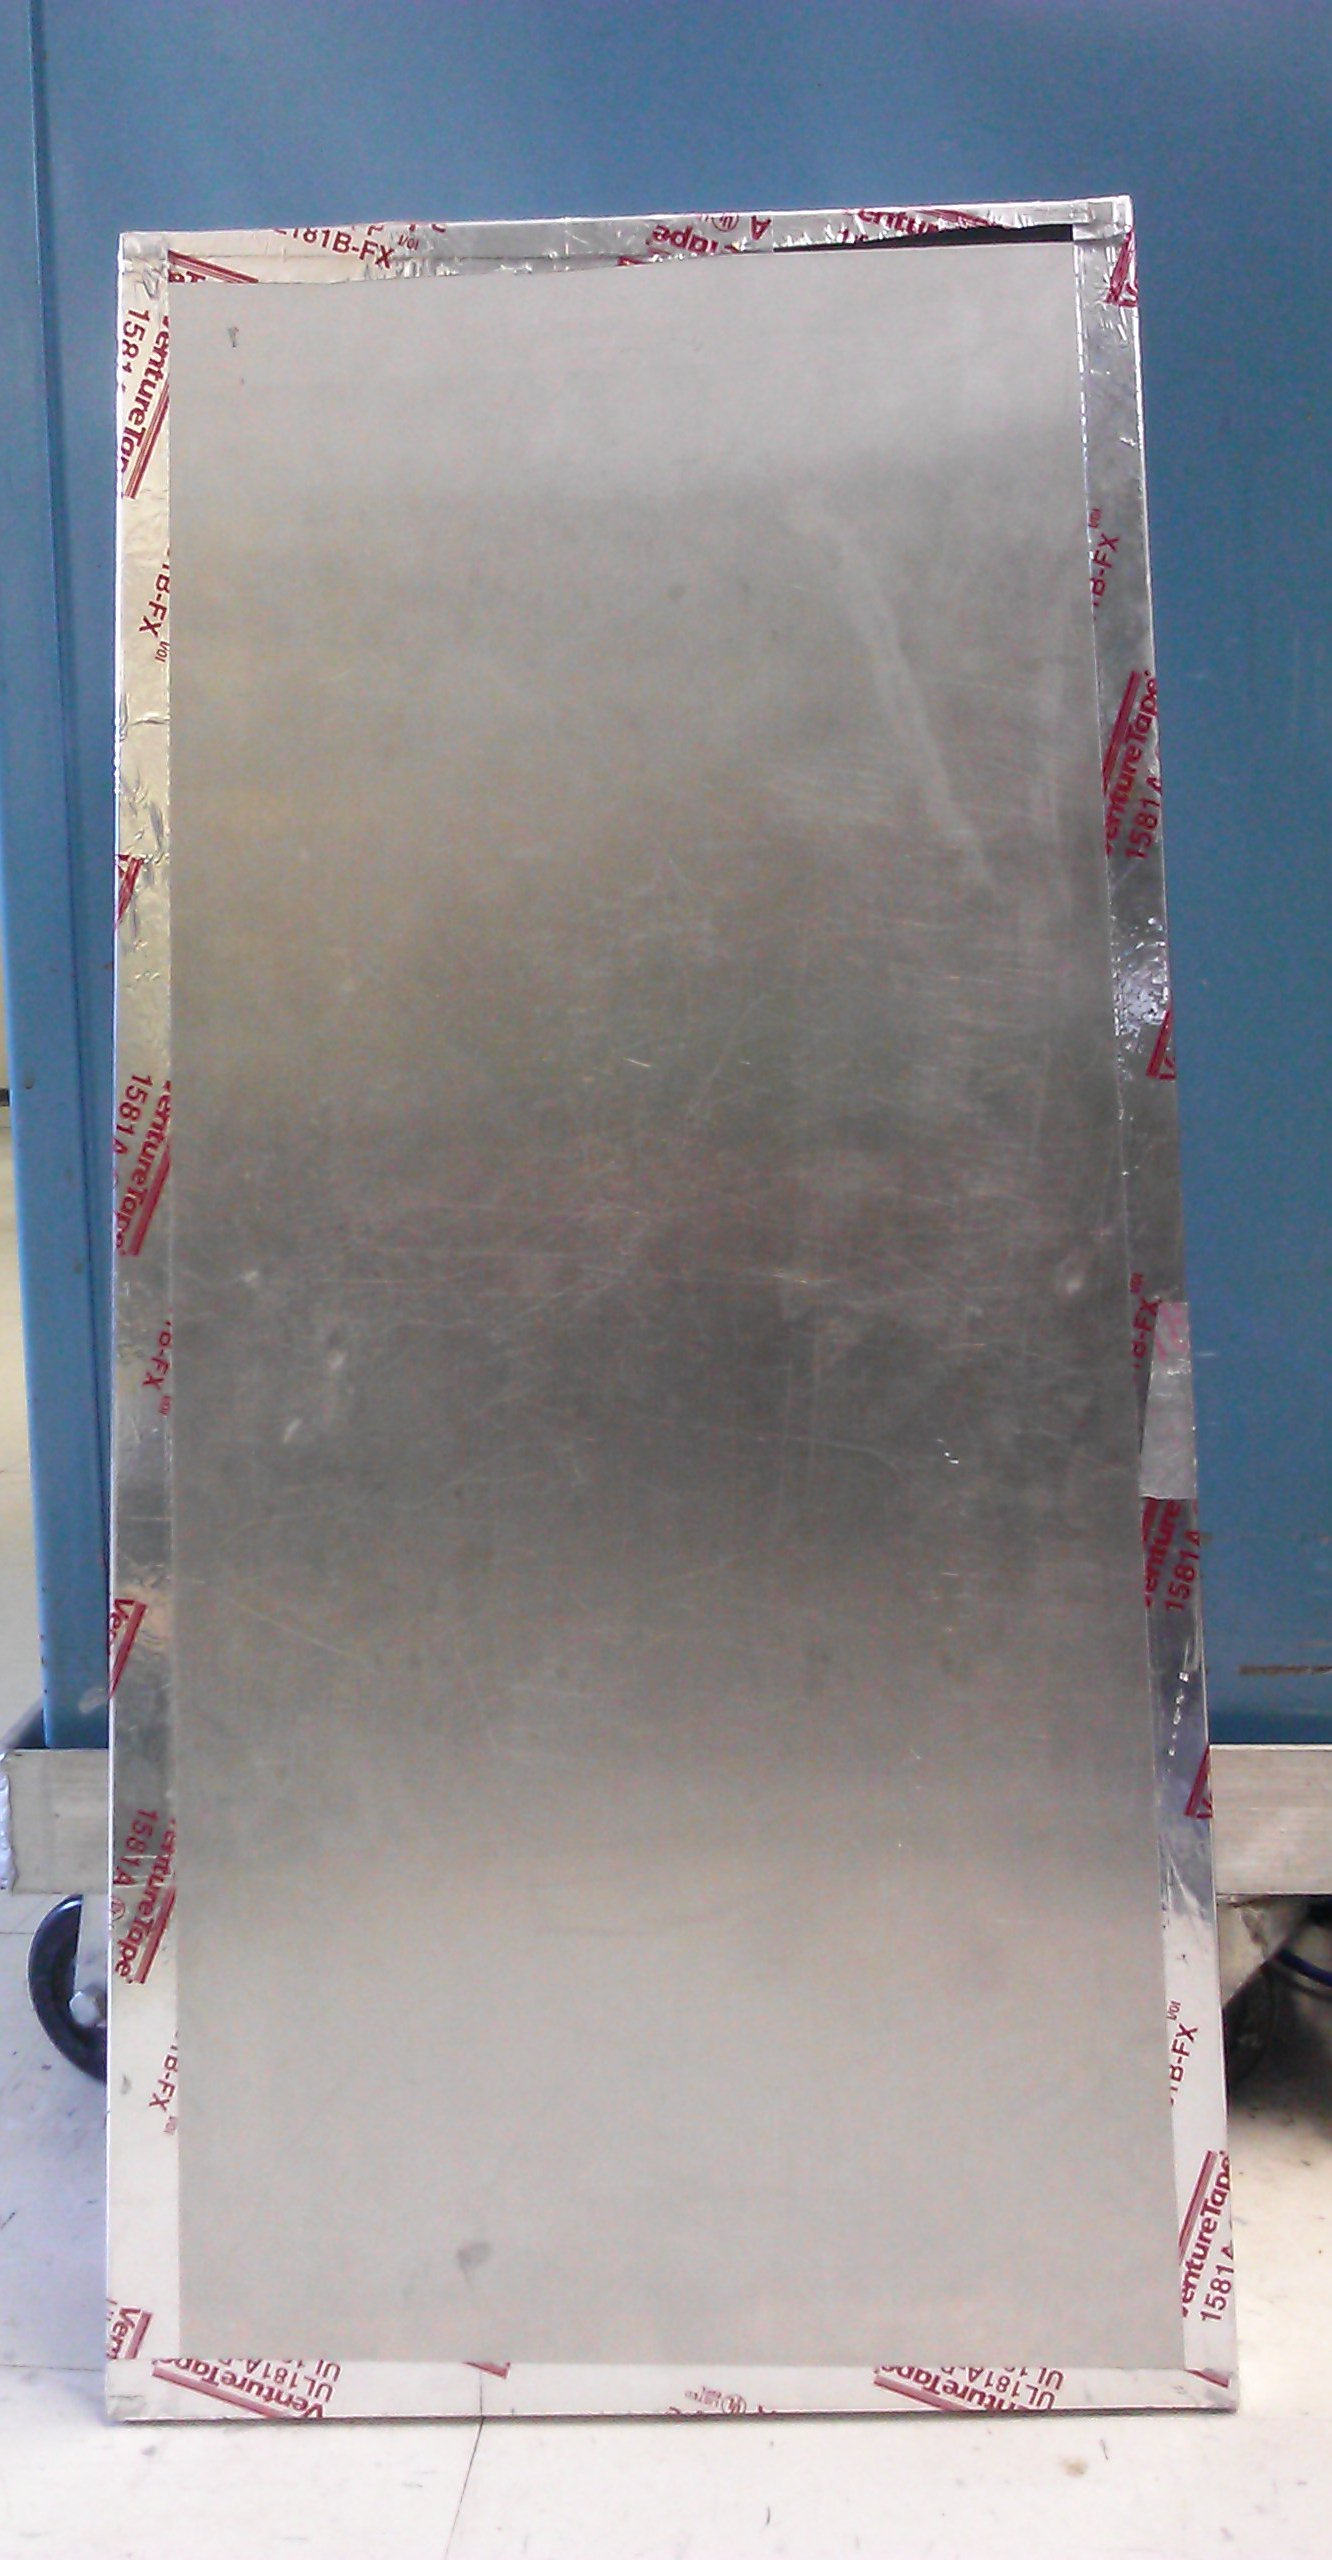
\includegraphics[angle=90,width=0.7\textwidth]{Chapter-3/Images/Cosmic_Paddle.jpg}
\caption{Photograph of one of the scintillation counters used in the cosmic towers. } 
\label{pic:cosmicpaddle}
\end{figure}





\section{In the Cryostat}
\subsection{Cryogenics and Argon Purity}\label{ch:Cryo}
LArIAT repurposed the ArgoNeuT cryostat \cite{ArgoNeuT-det} in order to use it in a beam of charge particles, and added a new process piping and a new liquid argon filtration system in FTBF.  %The main modifications to the ArgoNeuT cryostat are the addition of a beam flange and a port for the light collection system, 
Inside the LArIAT experimental hall, the cryostat sits on the beam of charge particles with its horizontal main axis oriented parallel to the beam.

Two volumes make up LArIAT cryostat, shown in Figure \ref{fig:LArIATCryoStat}:  the inner vessel and the outer vessel. Purified liquid argon fills the inner vessel, while the outer volume provides insulation through a vacuum jacket equipped with layers of aluminized mylar superinsulation. The inner vessel is a cylinder of 130~cm length and 6.2~cm diameter, containing about 550~L of LAr, corresponding to a mass of 0.76 ton. We run the signal cables for the LArTPC and the high voltage feedthrough through a ``chimney'' at the top and mid-length of the cryostat.


\begin{figure}[htb]
\centering
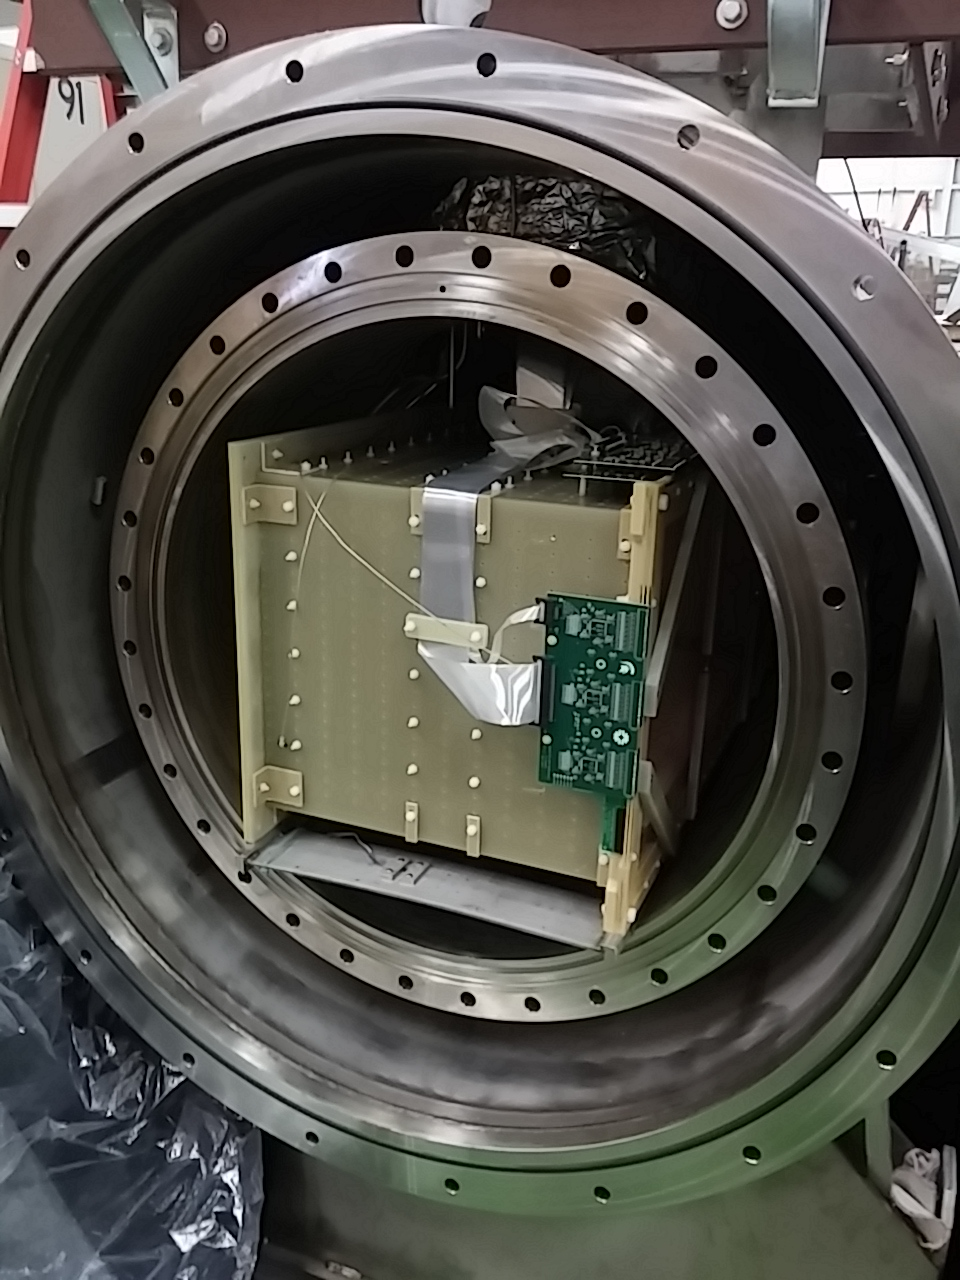
\includegraphics[scale=0.18]{Chapter-3/Images/Cryostat1.jpg}
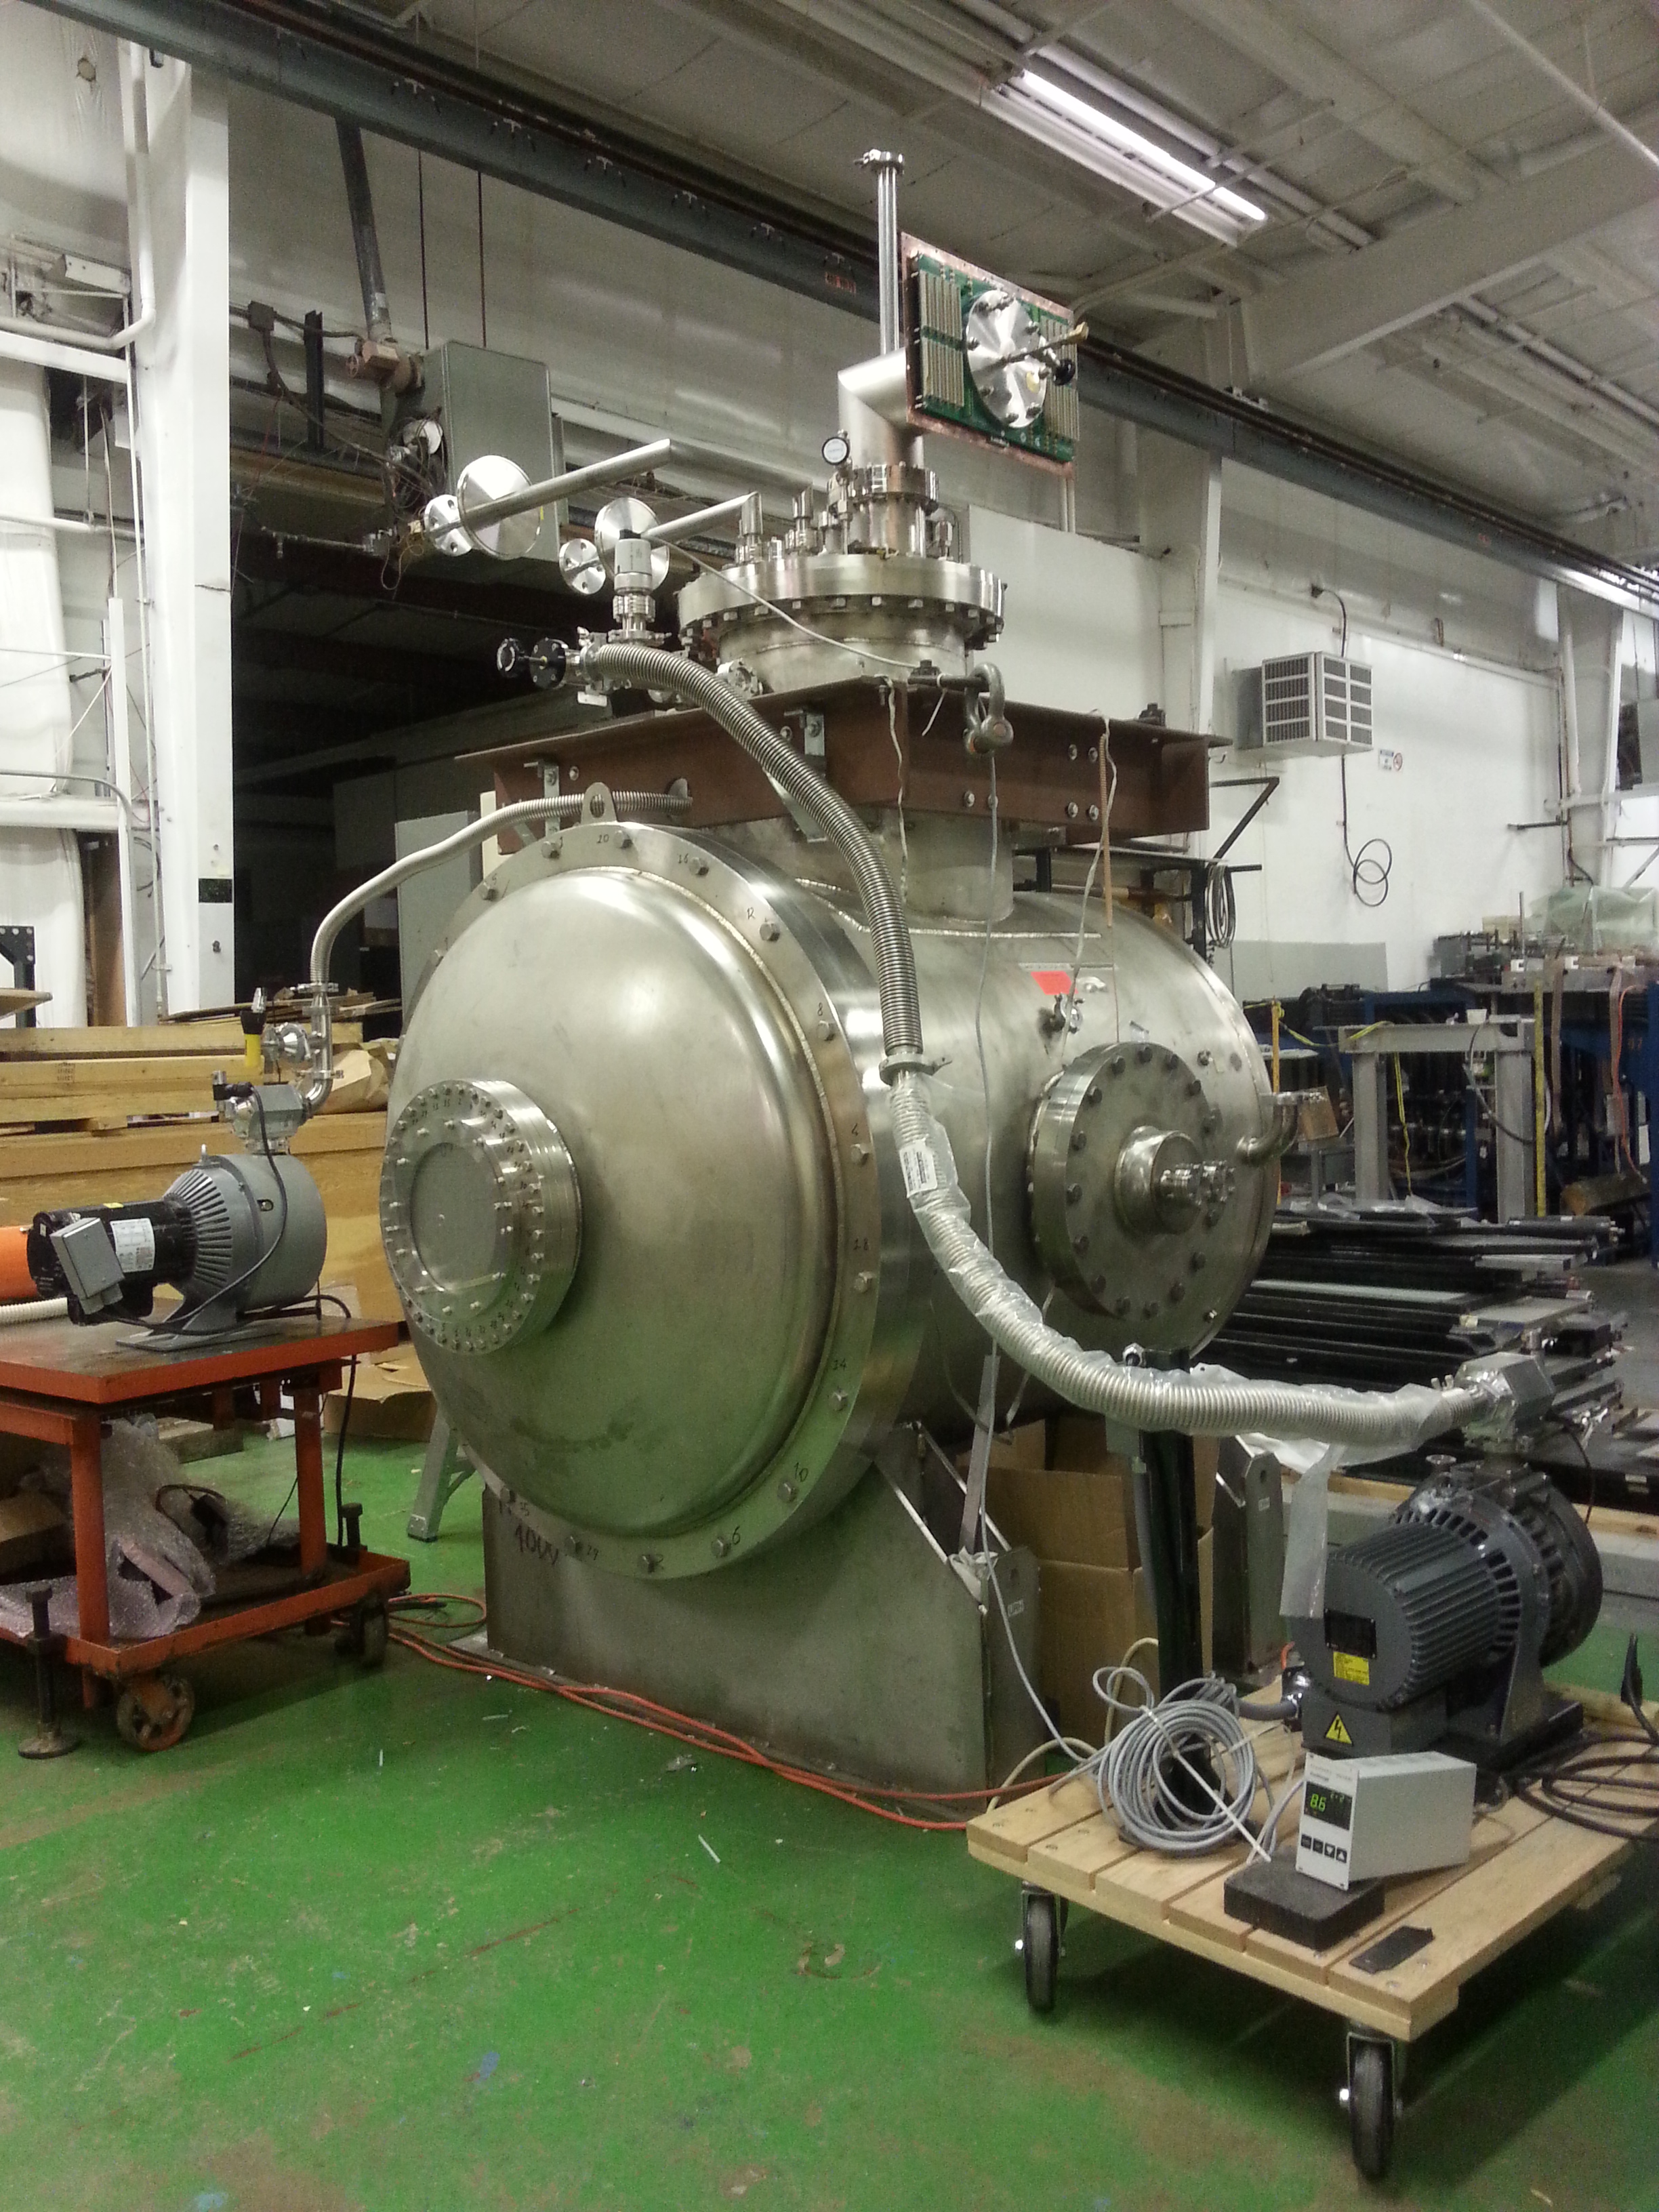
\includegraphics[scale=0.07]{Chapter-3/Images/Cryostat2.jpg}
\caption{ Left: the LArIAT TPC in the inner volume of the open cryostat. Right: cryostat fully sealed ready to be transported to FTBF. }
\label{fig:LArIATCryoStat}
\end{figure}

Given the different scopes of the ArgoNeuT and LArIAT detectors, we made several modification to the ArgoNeuT cryostat in order to use it in LArIAT. In particular, the modification  shown in Figure \ref{fig:LArIATCryoMods} were necessary to account for the beam of charged particles entering the TPC and to employ the new FTBT liquid argon purification system. 
We added a ``beam window'' on the front outer end cap and an ``excluder'' on the inner endcap, with the scope of minimizing the amount of dead material upstream of the TPC's active volume.  Doing so, we reduced the amount of uninstrumented material before the TPC from $\sim$ 1.6 radiation lengths ($X_{0}$) (ArgoNeuT) to less than 0.3 $X_{0}$ (LArIAT). To allow studies of the scintillation light, we added a side port feedthrough which enables the mounting of the light collection system, as well as the connections for the corresponding signal and high-voltage cables (see Section \ref{sec:TPCLight}).  We modified the bottom of the cryostat adding Conflat and ISO flange sealing to connect the liquid argon transfer line to the new argon cooling and purification system.


\begin{figure}[htb]
\centering
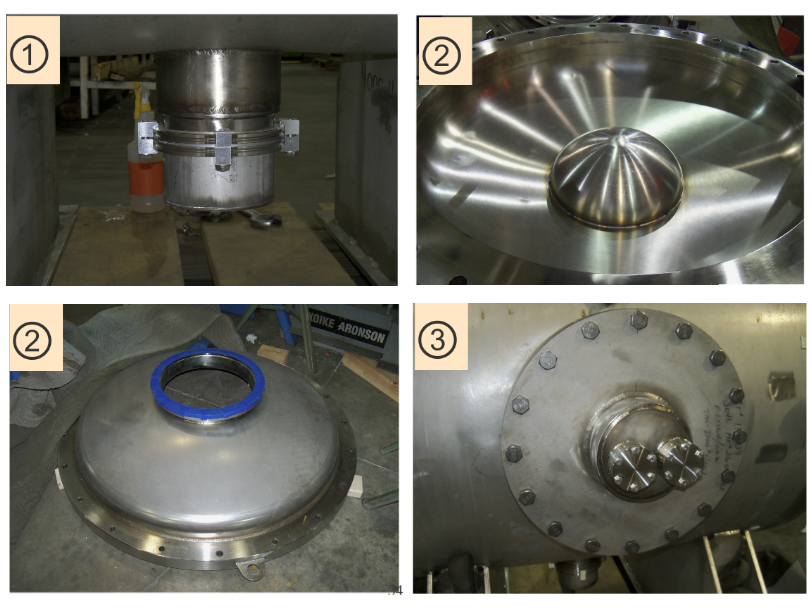
\includegraphics[scale=0.35]{Chapter-3/Images/CryoMods.png}
\caption{Main modifications to the ArgoNeuT cryostat: $1)$ outlet for connection to the purification system at the bottom of the cryostat; $2)$ the ``beam-window'' on the outer endcap and ``excluder"  which reduce the amount of non-instrumented material before the TPC; $3)$ the side port to host  the  light collection system.}
\label{fig:LArIATCryoMods}
\end{figure}

%%%%%%%%%%%%%%%%%%%%%
As in any other LArTPC, argon purity is a crucial parameter for LArIAT. Indeed, the presence of contaminants effects both the basic working principles of a LArTPC: electronegative contaminants such as oxygen and water decrease the number of ionization electrons collected on the wires after drifting through the volume, while contaminants such as Nitrogen decrease the light yield from scintillation light, especially in its slow component.
In LArIAT, contaminations should not exceed the level of 100 parts per trillion (ppt). We achieve this level of purity in several stages. The specifics required for the commercial argon bought for LArIAT are 2 parts per million (ppm) oxygen, 3.5~ppm water, and 10~ppm nitrogen. This argon is monitored with the use of commercial gas analyzer.
Argon is stored in a dewar external to LArIAT hall and filtered before filling the TPC. %The argon is delivered from the commercial dewar to the cryostat through 2.54~cm diameter schedule 10 stainless steel piping.  The piping was insulated with 20.32~cm of polyurethane foam by the manufacturer.  The piping was cleaned to remove oil and grease before being welded into the system. 
LArIAT uses a filtration system designed for the Liquid Argon Purity Demonstrator (LAPD)~\cite{LAPD}: half of a 77~liter filter contains a 4A molecular sieve (Sigma-Aldrich~\cite{sigma-aldrich}) apt to remove mainly water, while the other half contains BASF~CU-0226~S, a highly dispersed copper oxide impregnated on a high surface area alumina, apt to remove mainly oxygen~\cite{basf}. A single pass of argon in the filter is sufficient to achieve the necessary purity, unless the filter is saturated. In case the filter saturates, the media needs to be regenerated by using heated gas; this happened twice during the Run II period\footnote{We deemed the filter regeneration necessary every time the electron lifetime dropped under 100 \textmu s.}.
The filtered argon reaches the inner vessel via a liquid feedthrough on the top of the cryostat. Argon is not recirculated in the system, rather it boils off and vent to the atmosphere. During data taking, we replenish the argon in the cryostat several times per day to keep the TPC high voltage feedthrough and cold electronics always submerged. In fact, we constantly monitor the level, temperature, and pressure of the argon both in the commercial dewar and inside the cryostat during data taking. 
\subsection{LArTPC: Charge Collection}\label{sec:TPCCharge}
The LArIAT Liquid Argon Time Projection Chamber is a rectangular box of dimensions 47 cm (width) x 40 cm (height) x 90 cm (length), containing 170 liters of Liquid Argon.
The LArTPC three major subcomponents are 
\begin{itemize} 
\item[1)] the cathode and field cage,
\item [2)] the wire planes, 
\item [3)] the read-out electronics. %
\end{itemize}



\subsubsection{Cathode and field cage}
A G10 plain sheet with copper metallization on one of the 40 x 90~cm inner surfaces forms the cathode. 
A high-voltage feedthrough on the top of the LArIAT cryostat delivers the high voltage to the cathode; scope of the high voltage system (Figure~\ref{fig:HVScheme}) is to drift ionization electrons from the interaction of charged particles in the liquid argon to the wire planes.  The power supply used in this system is a Glassman LX125N16 ~\cite{GlassmanPS} capable of generating up to -125~kV and 16~mA of current, but operated at -23.5kV during LArIAT Run-II. The power supply is connected via high voltage cables to a series of filter pots before finally reaching the cathode. 

\begin{figure}[htb]
\centering
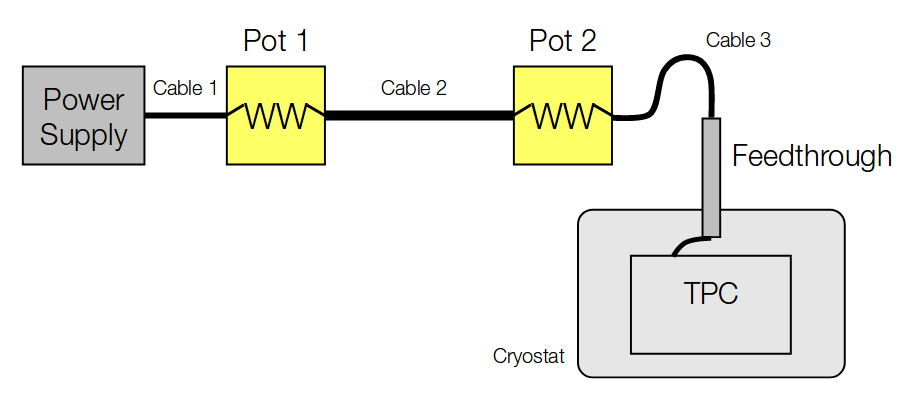
\includegraphics[scale=0.35]{Chapter-3/Images//HVSchematic.png}\\
\caption{Schematic of the LArIAT high voltage system.}
\label{fig:HVScheme}
\end{figure}%See DocDB 1472



The field cage is made of twenty-three parallel copper rings framing the inner walls of the G10 TPC structure. A network of voltage-dividing resistors connected to the field cage rings steps down the high voltage from the cathode to form a uniform electric field. The electric field over the entire TPC drift volume is  486 V/cm (see \ref{ch:AppendixB}). The  maximum drift length, i.e. the distance between cathode and anode planes, is 47 cm.

\subsubsection{Wire planes}
The wire planes measure the charge deposited in the TPC active volume. The drifting charge induces a current on the wire of the inner planes and it is collected on the collection plane wires.
LArIAT counts three wire planes separated by 4 mm spaces: in order of increasing distance from the cathode, they are the shield, the induction and the collection plane. The ``wire pitch", i.e., the distance between two consecutive wires in a given plane, is 4 mm.  The shield plane counts 225 parallel wires of equal length oriented vertically. This plane is not connected with the read-out electronics; rather it shields the outer planes from extremely long induction signals due to the ionization chamber in the whole drift volume. As the shield plane acts almost like a Faraday cage, the shape of signals in the first instrumented plane (induction)  results easier to reconstruct.  Both the induction and collection planes count 240 parallel wires of different length oriented at 60$^\circ$ from the vertical with opposite signs.
Electrons moving past the induction plane will induce a bipolar pulse on its wires and will form a unipolar pulse when collected on the wires of the collection plane. 

The three wire planes and the cathode form three drift volumes, as shown in Figure \ref{fig:driftregions}. 
The main drift volume is defined as the region between the cathode plane and the shield plane (C-S). The other two drift regions are those between the shield plane and the induction plane (S-I), and between the induction plane and the collection plane (I-C). The electric field in these regions is chosen to satisfy the charge transparency condition and allow for 100$\%$ transmission of the drifting electrons through the shield and the induction planes. 

\begin{figure}[htb]
\centering
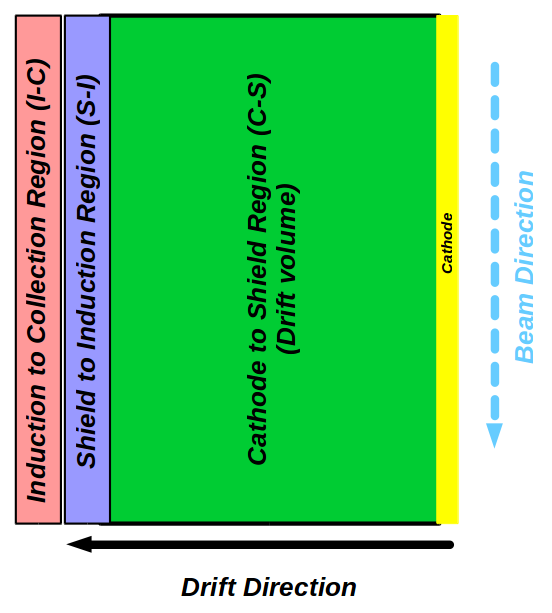
\includegraphics[scale=0.35]{Chapter-3/Images/DriftRegions.png}\\
\caption{Schematic of the three drift regions inside the LArIAT TPC: the main drift volume between the cathode and the shield plane (C-S) in green, the region between the shield plane and the induction plane (S-I) in purple, and the region between the induction plane and the collection plane (I-C) in pink.}
\label{fig:driftregions}
\end{figure}

Table \ref{tab:voltages} provides the default voltages applied to the cathode and the shield, induction, and collection plane.  

\begin{table}[htpb]
\centering
\caption{Cathode and anode planes default voltages}
\label{tab:voltages}
\begin{tabular}{llll}
\hline
\multicolumn{1}{|l|}{ Cathode} & 
\multicolumn{1}{|l|}{ Shield} & \multicolumn{1}{l|}{ Induction} & \multicolumn{1}{l|}{ Collection}  \\ \hline
\multicolumn{1}{|l|}{-23.17 kV} &
\multicolumn{1}{|l|}{-298.8 V} & \multicolumn{1}{l|}{-18.5 V}      & \multicolumn{1}{l|}{338.5 V} \\ \hline
\end{tabular}
\end{table}


\subsubsection{Electronics}

Dedicated electronics read the induction and collection plane wires, for a total of  480-channel analog signal path from the TPC wires to the signal digitizers. A digital control system for the TPC-mounted electronics, a power supply, and a distribution system complete the front-end system. Figure \ref{pic:FEelectronics} shows a block diagram of the overall system. The direct readout of the ionization electrons in liquid argon forms typically small signals on the wires, which needs to be amplified in oder to be processed. LArIAT  performs the amplification stage directly in cold with  amplifiers developed by Brookhaven National Lab (BNL) and mounted on the TPC frame inside the liquid argon, achieving a remarkable Signal-to-Noise ratio. %The BNL ASICs adopted in LAriAT are designated as LArASIC, version 4-star.%The ASIC signals for each wire are then driven out of the vessel  to DAQ boards that act as waveform recorders.
The signal from the ASICs are driven to the other end of the readout chain, to the CAEN V1740 digitizers. The CAEN V1740 has a 12 bit resolution and a maximum input range of 2~VDC, resulting in about 180 ADC count for a crossing MIP.   

\begin{figure}[htbp]
 \centering
 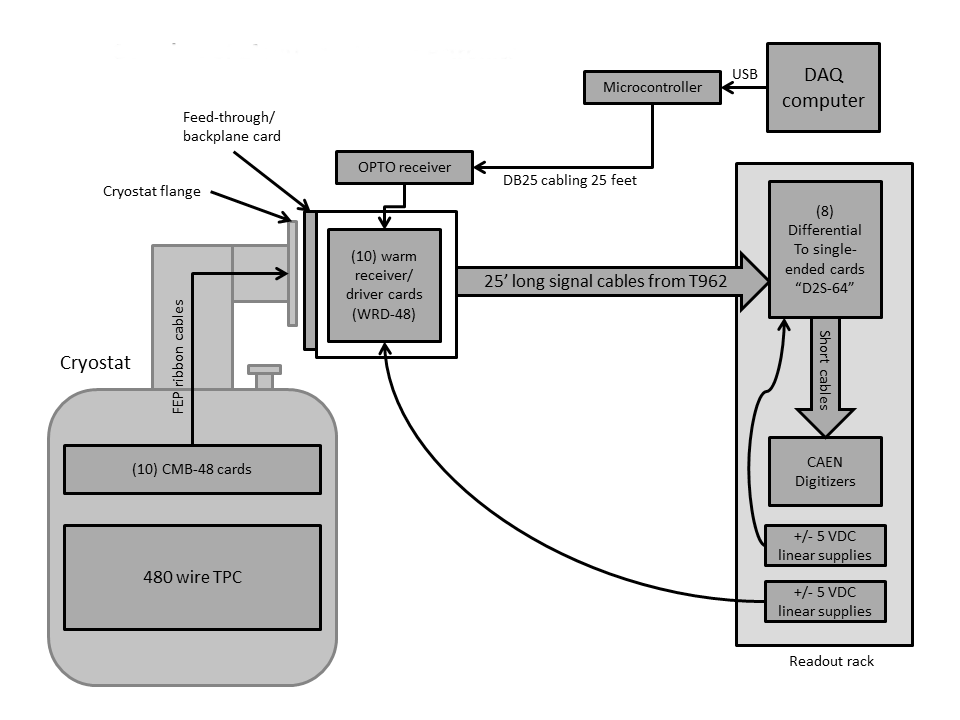
\includegraphics[width=1.0\textwidth]{Chapter-3/Images/LArIAT_FE_Electronics.png}
\caption{Overview of LArIAT Front End electronics. } 
\label{pic:FEelectronics}
\end{figure}




\subsection{LArTPC: Light Collection System}\label{sec:TPCLight}
The mechanism of particle detection in argon other than drift electrons is the collection of scintillation photons.  Over the course of LArIAT three years of data taking, the light collection system changed several times. We describe here the light collection system for Run II. Two PMTs, a 3-inch diameter Hamamatsu R-11065 and 2-inch diameter ETL D757KFL~\cite{lightsys-pmttests}, as well as three SiPMs arrays (two Hamamatsu S11828-3344M 4x4 arrays and one single-channel SensL MicroFB-60035 ) are mounted on the PEEK support structure. PEEK screws into an access flange as shown in Figure~\ref{lightsys_pmts}, on the anode side, leaving  approximately 5~cm of clearance from the collection plane.  

%------------------------------------------
\begin{figure}
\centering
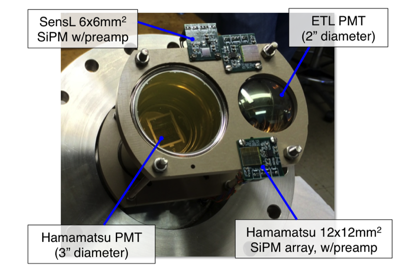
\includegraphics[height=2.2in]{Chapter-3/Images/lightsys_pmts.png}
\hspace{1cm}
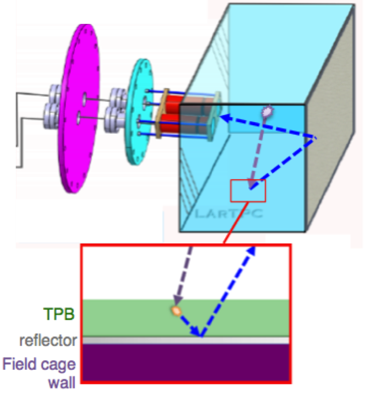
\includegraphics[height=2.2in]{Chapter-3/Images/lightsys_wls.png}
\caption{LArIAT's photodetector system for observing LAr scintillation light inside the TPC (left), and a simplified schematic of VUV light being wavelength-shifting along the TPB-coated reflecting foils (right).}
\label{lightsys_pmts}
\end{figure}
\begin{figure}
\centering
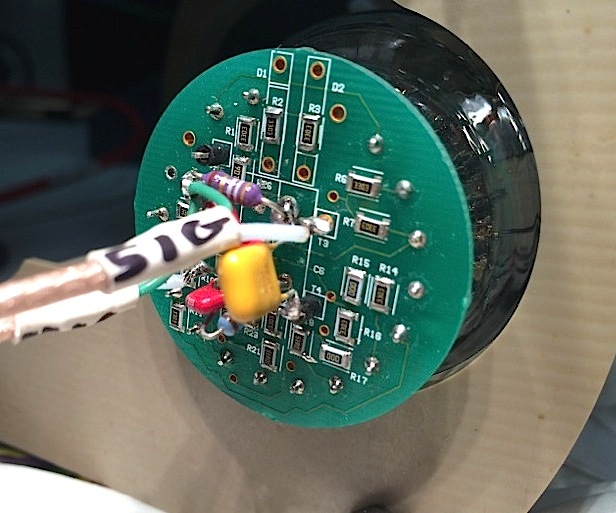
\includegraphics[height=0.25\textheight]{Chapter-3/Images/lightsys_etlbase.jpeg}
\hspace{0.5cm}
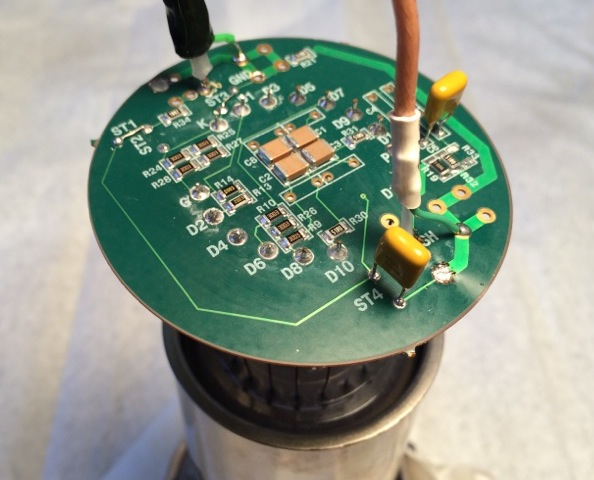
\includegraphics[height=0.25\textheight]{Chapter-3/Images/lightsys_hmmbase.jpg}
\caption{\label{voltagedividers}Photos of the voltage divider bases for the ETL PMT (left) and the Hamamatsu PMT (right) used in Run-II.  The cable connections to the bases seen here were used for powering and testing prior to installation.  The yellow through-hole signal coupling capacitors seen on both bases are 18~nF (X7R) and are rated to 2~kV.}
\end{figure}
%------------------------------------------
Liquid argon scintillates in vacuum-ultraviolet (VUV) range at 128 nm; since cryogenic PMTs are not sensitive to VUV wavelengths, we need to shift the light in a region visible to the PMTs. In LArIAT, the wavelength shifting is achieved by installing on the four walls of the TPC highly-reflective VIKUITY dielectric substrate foils coated with a thin layer of tetraphenyl-butadiene (TPB) (see Figure ~\ref{lightsys_foils}). One or more visible photons  are emitted and reflected into the chamber during the interaction of a VUV photon interacts with the TPB. Thus, the light yield is increased and made more uniform across the TPC active volume, allowing the possibility of light-based calorimetry (under study).

%------------------------------------------
%\begin{figure}
%\centering
%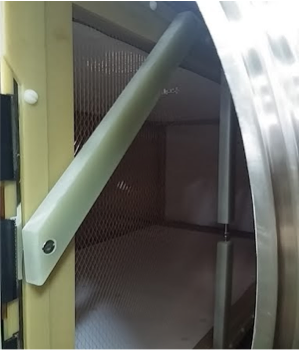
\includegraphics[scale=1.3]{Chapter-3/Images/lightsys_foils.png}
%\caption{\label{lightsys_foils}The TPB-coated reflector foils mounted to the TPC field cage walls as viewed through the front cryostat opening. {\textcolor{red}{Better pictures needed.}}}
%\end{figure}
%------------------------------------------

For Run II, we coated both  the windows of the ETL PMT and SensL SiPM  with a thin layer of TPB. In doing so, some of the VUV scintillation light converts into visible right at the sensor faces, keeping information on the direction of the light source. Information about the light directionality is lost for light reflected on foils, as the reflection is uniform in angle. For Run-II, the voltage dividers for the PMTs were configured for positive bias with a DC-coupled anode (AC-coupled anode with grounded photocathode) to minimize induced noise on the TPC wires and modify the PMT bases accordingly.  



\section{Trigger and DAQ}
The LArIAT DAQ and trigger system governs the read out of all the many subsystems forming LArIAT. 
The CAEN V1495 module and its user-programmable FPGA  are the core of this system.  Every 10~ns, this module checks for matches between sixteen logical inputs and user-defined patterns in the trigger menu; if it finds a match for two consecutive clock ticks, that trigger fires.

The beam instruments,  the cosmic ray taggers, and the light collection system provide NIM-standard logic pulse inputs to the trigger decision. We automatically log the trigger inputs configuration with the rest of the DAQ configuration at the beginning of each run.

Fundamental inputs to the trigger card come from the TOF (see Sec.~\ref{sec:TOF}) and the wire chambers (see Sec.~\ref{sec:MWPC}), as activity in these systems points to the presence of a charged particle in tertiary beam line.
In particular, the discriminated pulses from the TOF PMTs form a NIM logic pulse for the trigger logic. We ask for a coincidence within a 20~ns window for all the pulses from the PMTs looking at the same scintillator block and use the coincidence int the upstream and downstream paddle to inform the trigger decision. In order to form a coincidence between the upstream and downstream paddles, we delay the upstream paddle coincidence by 20~ns and widen it by 100~ns. The delay and widening are necessary to account for both  lightspeed particles and slower particles (high-mass) to travel the 6.5~m between the upstream and the downstream paddles. 
Four multi-hit TDCs read out each wire chamber: two TDC per plane (horizontal and vertical), sixty-four wires per TDC. In each TDC, we keep the logical ``OR" for any signal over threshold from the sixty-four wires. We then require a coincidence between the ``OR" for the horizontal TDCs and the ``OR" for the vertical TDCs: with this logic we make sure that at least one horizontal wire and one vertical wire saw significant signal in one wire chamber.  The single logical pulse from each of the four wire chambers feeds into the first four inputs to the V1495 trigger card. We require a coincidence within 20~ns of at least three logical inputs to form a trigger.


%Another primary input to the trigger card is from the cosmic towers (see Section~\ref{sec:CosmicRayPaddle}). To capture cosmic ray events in which a minimally ionizing cosmic ray muon crossed the TPC along the body diagonal, NIM modules form the logical coincidences from the two cosmic towers, one upper and one lower paddle assembly, in each combination.  The OR of these is provided as an input to the V1495. 

%Three important logic pulses are derived from the timing of the beam.  These include a pulse in a brief window before the beam, a pulse indicating that the beam is on, and a pulse which defines the beam-free period which may be used for collecting cosmic-ray events.  An adjustable pulser is a fourth trigger input which does not depend on any particular activity in the experiment hall,  useful for collecting background events with zero bias. 

%%%%%%%%%%%%%%%%%%%%%%

%The PMTs observing liquid argon scintillation light (see Section \ref{sec:PhotonSystem}) produce pulses which form the foundation of several interesting trigger inputs.  Thresholding a copy of each PMT pulse (after amplification), and requiring a coincidence of pulses within $\sim$20~ns, creates simple trigger inputs indicating ionizing radiation was produced in the TPC.  This scintillation logic pulse is used to initiate a gate which spans the length of the TPC drift time, creating a logic signal which is remains ``on'' while significant drift charge may still be present in the TPC.  In addition, requiring a delayed coincidence of two subsequent scintillation logic pulses, separated by a variable length of time ranging from 300~ns to 7~$\mu$s, is used to create a trigger input to select events where a cosmic muon stops and decays to a Michel electron in the TPC.  A few different versions of this light-based trigger were implemented throughout the course of LArIAT's run time to allow reconstruction and calorimetric studies of Michel electrons. Figure~\ref{michel_logic} shows a schematic diagram of the logic comprising the Michel electron trigger. 

%\begin{figure}
%\includegraphics[width=\textwidth]{figures/trigger_michellogic.png}
%\caption{\label{michel_logic}A schematic diagram of the trigger logic used to select Michel electron events during the cosmic readout window of the LArIAT supercycle.  The two PMT signals refer to the Hamamatsu (``HMM'') and ETL PMTs described in Section~\ref{sec:PhotonSystem}.  For some data-taking periods in Run-II, un-amplified pulses were discriminated at 180 mV to act as a veto on events that may saturate the dynamic range of the V1751 digitizer.  The discriminator thresholds used on the amplified (x10) PMT signal copies (\emph{ThA}, \emph{ThB}) as well as the Gate Delay period, were adjusted between run periods while experimenting with different configurations.}
%\end{figure}

%Further trigger inputs come from the beam line instrumentation behind the LArTPC cryostat, the PMTs of the Punch-Through scintillator paddles and those of the scintillator paddles instrumenting the Muon Range Stack.  The PMT pulses of all four of the broad-faced Punch Through paddles are discriminated to form logic pulses.  A single logic pulse is formed from these, indicating activity in at least two overlapping paddles at the rear of cryostat, before the steel block of the range stack.  PMT pulses from the Muon Range Stack are amplified and threshold discriminated.  These MuRS paddle pulses are then combined as in the Punch Through, creating single-bit indicators for each of the four instrumented layers that at least one pair of overlapping scintillator paddles sent signals within a 20~ns coincidence window.

%\subsubsection{Trigger Decision and Issuance}

%The V1495 may be configured to have up to sixteen trigger patterns and sixteen veto patterns, based on the trigger input signals.  A trigger pattern is defined as the AND of one or more defined inputs, and may include the NOT of the AND of further inputs.  Veto patterns are independently defined in the same way, but they have a very different effect.  When any of the trigger patterns fire, a ``fast trigger'' signal is issued and an adjustable countdown is initiated.  If the countdown completes without a veto pattern firing, the ``slow trigger'' signal is also issued and on a distinct hardware channel. Otherwise, if a veto pattern fires during the countdown, the slow trigger signal is vetoed.  

%The fast trigger signal prompts readout of all the `short' data buffers, which include the V1751 modules, the V1495 itself, and the MWPC controller.  The V1751 buffers typically contain digitized PMT signals from the time of flight and cryogenic light collection detectors. Readout of the TPC wire signals, which are much longer and more numerous, is only prompted at the issuance of the slow trigger.



\section{Control Systems}
LArIAT is a complex ensemble of systems which needed to be monitored at once during data taking.  We performed the monitoring of the systems operations with a slow control system, a DAQ monitoring system and a low level data quality monitoring described in the following sections.

\subsubsection{Slow Control}
We used the Synoptic Java Web Start framework as a real-time display of subsystem conditions. Its simple 
Graphical User Interface allowed us to change the operating parameters and to graph the trends of several variables of interest for all the tertiary beam detectors.  Among the most important quantities monitored by Synoptic there are the level of argon in both the inner vessel and the external dewar, the operating voltages of cathode and wire planes, of the PMTs and SiPMs, and of the four wire chambers, as well as the magnets temperature. Figure \ref{fig:synoptics} shows an example of the monitoring system.
LArIAT uses the Accelerator Control NETwork system (ACNET) to monitor the beam conditions of the MCenter beamline. For example, the X and Y position of the beam at the first two wire chambers (WC1 and WC2) are shown in \ref{fig:ACNET}. 

\begin{figure}[htb]
\centering
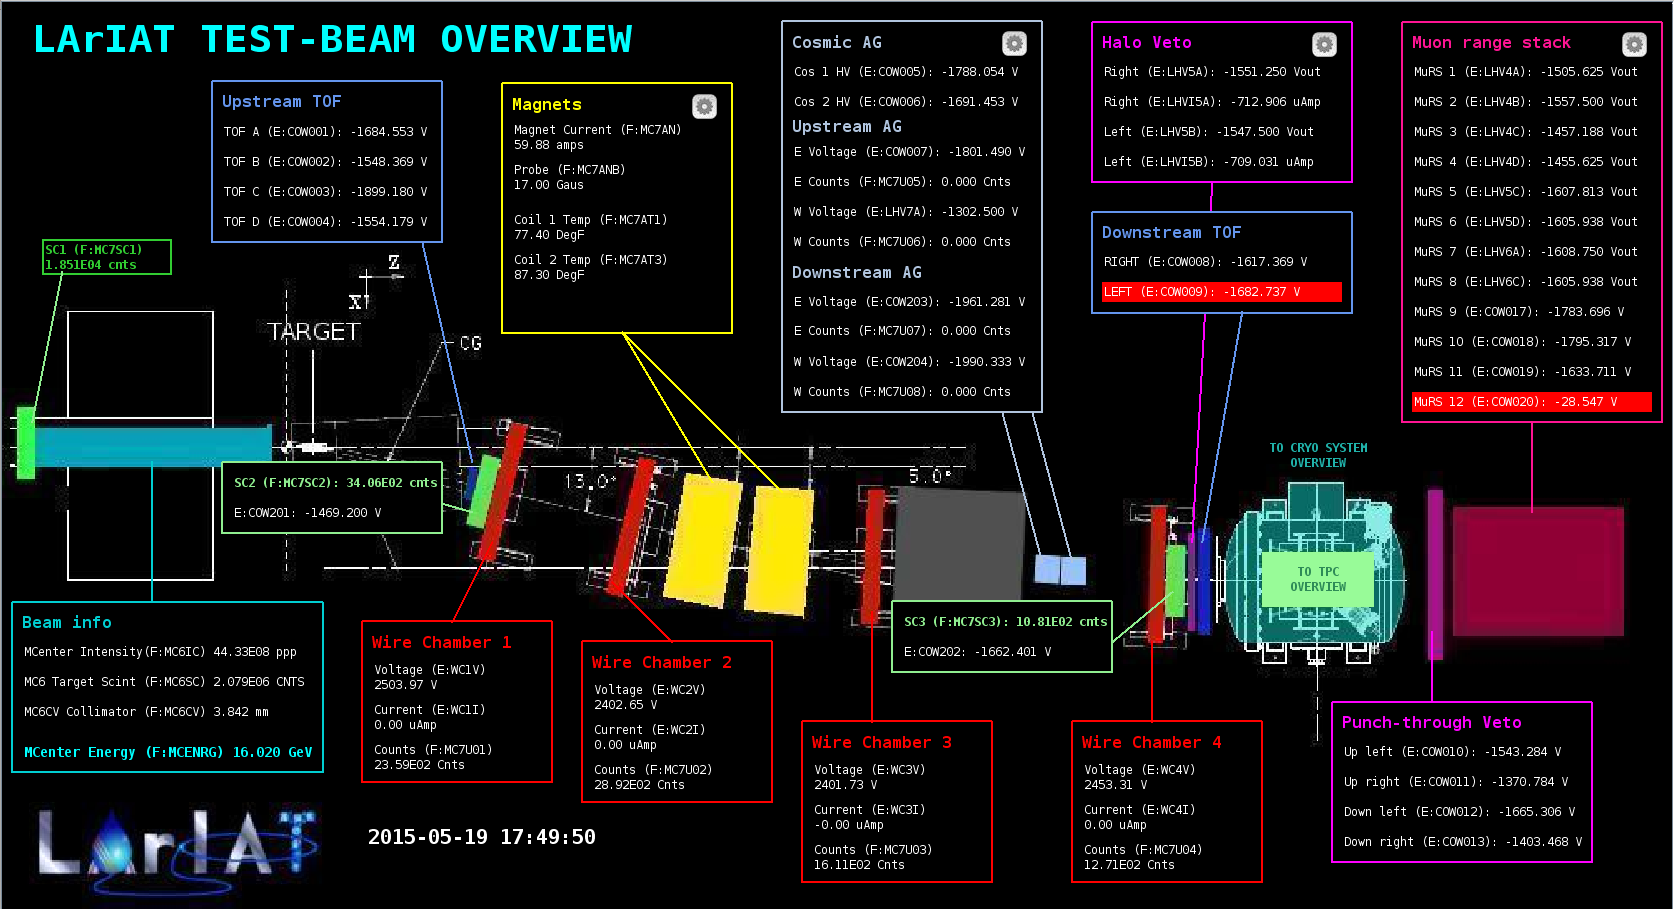
\includegraphics[width=\textwidth,height=\textheight,keepaspectratio]{Chapter-3/Images/BeamOverview.png}
\caption{Interface of the Synoptic slow control system}
\label{fig:synoptics}
\end{figure}

\begin{figure}[htb]
\centering
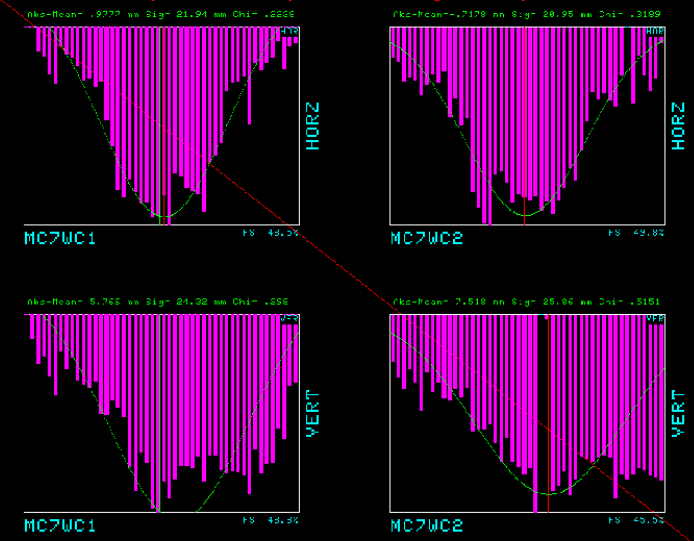
\includegraphics[scale=0.5]{Chapter-3/Images/BeamPosition.png}
\caption{Beam position at the upstream wire chambers monitored with ACNET.}
\label{fig:ACNET}
\end{figure}

\subsubsection{DAQ Monitoring}

We monitor the data taking and the run time evolution with the Run Status Webpage (\href{http://lariat-wbm.fnal.gov/lariat/run.html}{http://lariat-wbm.fnal.gov/lariat/run.html}), a  webpage updated in real-time.  The page displays, among other information, the total number of triggers in the event per CAEN digitizer board, the total number of detectors triggered during a beam spill,  the trigger patterns (the number of times a particular trigger pattern was satisfied  during a beam spill) and current time relative to the Fermilab accelerator complex supercycle. A screen shot of the page is show in figure \ref{fig:runcond}.

\begin{figure}[htb]
\centering
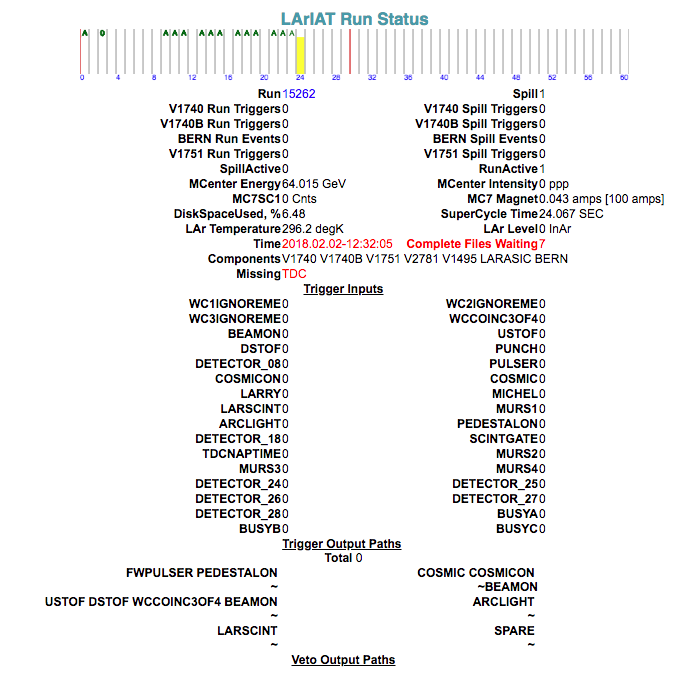
\includegraphics[scale=0.6]{Chapter-3/Images/RunConditions.png}
\caption{Run Status page at LArIAT downtime. At the top the yellow bar displays the current position in the Fermilab supercycle. Interesting information to be monitored by the shifter were the run number and number of spills, time elapsed from data taking (here in red), the energy of the secondary beam and the trigger paths.}
\label{fig:runcond}
\end{figure}



\subsubsection{Data Quality Monitoring}
We employ two systems to ensure the quality of out data during data taking: the Near-real-time Data Quality Monitoring and the Event Viewer.

\href{http://lariat-daq01.fnal.gov:5000/}{The Near-real-time Data Quality Monitoring} (DQM). This webpage receives updates from all the VME boards in the trigger system and displays the results of a quick analysis of the DAQ stream of raw data on a spill-by-spill basis. The DQM allows the shifter to monitor almost in real time (typically with a 2-minute delay)  a series of low level-quantities and compare them to past collections of beam spills. Some of the variables monitored in the DQM are  the pedestal mean and RMS on CAEN digitizer boards
of the TPC wires and PMTs of the beamline detectors, the hit occupancy and timing plots on the multi-wire chambers, and number of data fragments recorded that are used to build a TPC event. Abnormal values for  low-level quantity in the data  activate a series of alarms in the DQM; this quick feedback on the DAQ and beam conditions is fundamental to assure a fast debugging of the detector and a very efficient data taking during beam uptime.

The online Event Viewer displays a two dimensional representation of LArIAT TPC events on both the Induction and the Collection planes in near real time. The raw pulses collected by the DAQ on each wire are plotted as a function of drift time, resulting in an image of the TPC event easily readable by the shifter. This tool guarantees a particularly good  check of the TPC operation which activate an immediate feedback for troubleshooting a number of issues. For example,  it easy for the shifter to spot high occupancy events and request a reduction of the primary beam intensity, or to spot a decrease of the argon purity which requires the regeneration of filters, or to catch the presence of electronic noise and reboot the ASICs. An example of high occupancy event is shown in \ref{fig:highOcc}.

\begin{figure}[htb]
\centering
%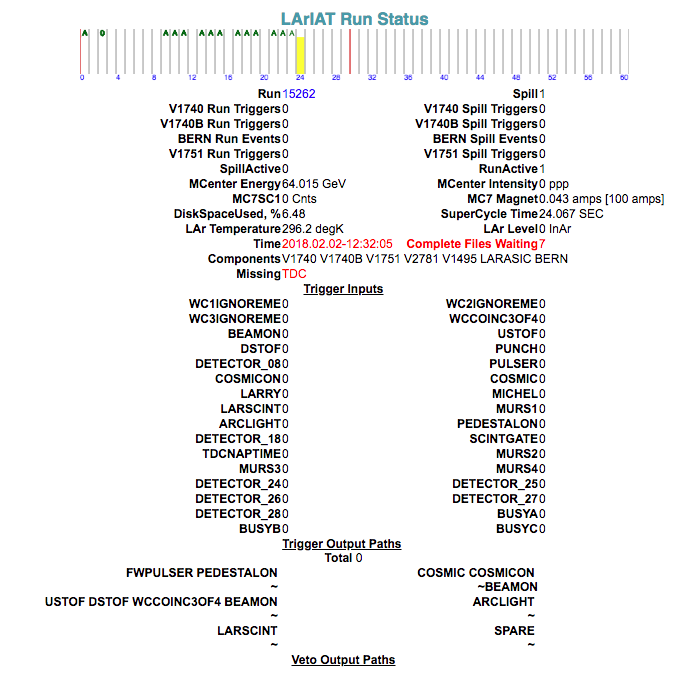
\includegraphics[scale=0.6]{Chapter-3/Images/RunConditions.png}
\caption{High occupancy event display.}
\label{fig:highOcc}
\end{figure}



\chapter{Total Hadronic Cross Section Measurement Methodology}\label{ch:Interactions}
{\raggedleft ``\emph{Like a lemon to the lime and the bubble to the bee}" \par}
{\raggedleft -- Eazy-E,   1993 -- \par}%Gimmie that *,
\vspace{0.5cm}

This chapter describes the general procedure employed to measure  total hadronic interaction cross sections on Ar in LArIAT.
Albeit with small differences, both the  ($\pi^{-}$,Ar) and (K$^{+}$,Ar) total hadronic cross section measurements rely on the same procedure. We start by selecting the particle of interest using a combination of beamline detectors and TPC information (Section \ref{ch:ParticleSelectionMethod}). We then perform a handshake between the beamline information and the TPC tracking to assure the selection of the correct TPC track (Section \ref{ch:WC2TPCMatchMethod}) associated to the corresponding beam particle. We then apply the ``thin slice" method to measure the ``raw" hadronic cross section (Section \ref{ch:ThinSliceMethod}). A series of corrections are then evaluated and applied to obtain the final cross section (Section \ref{ch:MCCorrections}). 

At the end of this chapter, we show a sanity check of the methodology by applying the thin slice method employing only MC truth information and retrieving the expected MC cross section for pions and kaons (Section \ref{ch:procedureTesting}).



\section{Event Selection}\label{ch:ParticleSelectionMethod}
The measurement of the ($\pi^{-}$,Ar) and (K$^{+}$,Ar) total hadronic cross section in LArIAT starts by selecting the pool of pion or kaon candidates and measuring their momentum before they enter the LAr volume.  This is done through the series of selections on  beamline and TPC information described in the next sections. The summary of the event selection in data is reported in Table \ref{tab:beamlineDataSelection}.


\begin{table}[b]
\centering
\begin{tabular}{|l|c|c|}
\hline
                                                        & Run-II Neg Pol   &  Run-II Pos Pol  \\ \hline
1. Events Reconstructed in Beamline        &  158396  & 260810  \\ \hline
2. Events with Plausible Trajectory            &   147468 & 240954  \\ \hline
3. Beamline $\pi^-/\mu^-/e^-$  Candidate  &   138481 &     N.A.   \\ \hline
4. Beamline $K^+$   Candidate                 &    N.A       & 2837     \\ \hline
5. Events Surviving Pile Up Filter              &   108929  & 2389       \\ \hline
6. Events with WC2TPC Match                 &    41757   & 1081 \\ \hline
7. Events Surviving Shower Filter             &    40841    &  N.A.     \\ \hline
8. Available Events For Cross Section      &   40841    &   1081    \\ \hline
\end{tabular}
\caption{Number of data events for Run-II Negative and Positive polarity }
\label{tab:beamlineDataSelection}
\end{table}


\subsection{Selection of Beamline Events}\label{ch:beamlineDetectorsData}
We leverage the beamline particle identification and momentum measurement before entering the TPC as an input to evaluate the kinetic energy for the hadrons used in the  cross sections measurements. To this end, we select the LArIAT data to keep only events whose wire chamber and time of flight information is registered (line 1 in in Table \ref{tab:beamlineDataSelection}). Additionally, we perform a check of the plausibility of the trajectory inside the beamline detectors: given the position of the hits in the four wire chambers, we make sure the particle's trajectory does not cross any impenetrable material such as the collimator and the magnets steel (line 2 in in Table \ref{tab:beamlineDataSelection}).


\subsection{Particle Identification in the Beamline}
In data, the main tool to establish the identity of the hadron of interest is the LArIAT tertiary beamline, in its function of mass spectrometer. We combine the measurement of the time of flight, $TOF$, and the beamline momentum, $p_{Beam}$, to reconstruct the invariant mass of the particles in the beamline, $m_{Beam}$, as follows
\begin{equation}
m_{Beam} = \frac{p_{Beam}}{c}\sqrt{\biggl(\frac{TOF*c}{l}\biggr)^2 -1},
\label{eq:mass}
\end{equation}
 where $c$ is the speed of light and $l$ is the length of the particle's trajectory between the time of flight paddels. 

Figure \ref{fig:mass} shows the mass distribution for the Run II negative polarity runs on the left and positive polarity runs on the right. We perform the classification of events into the different samples as follows:

\begin{itemize}
\item \underline{$\pi/\mu/e$:}  mass $<$ 350~MeV/c$^2$

\item \underline{kaon:} 350~MeV $<$ mass $<$ 650~MeV/c$^2$

\item \underline{proton:} 650~MeV $<$ mass $<$ 3000~MeV/c$^2$.

\end{itemize}

Lines 3 and 4 in in Table \ref{tab:beamlineDataSelection} show the number of negative $\pi/\mu/e$ and positive $K$ candidates which pass the mass selection for LArIAT Run-II data.

%\begin{comment}     
\begin{figure}
  \centering  
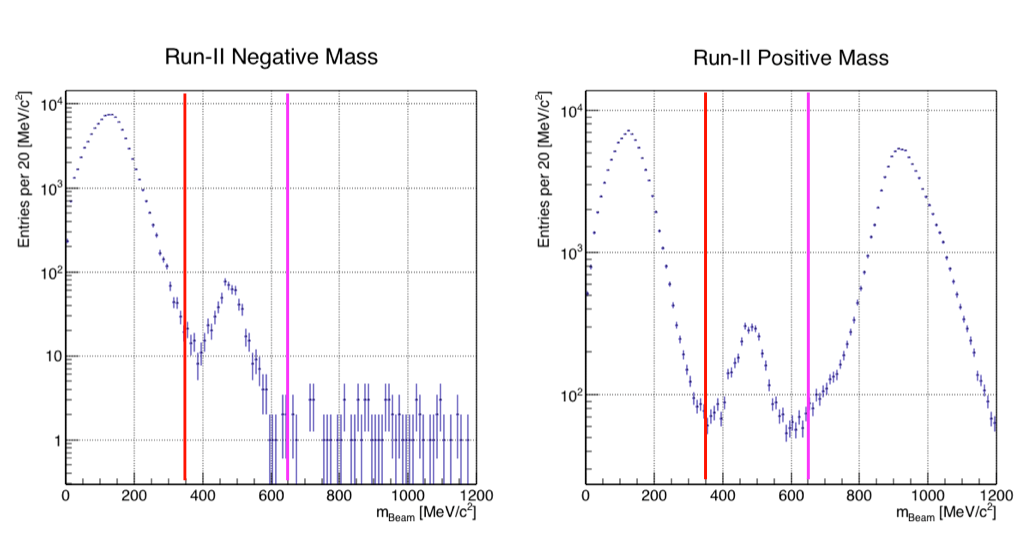
\includegraphics[width=\textwidth]{Chapter-4/Images/massRunII.png}
\caption{Distribution of the beamline mass as calculated according to equation \ref{eq:mass} for the Run-II events reconstructed in the beamline, negative polarity runs on the left and positive polarity runs on the right. The classification of the events into $\pi^\pm/ \mu^\pm/e^\pm$, K$^\pm$, or (anti)proton is based on these distributions, whose selection cut are represented by the vertical colored lines.}
\label{fig:mass}
\end{figure}

\subsection{TPC Selection: Halo Mitigation }\label{ch:pileUp}
The secondary beam impinging on LArIAT secondary target produces a plethora of particles which propagates downstream. The presence of upstream and downstream collimators greatly abates the number of particles tracing down the LArIAT tertiary beamline. However, it is possible that more than one particle sneaks into the LArTPC during its readout time: the TPC readout is triggered by the particle  firing the series of beamline detectors along our tertiary beamline, but particles from the beam halo might also be present in the TPC at the same time. We call ``pile up" the additional traces in the TPC. We adjusted the primary beam intensity between LArIAT Run I and Run II to reduce the presence of events with high pile up particles in the data sample. For the cross section analyses, we remove events with more than 4 tracks in the first 14 cm upstream portion of the TPC from the sample (line 5 in in Table \ref{tab:beamlineDataSelection}).


\subsection{TPC Selection: Shower Removal}\label{ch:electrons}
In the case of the ($\pi^-$,Ar) cross section, the resolution of  beamline mass spectrometer is not sufficient to select a beam of pure pions. In fact,  muons which are close in mass to the pions and relativistic electrons survive the selection on the beamline mass.  It is important to notice that the composition of the negative polarity beam is mostly pions, as will be discussed in section \ref{ch:beamlineComposition}.
Still, we devise a selection on the TPC information to mitigate the presence of electrons in the sample used for the pion cross section. The selection relies on the different topologies of a pion and an electron event when propagating in liquid argon: while the former will trace a track inside the TPC active volume, the latter will tend to ``shower", i.e. interact with the medium, producing bremsstrahlung photons which pair convert into several short tracks. In order to remove the shower topology, we create a region of interest (ROI) around the TPC track corresponding to the beamline particle. We look for short tracks contained in the ROI, as depicted in figure \ref{fig:showerFilt}:  if more then 5 tracks shorter than 10 cm are in the ROI, we reject the event. Line 7 in in Table \ref{tab:beamlineDataSelection} shows the number of events surviving this selection.

\begin{figure}
  \centering  
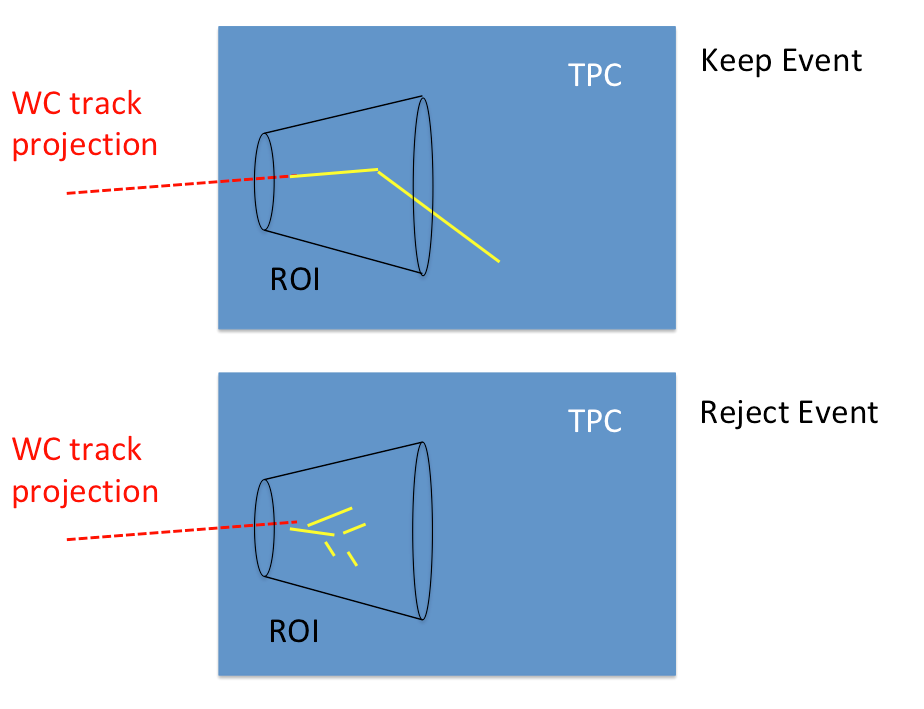
\includegraphics[width=\textwidth]{Chapter-4/Images/Shower.png}
\caption{Visual rendering of the shower filter. The ROI is a cut cone, with a small radius of 4 cm, a big radius of 10 cm and an height of 42 cm (corresponding to 3 radiation lengths for electrons in Argon).}
\label{fig:showerFilt}
\end{figure}



\section{Beamline and TPC Handshake: the Wire Chamber to TPC Match}\label{ch:WC2TPCMatchMethod}
For each event passing the selection on its beamline information, we need to identify the track inside the TPC corresponding to the particle which triggered the beamline detectors, a procedure we refer to as ``WC to TPC match" (WC2TPC for short). In general, the TPC tracking algorithm can reconstruct more than one track in the event, partially due to the fact that hadrons interact in the chamber and partially because of pile up particles during the triggered TPC readout time, as shown in figure~\ref{fig:kaonInteraction}. 


\begin{figure}
  \centering  
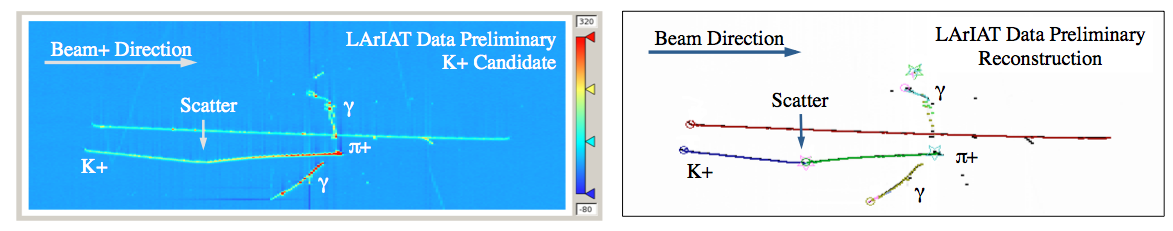
\includegraphics[width=\textwidth]{Chapter-4/Images/KaonExample.png}
\caption{Kaon candidate event: on the right, event display showing raw quantities; on the left, event display showing reconstructed tracks. In the reconstructed event display, different colors represent different track objects. A kink is visible in the kaon ionization, signature of a hadronic interaction: the tracking correctly stops at the kink position and two tracks are formed. An additional pile-up track is so present in the event (top track in red).}
\label{fig:kaonInteraction}
\end{figure}



We attempt to uniquely match one wire chamber track (see Section \ref{sec:MWPCfunc}) to one and only one reconstructed TPC track. 
In order to determine if a match is present, we apply a geometrical selection on the relative position of the wire chamber and TPC tracks. 
We start by considering only TPC tracks whose first point is in the first 2 cm upstream portion of the TPC for the match.  We project the wire chamber track to the TPC front face where we define the coordinates of the projected point as  $x_{FF}$ and $y_{FF}$.  For each considered TPC track, we define $\Delta$X as the difference between the $x$ position of the most upstream point of the TPC track and $x_{FF}$.  $\Delta$Y is defined analogously. We define the radius difference, $\Delta$R, as $ \Delta \text{R} =  \sqrt{ \Delta \text{X}^2 +  \Delta \text{Y}^2}  $. We define  as $\alpha$ the angle between the incident WC track and the TPC track in the plane that contains them.  If  $\Delta \text{R} < 4 $~cm, $\alpha < 8^\circ $,  a match between WC-track and TPC track is found. We describe  how we determine the value for the radius and angular selection in Section \ref{ch:WC2TPCMatchOptimization}.
We discard events with multiple WC2TPC matches. We use only those TPC tracks that are matched to WC tracks in the cross section calculation. Line 6 in Table \ref{tab:beamlineDataSelection} shows the number of events where a unique WC2TPC match was found.

In MC, we mimic the matching between the WC and the TPC track by constructing an artificial WC track using truth information at wire chamber four. We then apply the same WC to TPC matching algorithm as in data. 


\begin{figure}
  \centering  
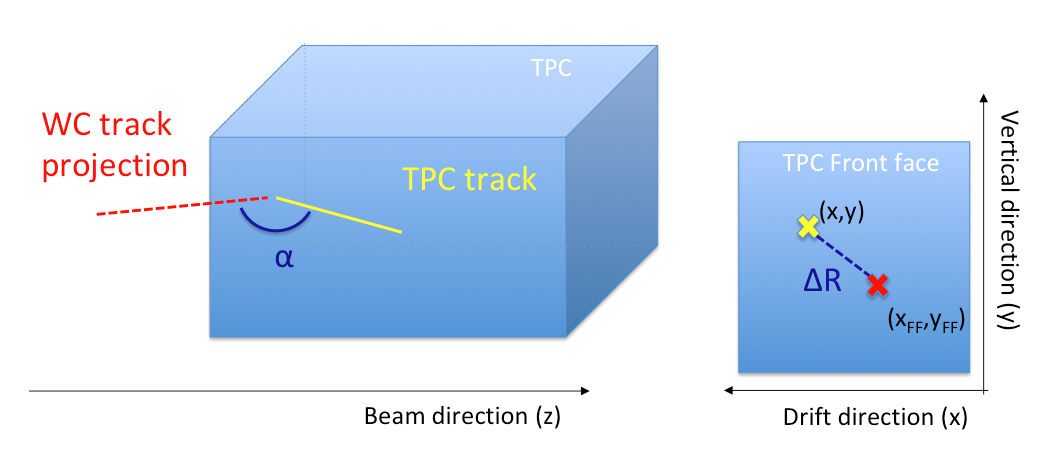
\includegraphics[width=\textwidth]{Chapter-4/Images/WC2TPCMatchTracks.png}
\caption{Visual rendering of the wire chamber to TPC match.}
\label{fig:showerFilt}
\end{figure}

\section{The Thin Slice Method}\label{ch:ThinSliceMethod}



Once we have selected the 40841 beamline pion candidates  and the 1081 beamline kaon candidates, and we have identified the TPC corresponding track, we apply the thin slice method to measure the cross section, as the following sections describe. 
\subsection{Cross Sections on Thin Target}
Cross section measurements on a thin target have been the bread and butter of nuclear and particle experimentalists since the Geiger-Marsden experiments \cite{Geiger1909}. At their core, this type of experiments consists in shooting a beam of particles with a known flux on a thin slab of material and recording the outgoing flux. 


In general even in the case of thin target, the target is not a single particle, but rather a slab of material containing many diffusion centers. The so-called  ``thin target" approximation assumes that the target centers are uniformly distributed in the material and that the target is thin compared to the projectile interaction length, so that no center of interaction sits in front of another. In this approximation, the ratio between the number of particles interacting in the target $N_{\text{Int}}$ and the number of incident particles $N_{\text{Inc}}$ on the target estimates the interaction probability $P_{Interacting}$, which is the complementary to one of the survival probability $P_{Survival}$. 
Equation \ref{eq:thinTargetXS} 
\begin{equation}
P_{Survival} = 1- P_{Interacting} = 1 - \frac{N_{\text{Int}}}{N_{\text{Inc}}} = e^{-\sigma_{TOT}\text{ } n \text{ }\delta X}
\label{eq:thinTargetXS}
\end{equation}
describes the probability for a particle to survive the thin target. This formula relates  the interaction probability to the total hadronic cross section ($\sigma_{TOT}$), the density of the target centers ($n$)\footnote{The scattering center density in the target, {\emph{n}},  relates to the argon density $\rho$, the Avogadro number  $ N_{A} $ and the argon molar mass $m_A$ as $n=\frac{\rho N_{A} }{m_A}$.}    and  the thickness of the target  along the incident hadron direction ($\delta X$). If the target is thin compared to the interaction length of the process considered, we can Taylor expand the exponential function in equation \ref{eq:thinTargetXS} and find a simple proportionality relationship between the cross section and the number of incident and interacting particles, as shown in equation \ref{eq:thinTargetXSTaylor}:
\begin{equation}
1 - \frac{N_{\text{Int}}}{N_{\text{Inc}}} =  1 -\sigma_{TOT} \text{  }n \text{  }\delta X + O(\delta X^2).
\label{eq:thinTargetXSTaylor}
\end{equation}

Solving for the cross section, we find:
\begin{equation}
 \sigma_{TOT}  = \frac{1}{n \text{ }\delta X}\frac{N_{\text{Int}}}{N_{\text{Inc}}}.
\label{eq:thinTargetXSSolved}
\end{equation}

\subsection{Not-so-Thin Target: Slicing the Liquid Argon Volume}\label{ch:XSRaw}
The interaction length of pions and kaons in liquid argon is expected to be of the order of 50 cm for pions and 100 cm for kaons. Thus, the LArIAT TPC, with its 90 cm of length, is not a thin target. However, the fine-grained tracking of the LArIAT LArTPC allows us to treat the argon volume as a sequence of many adjacent thin targets. 

As described in Chapter \ref{sec:experimentDescription}, LArIAT induction and collection planes consist of 240 wires each at 4 mm spacing. The wires are oriented at +/- $60^{\circ}$ from the vertical direction, while the beam direction is oriented 3 degrees off the $z$ axis in the $XZ$ plane.  The collection wires collect signals proportional to the energy deposited by the hadron along its path in a  $\delta${\emph{X}} = 4 mm/(sin($60^{\circ}$)cos($3^{\circ}$)) $\approx$ 4.7~mm slab of liquid argon. Thus, one can think to slice the TPC into many thin targets of $\delta${\emph{X}} = 4.7~mm thickness along the direction of the incident particle, making a measurement at each wire along the path.

Considering each slice {\emph{j}}  a ``thin target",  we can apply the cross section calculation from Equation~\ref{eq:thinTargetXSSolved} iteratively, evaluating the kinetic energy of the hadron as it enters each slice, $E_{j}^{kin}$.  For each WC2TPC matched particle, the energy of the hadron entering the TPC is known thanks to the momentum and mass determination by the tertiary beamline, 

\begin{equation}
 E^{kin}_{Front Face}  = \sqrt{p^2_{Beam} - m^2_{Beam}} - m_{Beam} - E_{loss},
\label{eq:enFF}
\end{equation}
where $E_{loss}$ is a correction for the kinetic energy loss in the uninstrumented material between the beamline and the TPC front face. While propagating through the target,  the kinetic energy of the hadron at each slab is determined by subtracting the energy deposited by the particle in the previous slabs. For example, at the $j^{th}$ slab of a track, the kinetic energy will be

\begin{equation}
 E_{j}^{kin} =  E^{kin}_{Front Face} - \sum_{i < j} E_{\text{Dep},i},
\label{eq:KEj}
\end{equation}
where $E_{\text{Dep},i}$ is the energy deposited at each argon slice before the $j^{th}$ point as measured by the calorimetry associated with the tracking.


If the particle enters a slice, it contributes to the $N_{\text{Inc}}( E^{kin})$ distribution in the energy bin corresponding to its kinetic energy in that slice. While into the slice, a hadron may or may not interact. If it interacts in the slice, it  contributes also to the $N_{\text{Int}}(E^{kin})$ distribution in the appropriate energy bin; this occurrence corresponds to the end of the hadron tracking. If the hadron does not interact, it will enter the next slice and the interaction evaluation starts again.
The process is applied to all the hadrons in the sample; the cross section as a function of kinetic energy, $\sigma_{TOT}( E^{kin})$ is then evaluated to be proportional to the ratio $\frac{N_{\text{Int}}( E^{kin})}{N_{\text{Inc}}( E^{kin})}$ -- bin by bin ratio. 


Our goal is to measure the total interaction cross section, independently  from the topology of the interaction. Thus, we determine that a hadron interacted simply by requiring that the last point of the WC2TPC matched track lies in a slice within the fiducial volume, whose boundaries are defined in Table \ref{tab:FidVol}. If the TPC track ends within the fiducial volume, its last point will be the interaction point; if the track crosses the boundaries of the fiducial volume, the track will be considered ``through going" and no interaction point will be found. The only points of the hadronic candidate track considered to fill the  $N_{\text{Int}}$ and  $N_{\text{Inc}}$ distributions are the ones contained in the fiducial volume. 
 
 A notable background pertinent only to the $N_{\text{Int}}$  distribution are cases in which the hadrons decays inside the TPC. In those cases in fact, the tracking ends inside the TPC but the interaction is not hadronic. The handling of decay background is treated in a slightly different way for the pion and kaon section, details can be found in sections \ref{ch:PionXSBkgSub} and \ref{ch:KaonXSRaw} respectively.



\begin{table}[t]
\centering
\begin{tabular}{|l|r|r|}
\hline
& min   &  max  \\ \hline
$X$ & 1 cm   & 46 cm  \\ \hline
$Y$ & -15 cm   & 15  cm  \\ \hline
$Z$ & 0 cm   & 86 cm  \\ \hline
\end{tabular}
\caption{Fiducial volume boundaries used to determine cross section interaction point. }
\label{tab:FidVol}
\end{table}



\subsection{Corrections to the Raw Cross Section}\label{ch:MCCorrections}
%%%%%%%%%%%%%%%%%%%%%%%%%%
Equation \ref{eq:thinTargetXSSolved}  is a prescription for measuring the cross section in case of a pure beam of the hadron of interest and 100\% efficiency in the determination of the interaction point.  For example, if LArIAT had a beam of pure pions and were 100\% efficient in determining the interaction point within the TPC, the pion cross section as a function of  kinetic energy (estimated at the central value of the energy bin $E_i$) would be given by

\begin{equation}
 \sigma^{\pi^-}_{TOT}(E_{i})  = \frac{1}{n \delta X}\frac{N^{\pi^-}_{ \text{Int}} (E_{i})}{N^{\pi^-}_{ \text{Inc}}(E_{i})}.
\label{eq:thinTargetXSSolved2}
\end{equation}

Unfortunately, this is not the case. In fact, the selection used to isolate pions in the LArIAT beam allows for the presence of some muons and electrons as background, while the kaon selection allows for a small contamination of protons (see Section \ref{ch:beamlineComposition}). Also, the LArIAT TPC tracking algorithm is not 100\% efficient in determining the interaction point. Therefore we need to apply two corrections evaluated on the MC in order to extract the final cross section from LArIAT data: i) a background subtraction and ii) a correction for reconstruction effects. 
Still using the pion case as example, we estimate the pion cross section in each energy bin changing  Equation \ref{eq:thinTargetXSSolved2} into
\begin{equation}
 \sigma^{\pi^-}_{TOT}(E_{i})  =\frac{1}{n\text{ } \delta X}\frac{N^{\pi^-}_{ \text{Int}} (E_{i})}{N^{\pi^-}_{ \text{Inc}}(E_{i})} = \frac{1}{n \text{ }\delta X}\frac{ \epsilon^{\text{Inc}}(E_i) [ N^{ \text{TOT}}_{ \text{Int}} (E_{i}) - B_{ \text{Int}} (E_i)] }{   \epsilon^{\text{Int}}(E_i) [N^{ \text{TOT}}_{ \text{Inc}}(E_{i}) - B_{ \text{Inc}} (E_i)]},
\label{eq:True}
\end{equation}



 
where  $N^{\text{TOT}}_{\text{Int}} (E_{i})$ and $N^{\text{TOT}}_{\text{Incident}} (E_{i})$ is the measured content of the interacting and incident histograms for events that pass the event selection, $B_{\text{Int}} (E_i)$ and $B_{\text{Inc}} (E_i)$ represent the contributions from the background to the interacting and incident histograms respectively, and  $\epsilon^{\text{Int}}(E_i)$ and  $\epsilon^{\text{Inc}}(E_i)$ are the corrections for reconstruction effects.

As we will show in section \ref{ch:PionXSBkgSub}, the background subtraction for the interacting and incident histograms can be translated into corresponding relative pion content factors $C^{\pi MC}_{\text{Int}} (E_{i})$ and $C^{\pi MC}_{\text{Inc}} (E_{i})$ and the cross section re-written as follows

\begin{equation}
      \sigma^{\pi^-}_{TOT}(E_{i})  = \frac{1}{n\text{ } \delta X}\frac{ \epsilon^{\text{Inc}}(E_i)  \hspace{0.2cm} C^{\pi MC}_{\text{Int}} (E_{i}) \hspace{0.2cm} N^{\text{TOT}}_{\text{Int}} (E_{i}) }{   \epsilon^{\text{Int}}(E_i) \hspace{0.2cm} C^{\pi MC}_{\text{Inc}} (E_{i}) \hspace{0.2cm}  N^{\text{TOT}}_{\text{Inc}} (E_{i})}.
\label{eq:C}
\end{equation}



%The following sections describe the procedures used to evaluate  the background subtraction (section \ref{sec:beamCont}) and the efficiency correction (section \ref{sec:EffCorrection}), as well as  their uncertainties. 
%The reader might be concerned about bin-by-bin migration of events in the interacting and incident plots due to the finite resolution of the energy reconstruction. In section \ref{sec:Energy}, we make an argument to why we expect the smearing matrix to be extremely close to diagonal, such that its calculation and relative corrections are left for an improvement of the analysis.


%%%%%%%%%%%%%%%%%%%%%%%%%%%%%%%%%%%%%%%%%%%%%%%%



\section{Procedure testing with MC truth quantities}\label{ch:procedureTesting}
The ($\pi^{-}$,Ar) and (K$^{+}$,Ar) total hadronic cross section implemented in Geant4 can be used as a tool to validate the measurement methodology.  We describe here a closure test done on Monte Carlo to prove that the methodology of slicing the TPC retrieves the underlying cross section distribution implemented in Geant4 within the MC statistical uncertainty. 

For pions and kaons in the considered energy range, the Geant4 inelastic model adopted is ``BertiniCascade"; the pion elastic cross sections are tabulated from Chips, while the kaon elastic cross sections are tabulated on Gheisha and Chips.

For the validation test, we fire a sample of pions and a sample of kaons inside the LArIAT TPC active volume using the Data Driven Monte Carlo, a procedure described in Section \ref{sec:DDMC}. We apply the thin-sliced method using only true quantities to calculate the hadron kinetic energy at each slab in order to decouple reconstruction effects from possible issues with the methodology.  For each slab of 4.7 mm length along the path of the hadron, we integrate the true energy deposition as given by the Geant4 transport model. Then, we recursively subtracted it from the hadron kinetic energy at the TPC front face to evaluate the kinetic energy at each slab until the true interaction point is reached. Since the MC is a pure beam of the hadron of interest and truth information is used to retrieve the interaction point, no background correction or reconstruction effects correction is applied. Doing so, we obtain the true interacting and incident distributions for the considered hadron, whose ratio leads to  the true MC cross section as a function of the hadron kinetic energy. 

Figure \ref{fig:TrueMCXS2} shows the total hadronic cross section for argon implemented in Geant4 10.03.p1 (solid lines) overlaid with the true MC cross section as obtained with the sliced TPC method (markers) for pions on the left and kaons on the right; the total cross section is shown in green. For completeness, we also report the contributions from  the elastic cross section (in blue) and the inelastic cross section (in red), available at the MC level.  The nice agreement with the Geant4 distribution and the cross section  obtained with the sliced TPC method gives us confidence in the  validity of the methodology. 
        
%\begin{comment}     
\begin{figure}
%\captionsetup{justification=raggedright}  
\begin{minipage}[b]{.53\textwidth}  
  \centering  
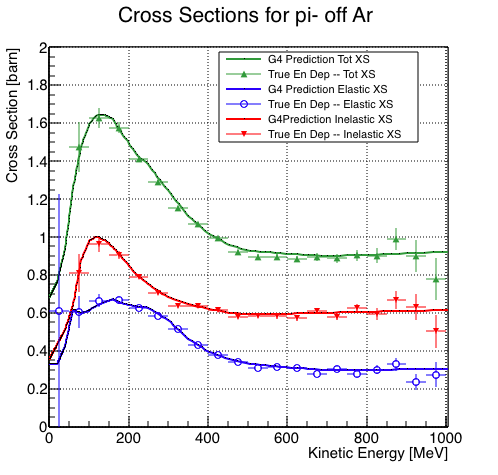
\includegraphics[width=3in]{Chapter-4/Images/PionTrueXS.png}
\end{minipage}%  
\begin{minipage}[b]{0.53\textwidth}  
  \centering  
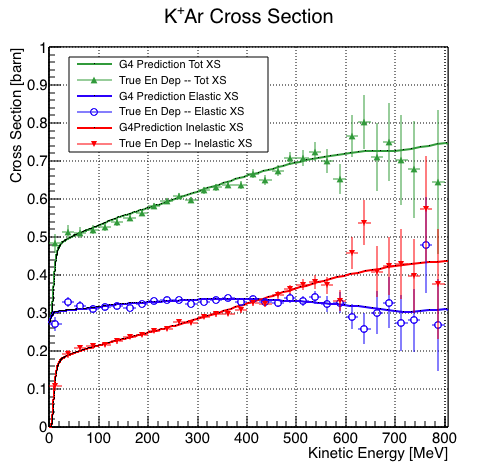
\includegraphics[width=3in]{Chapter-4/Images/KaonTrueXS.png}
\end{minipage}
\caption{Hadronic cross sections for ($\pi^-$,Ar) on the left and (K$^+$,Ar) on the right as implemented in Geant4 10.03.p1 (solid lines) overlaid the true MC cross section as obtained with the sliced TPC method (markers). The total cross section is shown in green,  the elastic cross section in blue and the inelastic cross section in red.}
\label{fig:TrueMCXS2}
\end{figure}
%\end{comment}






\chapter{Data and MC preparation for the Cross Section Measurements}\label{ch:samples}
%{\raggedleft ``\emph{Il dolce non lo mangi mai, ma qualche volta ti rifai.} \par}
%{\raggedleft \emph{Abbracciami}"\par}
%{\raggedleft -- Pietro Ciampi, L'amore e' tutto qui, 1971 -- \par}
%\vspace{0.5cm}

%{\raggedleft ``\emph{You never eat dessert, but, sometimes, you make up for it.} \par}
%{\raggedleft \emph{Hug me}"\par}
%{\raggedleft -- Pietro Ciampi, L'amore e' tutto qui, 1971 -- \par}
%\vspace{0.5cm}


This chapter describes the preparatory work done on the the data and Monte Carlo samples used for the cross section analyses. 
This entails the choice of the datasets and the production of the information needed to construct the Monte Carlo Simulation~(section \ref{sec:dataSet}),  the construction and use of said Monte Carlo simulation~(section \ref{sec:MCSet}), the study and optimization of the tracking in the TPC for the cross section analyses~(section \ref{sec:TrackingStudies}),  the calibration of the calorimetry response and related energy studies~(section \ref{ch:energyCal}). 



\section{Cross Section Analyses Data Sets}\label{sec:dataSet}
We choose LArIAT Run-II as the data period for the  ($\pi^{-}$,Ar) and (K$^{+}$,Ar) total hadronic cross section analyses. 
Data taking for the this period started on 03/15/2016  and ended on 07/31/2016. 
Since we are interested in beamline and TPC information, we ask basic requirements on the operational status of the time of fight, wire chambers and TPC to form the good run list for this period, which we informally call ``lovely runs".

The subset of lovely runs  chosen for the  ($\pi^{-}$,Ar) total hadronic cross section analysis includes only the -60A and -100A magnet configurations in negative polarity, even if LArIAT explored several other beamline configurations during Run-II. The -60A and -100A combined data set accounts for approximately 90\% of the total Run-II negative polarity runs.   The  choice of the main two beamline settings limits the need for the production of many MC sets and related corrections, still maintaining a high number of events. 
%Since the production of beamline Monte Carlo depends on the wanted beamline configuration, the choice of only two beamline settings limits the need for beamline MC production. 

Similarly, the subset of lovely runs chosen  for the (K$^{+}$,Ar)  total hadronic cross section analysis includes only the +60A and +100A magnet configurations in positive polarity. It should be noted that kaons are extremely rare in the +60A sample, thus the data sample for the (K$^{+}$,Ar) cross section after the mass selection is about 90\% +100A runs, as shown in Table \ref{tab:databreakdown}.

For the first measurements in LArIAT that uses both beamline and TPC information, we choose strict requirements on the reconstruction of the WC tracks, the so-called ``Picky Track" sample (see Section \ref{sec:MWPCfunc}). This choice presents two advantages:  the uncertainty on the momentum reconstruction for the ``Picky Tracks" sample is smaller compared to the ``High Yield" sample, and the comparison with the beamline MC results is straightforward. A possible future update and cross check of these analysis would be the use of the High Yield sample, where the statistics is about three times higher. 

The breakdown of beamline events as a function of the magnets settings is shown in Table \ref{tab:databreakdown}. 
The choice of the data sets determines the production of beamline MC and serves as basis for the production of Data Driven MC, as shown in the next sections.

\begin{table}[b]
\centering
\begin{tabular}{|l|c|c|c|}  
\hline
                                                              & I = 60 A          & I = 100 A   & Total     \\ \hline
Data Events after $\pi/\mu/e$ Mass Selection     &     67068          &  71413  & 138481 \\ \hline
Data Events after $K$ Mass Selection                &     274              &   2563   & 2837  \\ \hline
\end{tabular}
\caption{Number of data events which fit the $\pi/\mu/e$ or $K$ mass hypothesis as a function of magnet settings.}
\label{tab:databreakdown}
\end{table}



\section{Construction of a Monte Carlo Simulation for LArIAT}\label{sec:MCSet}
For the simulation of LArIAT events and for the simulation of the datasets' particle make up, we use a combination of two MC generators: the G4Beamline Monte Carlo and the Data Driven single particle Monte Carlo (DDMC). We use the G4Beamline MC to simulate the particle transportation in the beamline and calculate the particle composition of the beam just after the fourth Wire Chamber (WC4). In order to simulate the beamline particles after WC4 and in the TPC, we use the DDMC.

\subsection{G4Beamline}\label{ch:beamlineComposition}
G4Beamline simulates the beam collision with the LArIAT secondary target, the energy deposited by the particles in the LArIAT beamline detectors, and the action of the LArIAT magnets, effectively accounting for particle transportation through the beamline from the LArIAT target until ``Big Disk", a fictional, void detector located just before the LArIAT cryostat. 
 At the moment of this writing, G4Beamline does not simulated the responses of the beamline detectors. It is possible to interrogate the truth level information of the simulated particles in several points of the geometry. In order to ease the handshake between G4Beamline and the DDMC, we ask for the beam composition just after WC4.
Since LArIAT data are taken under different beam conditions, we need to simulate separately the beam composition according to the magnets' settings and the secondary beam intensity with G4Beamline. For the pion cross section analysis the relevant beam conditions are  secondary beam energy of 64 GeV, negative polarity magnet with current of 100 A and 60 A. For the kaon cross section analysis the relevant beam conditions is a secondary beam energy of 64 GeV, positive polarity magnet with current of 100 A. 

\subsubsection{Beam Composition for Negative Pion Cross Section}
Even if pions are by far the biggest beam component in negative polarity runs, the LArIAT tertiary beam is not a pure pion beam. While useful to discriminate between pions, kaons, and protons, the beamline detectors are not sensitive enough to  discriminate among the lighter particles in the beam: electrons, muons and pions fall under the same mass hypothesis. Thus, we need to assess the contamination from beamline particles other than pions in the event selections used for the pion cross section analysis and correct for its effects. The first step of this process is assessing the percentage of electrons and muons in the $\pi/\mu/e$ beamline candidates via the G4Beamline MC. 
Since the beamline composition is a function of the magnet settings, we simulate separately events for magnet current of -60A and -100A. 
Figure \ref{fig:BeamComposition} shows the momentum predictions from G4Beamline overlaid with data for the 60A runs (left) and for the 100A runs (right). The predictions for electrons, muons and pions have been staggered and their sum is area normalized to data. Albeit not perfect, these plots show a reasonable agreement between the momentum shapes in data and MC. We attribute  the difference in shape to the lack of simulation of the WC efficiency in the MC which is momentum dependent and leads to enhance the number events in the center of the momentum distribution.

\begin{figure}
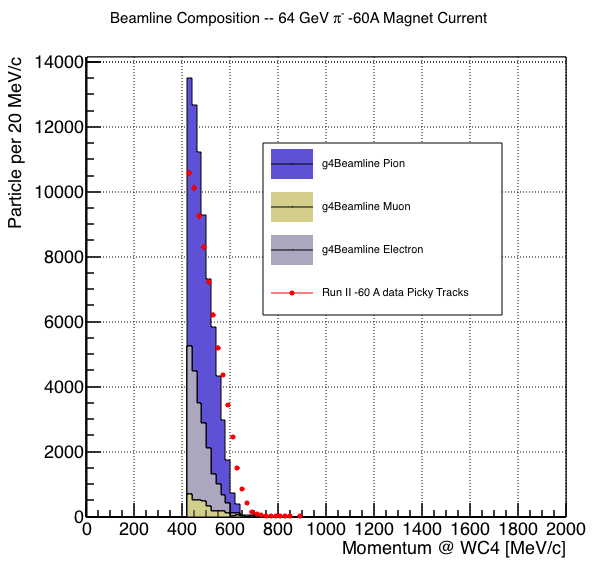
\includegraphics[width=0.5\textwidth,height=\textheight,keepaspectratio]{Chapter-5/Images/Beam60A.png}
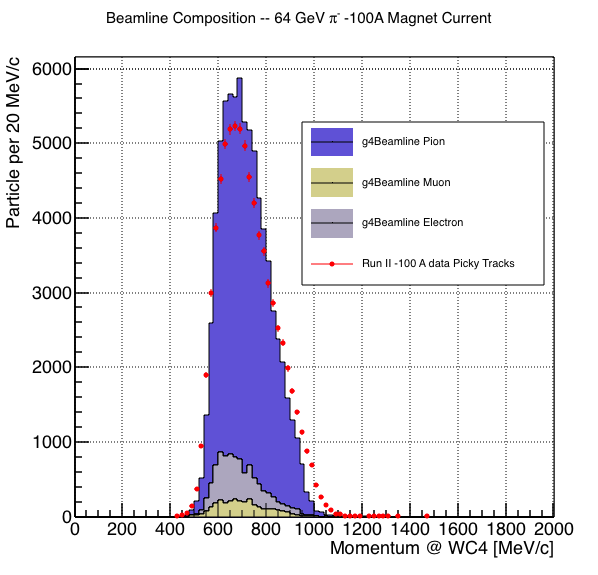
\includegraphics[width=0.5\textwidth,height=\textheight,keepaspectratio]{Chapter-5/Images/Beam100A.png}
\caption{Beam composition for the -60A runs (left) and -100A runs (right). The solid blue plot represents the simulated pion content, the yellow plot represents the simulated muon content and the grey plot represents the simulated electron content. The plots are area normalized to the number of data events, shown in red. }
\label{fig:BeamComposition}
\end{figure}

Table \ref{tab:beamline} shows the beam composition per magnet setting after the mass selection according to the G4Beamline simulation.
\begin{table}[]
\centering
\begin{tabular}{|l|c|c|}
\hline
                     & I = -60 A           & I = -100 A \\ \hline
G4Pions       &   68.8 \%           &      87.4 \%        \\ \hline
G4Muons     &     4.6 \%           &        3.7 \%         \\ \hline
G4Electrons &   26.6 \%           &        8.9 \%        \\ \hline
\end{tabular}
\caption{Simulated beamline composition per magnet settings}
\label{tab:beamline}
\end{table}

The estimated beam composition is used as a basis to estimate the background contamination in the  ($\pi^{-}$,Ar) cross section measurement, whose  full treatment is described in section \ref{ch:PionXSBkgSub}.

\subsubsection{Beam Composition for Positive Kaon Cross Section}
In the positive polarity runs, the tertiary beam composition is mainly pions and protons. The left side of Figure \ref{fig:BeamCompositionPos} shows the  predictions for the momentum spectra for the 100A positive runs  according to  G4Beamline (solid colors) overlaid with data (black points). 
Since the LArIAT beamline detectors can discriminate between kaons and other particles, we do not rely on the G4Beamline simulation to estimate the beamline contamination in the pool of kaon candidates (as in the case of the pion cross section), but rather we use a data drive approach. 
The basic idea of this data driven approach is to estimate the bleed over from high and low mass peaks under the kaon peak by fitting the tails of the $\pi/\mu/e$ and proton mass distributions, as shown in Figure \ref{fig:BeamCompositionPos} right side. 
Since the shape of the tails is unknown, the estimate is done multiple times varying the range and shape for reasonable functions. 
For example, to estimate the proton content under the kaon peak, we start by fitting the left tail of the proton mass distribution with a gaussian function between 650 $MeV/c^2$ and 750 MeV/c$^2$.% in a reasonable range and with a reasonable function. 
  We extend the fit function under the kaon peak and integrate the extended fit function between 350-650 MeV/c$^2$. We integrate the mass histogram in the same range and calculate the proton contamination as the ratio between the two integrals. We repeat this procedure for several fit shapes (gaussian, linear and exponential functions) and tail ranges. Finally, we calculate the contamination as the weighted average of single estimates, where the weights are calculated to be the $1./\chi^2$ of the tail fits. The procedure is repeated for lighter particles mass peak independently.
With 12 iterations of this method we find a proton contamination of  0.2 $\pm$ 0.5 \%  and a contamination from the lighter particles of 5 $\pm$ 2 \% .
The estimate of the proton background is currently not used in the kaon cross section analysis, but it is a fundamental step to retrieve the true kaon cross section which will be implemented in the analysis next step.


\begin{figure}
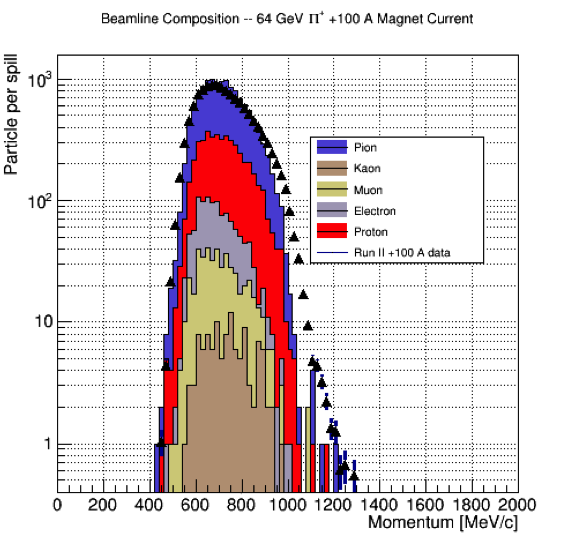
\includegraphics[width=0.5\textwidth,height=\textheight,keepaspectratio]{Chapter-5/Images/Beam100Pos.png}
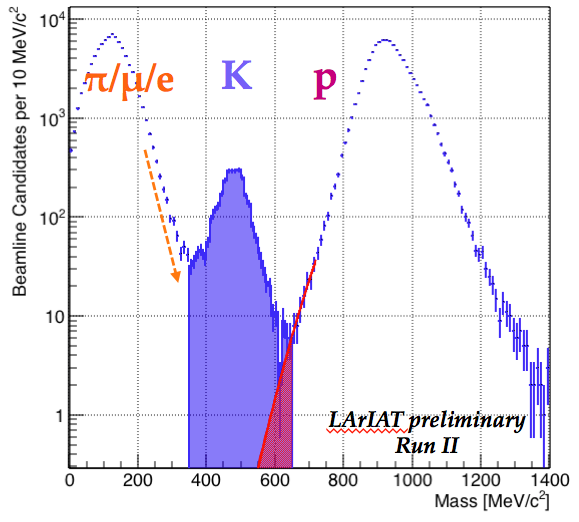
\includegraphics[width=0.5\textwidth,height=\textheight,keepaspectratio]{Chapter-5/Images/MassPos.png}
\caption{\emph{Left:} Beam composition for the +100A runs after WC4 (no mass selection applied). The solid colors represent the contributions from the G4Beamline simulated particles: blue plot represents the simulated pion content, the yellow plot represents the simulated muon content and the grey plot represents the simulated positron content, the red the proton content and the mustard the kaon content. The plots are area normalized to the number of data events, shown in black. \emph{Right:} Mass distribution for the Run-II positive runs, where the area under the kaon mass peak is highlighted in purple. The area under the extension of a possible fit for the proton tail is highlighted in red. }
\label{fig:BeamCompositionPos}
\end{figure}



\subsection{Data Driven MC}\label{sec:DDMC}
The Data Driven single particle Monte Carlo (DDMC) is a single particle gun which simulates the particle transportation from WC4 into the TPC leveraging on the beamline data information. The DDMC uses the data momentum and position at WC4 to derive the event generation: a general sketch of the DDMC workflow is shown in Figure \ref{fig:DDMCSketch}.

When producing a DDMC sample, beamline data from a particular running period and/or running condition are selected first. For example, data for the negative 60A runs and for the negative 100A runs inform the event generation stage of two different DDMC samples. Figure \ref{fig:DDMCQuantities}  schematically shows the data quantities of interest leveraged from data: the momentum ($P_x, P_y, P_z$) and position ($X, Y$) at WC4. For each data event, we obtain the  particle position ($X, Y$) at WC4 directly from the data measurement; we calculate the components of the momentum using the beamline measurement of the momentum magnitude in conjunction with the hits on WC3 and WC4 to determine the direction of the momentum vector, as described in section \ref{sec:MWPCfunc}. The momentum and position of the selected data form a 5-dimensional tupla, which we sample thousands of times through a 5-dimensional hit-or-miss sampling procedure to generate the MC events. This generates MC events  with the same momentum and position distributions as data, with the additional benefit of accounting for the correlations between the $P_x, P_y, P_z, X, Y$ variables.  As an example, the results of the DDMC generation compared to data for the kaon +100A sample are shown in figure \ref{fig:DDMCComparison} for the $P_z$, $X$ and $Y$ distributions; as expected, MC and data agree within the statistical uncertainty by construction. A LArSoft simulation module then launches single particle MC from z = -100 cm (the location of the WC4) using the MC generated events. The particles are free to decay and interact in their path from WC4 to the TPC according to the Geant4 simulation.

Using the DDMC technique ensures that the MC and data particles have very similar momentum, position and angular distributions at WC4 and allows us to use the MC sample in several occasions: to calibrate the energy loss upstream of the TPC (see Section \ref{ch:eloss}), to estimate the background contamination to the pion cross section (see Section \ref{ch:PionXSBkgSub}), or to study the tracking and the calorimetric performance (sections \ref{sec:TrackingStudies} and \ref{ch:energyCal}). A small caveat is in order here: the DDMC is a single particle Monte Carlo, which means that the beam pile-up is not simulated. 


Six samples are the basis fo the MC used in the pion cross section measurement: three samples of  $\sim$340000 pions, muons and electrons to simulate the negative 60A runs, and three samples of $\sim$340000 pions, muons and electrons for the negative 100A runs.

The MC used for the kaon cross section analysis is a sample of \textcolor{red}{NUMBERS}  kaons.

\begin{figure}[hpbt]
\centering
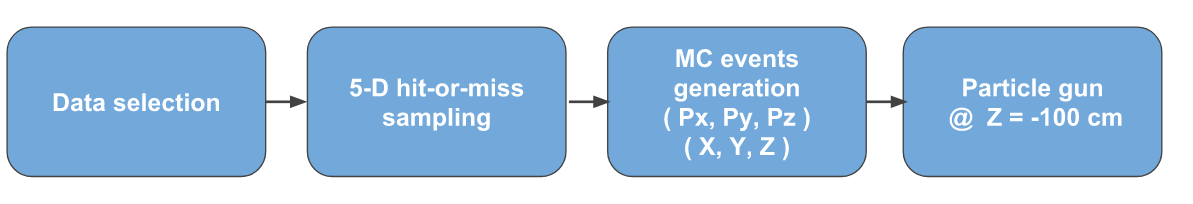
\includegraphics[width=\textwidth]{Chapter-5/Images/DDMCScheme.png}
\caption{Workflow for Data Driven single particle Monte Carlo production.}
\label{fig:DDMCSketch}
\end{figure}


\begin{figure}[hpbt]
\centering
\includegraphics[width=\textwidth]{Chapter-5/Images/DDMCQuantities.png}
\caption{Scheme of the quantities of interest for the DDMC event generation: $P_x, P_y, P_z, X, Y$ at WC4.}
\label{fig:DDMCQuantities}
\end{figure}


\begin{figure}[hpbt]
\centering
\includegraphics[width=0.48\textwidth]{Chapter-5/Images/DDMCPz.png}
\includegraphics[width=0.48\textwidth]{Chapter-5/Images/DDMCX.png}
\includegraphics[width=0.48\textwidth]{Chapter-5/Images/DDMCY.png}
\caption{Comparison between generated quantities and data distributions for the 100A kaon sample: Z component of the momentum at WC4 (top left), X position at Wire Chamber 4 (top right), Y position at Wire Chamber 4 (bottom).}
\label{fig:DDMCComparison}
\end{figure}





\section{Estimate of Backgrounds in the Pion Cross Section}\label{ch:PionXSBkgSub}

We use the beamline simulation and the DDMC simulation to estimate the background in the total hadronic pion cross section. Two categories of background exists for the negative pion cross section measurement: the one related to the pion interaction in the chamber, discussed in Section \ref{ch:CaptureAndDecay} and the one related to the beamline contamination, discussed in Section \ref{ch:PionXSBkgSub2}.

\subsection{Background from Pion Capture and Decay}\label{ch:CaptureAndDecay}
Our goal is to measure the total hadronic cross section for negative pions in argon. Since pion capture can be classified as an electromagnetic process and pion decay is a week process,  capture and decay represent unwanted interactions. We present here a study of capture and decay in Monte Carlo and the solution we adopted to mitigate their occurrence in the data sample. 

For this MC study, we use a sample of  MC pions generated according to the  $-6$0A beam profile with the DDMC (see Section \ref{sec:DDMC}). It is important to notice that capture occurs predominantly at rest, while decay may occur both in flight and at rest. Thus, we can highly mitigate capture and decay at rest by removing pions which would release all their energy in the TPC and stop. This translates into a momentum selection, where we keep only events whose WC momentum is above a certain threshold. 
Figure \ref{fig:CaptureMom} shows the true momentum distribution for the primary pions\footnote{We use here the Geant4 denomination ``primary" to indicate that the pion considered does not undergo interactions modifying its energy before getting to the TPC. In fact, not every pion shot from wire chamber four will arrive to the TPC as primary,  some will decay or interact before the TPC.}  that arrive to the TPC (pink), that capture (green) or decay (blue) inside the TPC, on a linear and log scale vertical axis. 




In order to choose the selection value for the wire chamber momentum, it is beneficial to estimate the ratio of events which capture or decay that survive the selection in MC as a function of the momentum threshold, and compare it with the survival ratio for all events. This is done in figure \ref{fig:survRatio}. We define the survival ratio simply  as the number of events surviving the true momentum selection divided by the number of events of that category. We calculate the survival ratio separately for the three event categories explained above: total (pink), capture (green) and decay (blue).
Selecting pions with momentum greater than 420 MeV/c reduces the capture events by ~99\% while maintaining about 80\% of the total data sample. 
Figure \ref{fig:evtRatio} shows the ratio of events which end their life in capture (green) or decay (blue) over the total number of events as a as a function of the true momentum at wire chamber four. This ratio is slightly dependent on the inelastic cross section implemented in Geant4, as we are able to register a pion capture (or decay) only if it did not interact inelastically in the TPC. We choose a momentum threshold of 420~MeV/c because the percentage of capture events drops below 1\% and the percentage of decays is never above 2\% for momenta greater than 420~MeV/c. After the momentum selection, we evaluate the contribution of capture and decay to be a negligibly small background to the cross section measurement compared to the background related to the beamline.

\begin{figure}[p]
\centering
\includegraphics[width=15cm]{Chapter-7/Images/CDAsMomentumFunct.png}
\caption{True momentum distribution at wire chamber 4 for every simulated pion arriving in the TPC (pink), ending its life in capture (green) or in decay (blue) in the TPC, linear vertical axis on the left, logarithmic on the right. }
\label{fig:CaptureMom}
\end{figure}

\begin{figure}[p]
\centering
\begin{minipage}[t]{0.45\textwidth}
\centering
\includegraphics[width=7.5cm]{Chapter-7/Images/CDThreshold.png}
\caption{Survival ratio as a function of selection threshold on true momentum at wire chamber four for for every simulated pion arriving in the TPC (pink), capture (green) or in decay (blue).   }
\label{fig:survRatio}
\end{minipage}\hfill
\begin{minipage}[t]{0.45\textwidth}
\centering
\includegraphics[width=7.5cm]{Chapter-7/Images/CDRatio.png}
\caption{Ratio between the capture (green) and decay (blue) events over the total number of events as a as a function of the true momentum at wire chamber four.}
\label{fig:evtRatio}
\end{minipage}
\end{figure}

\clearpage
%%%%%%%%%%%%%%%%%%%%%%%%%%%%%%%%%%%%%%%%%%%%%%%%%%%%%%%%%%%%
\subsection{Beamline Background}\label{ch:PionXSBkgSub2}
We define beamline background every TPC track matched to the WC track which is not a primary pion. Potentially, there are 4 different types of beamline background:
\begin{itemize}
\item[]1) electrons,
\item[]2) muons,
\item[]3) secondaries from pion events,
\item[]4) matched pile up events.
\end{itemize}

The first step is to estimate what percentage of events used in the cross section calculation is not a primary pion.  We start by noting that the last type of background, the ``matched pile up" events, is a negligible fraction, because of the definition of the WC2TPC match: we deem the probability of a single match with a halo particle in the absence of a beamline particle\footnote{ Events with multiple WC2TPC matches are always rejected.} negligibly small. %\textcolor{red}{SHOW VTX distribution in WC2TPC match}

As shown in Section \ref{ch:beamlineComposition}, we use G4Beamline to estimate the beam composition at WC4, obtaining the composition shown in Table \ref{tab:beamline}.
The next step to estimate the beamline background in the cross section measurement is propagating pions, muons and electrons to the TPC and evaluate their contribution to the cross section. To do so, we simulate the same number of electrons, muons and pions with the DDMC and we apply the same selection filters on the three samples. The number of events per particle species surviving this selection is shown on table \ref{tab:MCafterCutContaminants}.

Pions can travel the length of the LArIAT beamline and interact hadronically in the steel or in the non-instrumented argon upstream to the TPC front face. Or, they could decay in flight between WC4 and the TPC. One of the interaction products can leak into the TPC and be matched with the WC track, contributing to the pool of events used for the cross section calculation. We call this type of particles ``secondaries" from pion events, with a terminology inspired by Geant4. 
We estimate the number of secondaries using the DDMC pion sample.  The percentage of secondaries is given by the number of matched WC2TPC tracks whose corresponding particle is not flagged as primary by Geant4.  The secondary to pion ratio is 4.9\% in the 60A sample and 4.3\% in the 100A sample.


\begin{table}[]
\centering
\begin{tabular}{| l | l | l | l | l | l | l | l | }
\hline
 &  \multicolumn{3}{|c|}{Magnet Current -60A} & \multicolumn{3}{|c|}{Magnet Current -100 A}\\

                                                  & MC $\pi^-$   & MC  $ \mu^-$ & MC  $e^-$ & MC  $\pi^-$ & MC  $\mu^-$ & MC  $e^-$  \\
\hline
&  &  &  & & &\\  
Total Initial events                     & 334500  & 334500 & 334500 &344500 &344500& 344500 \\
After Multiplicity Rejection        & 330668  & 333420 & 198065 &326576 &344208& 201380 \\
After WC2TPC Selection          & 218239  & 296333 & 91139  &230418 &300228& 98834  \\
Evts After Shower Rejection     & 208063  & 288914 &  20293 &219882 &293585& 17780  \\
&  &  &  & & &\\  
  \hline
&  &  &  & & &\\  
Selection Survival Rate           &62.3\% & 86.6\% & 6.1\% & 63.8\%& 85.5\%& 5.2\%\\
Beam Composition  @WC4      &  68.8\%   &  4.6 \%  & 26.6 \%    & 87.4 \% & 3.7 \%  & 8.9 \% \\ %
Beam Composition  @TPC FF &  88.5\%   & 8.2\%   & 3.3 \%   & 94.0\%	& 5.3\% & 0.7\%\\
                                                  &                      &                       &                   &                       &                        &\\  
\hline
\end{tabular}
\caption{MC selection flow per particle species.}
\label{tab:MCafterCutContaminants}
\end{table}


\begin{figure}[p]
\centering
\includegraphics[width=\textwidth]{Chapter-5/Images/Background60A.pdf}
\caption{Left: staggered contributions to the interacting kinetic energy distribution for electron (grey), muons (yellow) and pion (blue) in the 60A simulation sample. Right: staggered contributions to the incident kinetic energy distribution for electron (grey), muons (yellow) and pion (blue) in the 60A simulation sample.  }
\label{fig:stag60A}
\end{figure}

In order to reproduce the closest make up of the beam to data, we weight each event of a given particle species according to the estimated beam composition. In case of 60A runs, for example, the weights are 0.688 for pions,  0.046 for muons  and 0.266 for electrons.
We produce accordingly the interacting and incident histograms for the events surviving the selection, staggering the contributions for each particle species, as shown in Figure  \ref{fig:stag60A}. From those histograms, we are able to evaluate the relative contribution of  pions and  background to each bin of the interacting and incident histograms separately and obtain the respective corrections for data. We take here the interacting histogram as example, noting that the derivation of the correction for the incident histogram is identical. The number of entries in each bin of the interacting plot (Figure \ref{fig:stag60A} left) is  $N^{\text{TOT}}_{\text{Interacting}} (E_{i})$, equal to the sum of the pions and background in that bin, namely

\begin{equation}
N^{\text{TOT}}_{\text{Interacting}} (E_{i}) =  N^\pi_{Interacting} (E_{i}) + \underbrace{ N^\mu_{Interacting} (E_{i}) + N^e_{Interacting} (E_{i}) + N^{Secondary}_{Interacting} (E_{i}) }_{B_{Interacting} (E_i)}.
\end{equation}
Thus, the relative contribution of pions to each bin in MC can be calculated as follows
\begin{equation}
C^{\pi MC}_{Interacting} (E_{i}) =  \frac{N^{\pi MC}_{Interacting}}{ N^{TOT MC}_{Interacting} (E_{i}) } =    \frac{N^{TOT MC}_{Interacting} (E_{i}) - B^ {MC}_{Interacting} (E_i)}{ N^{TOT MC}_{Interacting} (E_{i})}.
\end{equation}


In order to evaluate the pion content of each bin in data, we scale the measured bin content by the corresponding  pion contribution found in MC, as follows
\begin{equation}
N^{\pi Reco Data}_{Interacting} = N^{TOT Data}_{Interacting} (E_{i}) - B^{Data}_{Interacting} (E_i)  =  C^{\pi MC}_{Interacting} (E_{i}) N^{TOT Data}_{Interacting} (E_{i}).
\end{equation}


\section{Estimate of Energy Loss before the TPC}\label{ch:eloss}
The beamline particles travel a path from where their  momentum is measured in the beamline until they are tracked again inside the TPC. In the LArIAT geometry, a particle leaving the WC4 will encounter the materials listed in Table \ref{tab:budget} before being registered again. The energy lost by the particle in this non-instrumented material modifies the particle's kinetic energy and directly affects the cross section measurement, as shown in equation \ref{eq:enFF}.

\begin{table}[h!]
\centering
\begin{tabular}{|l|l|l|}
\hline
Material  & density {[}g/cm$^3${]} & width {[}cm{]}    \\ \hline
Fiberglass laminate (G10)      & 1.7                             & 1.28                              \\
Liquid Argon                           & 1.4                             & 3.20                             \\
Stainless Steel                        & 7.7                            & 0.23                             \\
Titanium                                  & 4.5                            & 0.04                             \\ 
Air                                            &  1.2 $\cdot10^{-3}$  & 89.43                              \\
Plastic Scintillator                    & 1.03                          & 1.20 (+ 1.30)                 \\ \hline
\end{tabular}
\caption{LArIAT material budget from WC4 to the TPC Front Face.}
\label{tab:budget}
\end{table}


We derive an estimate of the energy loss between the beamline momentum measurement and the TPC ($E_{loss}$) from the pion and kaon DDMC samples, since this quantity is not  measurable directly on data. 
The $E_{loss}$ distribution for the 60A  and 100A pion sample is shown in figure \ref{fig:ELoss60A}, left and right respectively. A clear double peaked structure is visible, which is due to the particles either missing or hitting the HALO paddle: a schematic rendering of this occurrence is  shown in figure \ref{fig:Halo}. The kinematic at WC4 determines the trajectory of a particle and whether or not it will hit the halo paddle. In figure \ref{fig:PxVsXTrue} , we plot the true  horizontal component of the momentum $P_x$ versus the true $X$ position at WC4 for pions missing the halo paddle (left) and for pions hitting the halo paddle (right) for the 60A MC simulation runs -- analogous plots are obtained with the 100A simulation. These distributions can be separated drawing a line in this position-momentum space. 
We use a logistic regression  \cite{agresti2013categorical}  as a classifier to find the best separating line, shown in both plots as the red line. We classify as ``hitting the halo paddle" all pions whose $P_x$ and $X$ are such that $$P_x +0.02* X - 0.4 < 0 $$ and as ``missing the halo  paddle" all pions whose $P_x$ and $X$ are such that $$P_x +0.02*X - 0.4 > 0, $$ where the coefficients of the line are empirically found by the logistic regression estimation. Overall, this simple method classifies in the right category (hit or miss) about 86\% of the pion events. In MC, we assign  $E_{loss} = 32 \pm 4 $~MeV for pion events classified as ``hitting the halo paddle"; we assign  $E_{loss} = 24 \pm 3 $~MeV for pion events classified as ``missing the halo paddle". We apply the same classifier on data. A scan of the simulated geometry showed an excess of 3 cm of uninstrumented argon compared with the surveyed detector geometry. We account for this difference by assigning in data $E_{loss} = 24 \pm 6 $~MeV for pion events classified as ``hitting the halo paddle" and  $E_{loss} = 17 \pm 6 $~MeV for pion events classified as ``missing the halo paddle", where the uncertainty is derived as the standard deviation of the double peaked distribution.

The summary of the values for used for $E_{Loss}$ for the pion sample is listed in table \ref{tab:Eloss}  with the analogous results for the study on the kaon case.

\begin{table}[b]
\centering
\begin{tabular}{|l|c|c|}  
\hline
                          &  \multicolumn{2}{c|}{E$_{loss}$ [MeV]}    \\ \hline
                          & Hitting Halo          & Missing Halo     \\ \hline
Pion  MC           &  $32 \pm 4 $         &    $24 \pm 3$     \\ \hline
Pion Data          &  $25 \pm 6$          &    $17 \pm 6 $    \\ \hline
Kaon  MC          &  $37 \pm 5 $        &     $31 \pm 4 $    \\ \hline
Kaon Data         &  $26 \pm 6 $        &     $22 \pm 6 $    \\ \hline
\end{tabular}
\caption{Energy loss for pions and kaons.}
\label{tab:Eloss}
\end{table}



%We use the separation of these two distributions to decide what the energy loss for each event on data. 
%Thus,  we assign the value for energy loss is used in the data.


\begin{figure}[hbpt]
\centering
\includegraphics[width=0.45\textwidth]{Chapter-5/Images/E_loss60A.png}
\includegraphics[width=0.45\textwidth]{Chapter-5/Images/E_loss100A.png}
\caption{True energy loss between WC4 and the TPC front face according to the MC simulation of negative pions of the 60A runs (left) and of the 100A runs (right). The distribution for the whole data sample is shown in blue, the distribution for the pions missing the halo is shown in red, and the distribution for the pions hitting the halo is shown in green.  }
\label{fig:ELoss60A}
\end{figure}

\begin{figure}[hbpt]
\centering
\includegraphics[scale=0.5]{Chapter-5/Images/Halo.png}
\caption{Schematic rendering of the particle path between WC4 and the TPC front face. The paddle with the hollow central circle represents the Halo paddle. We illustrate two possible trajectories: in black, a trajectory that miss the paddle and goes through the hole in the Halo, in blue a trajectory that hits the Halo paddle and goes through the scintillation material.}
\label{fig:Halo}
\end{figure}



\begin{figure}[hbpt]
\centering
\includegraphics[width=\textwidth]{Chapter-5/Images/PXVsX60A.png}
\caption{Horizontal component of the true momentum vs the horizontal position at WC4 for MC simulated pions of the 60A runs. The plot on the left shows the distribution for pion that miss the halo paddle and the plot on the right shows the distributions for pions that hit the halo. The form of the classifier is overlaid to both plots (red line).}
\label{fig:PxVsXTrue}
\end{figure}

\section{Tracking Studies}\label{sec:TrackingStudies}
In this section, we describe three studies. The first is a justification of the selection criteria for the beamline handshake with the TPC information.  We perform this study to boost  the correct identification of the particles in the TPC associated with the beamline information, while maintaining sufficient statistics for the cross section measurement.  The second study is an optimization of the tracking algorithm, with the scope of maximizing the identification of the hadronic interaction point inside the TPC.  These two studies are related, since the optimization of the tracking is performed on TPC tracks which have been matched to the wire chamber track; in turn, the tracking algorithm for TPC tracks determines the number of reconstructed tracks in each event used to try the matching with the wire chamber track. Starting with a sensible tracking reconstruction, we perform the WC2TPC matching optimization first, then the tracking optimization. The WC2TPC match purity and efficiency  are then calculated again with the optimized tracking.

The third study is an evaluation of  the angular resolution of the tracking algorithm in data and MC, which is particularly important in the context of the cross section analyses.



\subsection{Study of WC to TPC Match}\label{ch:WC2TPCMatchOptimization}

Plots I want in this section:
\begin{enumerate}
\item WC2TPC MC DeltaX, DeltaY and $\alpha$
\end{enumerate}


Scope of this study is assessing the goodness of the wire chamber to TPC match on Monte Carlo and decide the selection values we will use on data. A word of caution is necessary here. With this study, we want to minimize pathologies associated with the presence of the primary hadron itself, e.g. the incorrect association between the beamline hadron and its decay products inside the TPC.  Assessing the contamination from pile-up\footnote{We remind the reader that the DDMC is a single particle Monte Carlo, where the beam pile up is not simulated.}, albeit related, is beyond the scope of this study.

In MC, we are able to define a correct WC2TPC match using the Geant4 truth information. We are thus able to count how many times the WC tracks is associated with the wrong TPC reconstructed track. 

We define a correct match if the all following conditions are met:
\begin{itemize}
\item[-] the length of the true primary Geant4 track in the TPC is greater than 2 cm,  
\item[-] the length of the reconstructed track length is greater than 2 cm,
\item[-] the Z position of the first reconstructed point is within 2 cm from the TPC front face
\item[-] the distance between the reconstructed track and the true entering point is the minimum compared with all the other reconstructed tracks.
\end{itemize}

In order to count the wrong matches, we consider all the reconstructed tracks whose Z position of the first reconstructed point lies within 2 cm from the TPC front face. Events with true length in TPC $<$ 2 cm are included. 
Since hadrons are shot 100 cm upstream from the TPC front face, the following two scenarios are possible from a truth standpoint: 
\begin{itemize}
\item[[$Ta$]] the primary hadron decays or interact strongly before getting to the TPC,
\item[[$Tb$]] the primary hadron enters the TPC.
\end{itemize}

As described in Section \ref{ch:WC2TPCMatchMethod}, we define a WC2TPC match according to the relative position of the WC and TPC track parametrized with $\Delta R$ and the angle between them, parametrized with $\alpha$. Once we choose the selection values $r_{T}$ and $\alpha_{T}$ to determine a reconstructed WC2TPC match, the following five scenarios are possible in the truth to reconstruction interplay : 
\begin{itemize}
\item[1)] only the correct track is matched
\item[2)] only one wrong track is matched 
\item[3)] the correct track and one (or more) wrong tracks are matched
\item[4)] multiple wrong tracks  matched.
\item[5)] no reconstructed tracks are matched
\end{itemize}

Since we keep only events with one and only one match, we discard cases 3), 4) and 5) from the events used in the cross section measurement. For each set of $r_{T}$ and $\alpha_{T}$ selection value, we define purity and efficiency of the selection as follows:
\begin{equation}
\text{Efficiency} = \frac{\text{Number of events correctly matched}}{\text{ Number of events with primary in TPC}},
\end{equation}

\begin{equation}
\text{Purity} = \frac{\text{Number of events correctly matched}}{\text{Total number of matched events}}.
\end{equation}

Figure \ref{fig:EffPurityK} shows the efficiency (left) and purity (right) for WC2TPC match as a function of the radius, $r_{T}$, and angle, $\alpha_{T}$, selection value. It is apparent how both efficiency and purity are fairly flat as a function of the radius selection value at a given angle. This is not surprising. Since we are studying a single particle gun Monte Carlo sample, the wrong matches can occur only for mis-tracking of the primary or for association with decay products;  decay products will tend to be produced at large angles compared to the primary, but could be fairly close to the in $x$ and $y$ projection of the primary. The radius cut would play a key role in removing pile up events. 

For LArIAT cross section measurements, we generally prefer purity over efficiency, since a sample of particles of a pure species will lead to a better measurement. Obviously, purity should be balanced with a sensible efficiency to avoid rejecting the whole sample. 

We choose $(\alpha_{T}$, $r_{T}) = (8 \text{ deg}, 4 \text{ cm} )$ and get a MC 85\% efficiency and 98\% purity for the kaon sample and a MC 95\% efficiency and 90\% purity for the pion sample.


\begin{figure}[hpbt]
\centering
\includegraphics[width=15cm]{Chapter-5/Images/KEffPurity.png}
\caption{Efficiency (left) and purity (right) for WC2TPC match as a function of the radius and angle selections for the kaon sample.}
\label{fig:EffPurityK}
\end{figure}




\subsection{Tracking Optimization}\label{ch:TrackOptimization}


\subsection{Angular Resolution}\label{sec:angleRes}
Scope of this study is to understand and compare the tracking performances and angular resolution of the TPC tracking on data and MC. 
We use the angular resolution of the tracking to determine  the value of smallest angle that we can reconstruct with a non-zero efficiency, effectively determining a selection on the angular distribution of the cross section measurement due to the tracking performance. This study is performed on the pion sample, but its results are extrapolated to the kaon case.

We start by selecting all the WC2TPC matched tracks used for the cross section analysis.  These tracks can contain from a minimum of 3 3D-space points to a maximum of 240  3D-space points.  We fit a line to all the 3D-space points associated with the track. 
For each track we calculate the average distance between each point in space and the fit line as follows 
\begin{equation} 
\bar d = \frac{\sum^N_i d_i}{N},
\end{equation} 
where $N$ is the number of 3D-space points of the track and $d_i$ is the distance of the $i$-th space point to the line fit. Several tests to compare the goodness of fit between data and MC have been considered. We decided to use $\bar d$ for its straightforward interpretation. The $\bar d$ distribution for data and MC is shown in Figure \ref{fig:Chi2AllPts} and shows a relatively good agreement between data and MC.

A visual representation of the procedure used to evaluate the angular resolution is shown in Figure \ref{fig:AngResProcedure}. 
For each track, we order the space points according to their Z position along the positive beam direction (panel a) and we split them in two sets: the first set contains all the points belonging to the first half of the track and the second set contains all the points belonging the second half of the track. We remove the last four points in the first set and the first four points in the second set, so to have a gap in the middle of the original track (panel b). We fit the first and the second set of points with two lines  (panel c). We then calculate the angle between the fit of the first and second half $\alpha$ (panel d). The angle $\alpha$ determines the spatial resolution of the tracking. The distributions for data and MC for $\alpha$ are given in Figure \ref{fig:trackingResolution}. The mean of the data and MC angular resolution are respectively 

\begin{equation}
\bar\alpha_{Data} = (5.0 \pm 4.5) \text{ deg}, 
\end{equation}

\begin{equation}
\bar\alpha_{MC} = (4.5 \pm 3.9) \text{ deg}. 
\end{equation}

Interaction angles smaller than the angle resolution are indistinguishable for the reconstruction. Therefore, we assess our ability to measure the cross section to be limited to interaction angles greater than 5.0 deg. More accurate studies of the angular resolution as a function of the kinetic energy and track length, albeit interesting, are left for an improvement of the analysis. 

It is beneficial to take a moment to describe the definition of interaction angle. In case of elastic scattering, the definition is straightforward: the interaction angle is the angle between the incoming and outgoing pion, i.e.

\begin{equation}  
\theta = \cos^{-1} \Big(\frac{\vec p _{\text{incoming}}  \cdot\vec p _{\text{outgoing}}}{|\vec p _{\text{incoming}}|  |\vec p _{\text{outgoing}}| }\Big).
\end{equation}   
In case of inelastic scattering,  the presence of several topologies requires a more complex definition, as shown in figure \ref{fig:scatterPic}.  We define the scattering angle as the biggest of the angles between the incoming pion and the visible daughters, where the visible daughters are charged particles that travel more than 0.47 cm in the detector (see panel a); in case all the daughters are invisible, the angle is assigned to be 90 deg (see panel b). We chose this working definition of scattering angle for inelastic scattering keeping in mind how our tracking reconstruction works: the tracking will stop correctly in case of all the daughters are not visible in the detector and it is likely to stop correctly if multiple daughters form an interaction vertex. The only ``dangerous" case is the production of one charged daughter plus neutrals, which we can study with this working definition of scattering angle (see panel c).


We can see the effects of the angular resolution on the cross section by plotting the true Geant4 cross section for interaction angles greater than a minimum interaction angle. Figure \ref{fig:trueWithAngles} shows the  true Geant4 cross section  for interaction angles greater than 0 deg (green), 4.5 deg (red), 5.0 deg  (blue) and 9.0 deg (yellow). 
A small $0.5 \text{ deg}$ systematic shift between the mean of the data and MC angular resolution is present.%, which we account for in the context of the MC efficiency correction to the cross section, as presented in \ref{sec:angSys}.

\begin{figure}[ht]
\begin{minipage}[t]{0.45\linewidth}
\centering
\includegraphics[width=\textwidth]{Chapter-5/Images/cDAvg.png}
\caption[]{Distributions of the average distance between each 3D point in space and the fit line,  $\bar d$ for the data used in the pion cross section analysis and the pion only DDMC. The distributions are area normalized. } \label{fig:Chi2AllPts}
\end{minipage}
\hspace{0.5cm}
\begin{minipage}[t]{0.45\linewidth}
\centering
\includegraphics[width=\textwidth]{Chapter-5/Images/cTrackingDeg.png}
\caption[]{Distributions of angular resolution $\alpha$ for data used in the pion cross section analysis and pion only DDMC. The distributions are area normalized. } \label{fig:trackingResolution}
\end{minipage}
\end{figure}




\begin{figure}[ht]
\begin{minipage}[t]{0.45\linewidth}
\centering
\includegraphics[width=\textwidth]{Chapter-5/Images/TrackingProcedure.png}
\caption{A visual representation of the procedure used to evaluate the angular resolution.}
\label{fig:AngResProcedure}
\end{minipage}
\hspace{0.5cm}
\begin{minipage}[t]{0.45\linewidth}
\centering
\includegraphics[width=\textwidth]{Chapter-5/Images/Daughters.png}
\caption{A visual representation of the scattering angle definition in case of inelastic scattering.}
\label{fig:scatterPic}
\end{minipage}
\end{figure}

\begin{figure}[p]
\centering
\includegraphics[width=0.48\textwidth]{Chapter-5/Images/cTrueXSAngle.png}
\caption{ True ($\pi^-, Ar$) cross section for interaction angles greater than 0 deg (green), 4.5 deg (red), 5.0 deg  (blue) and 9.0 deg (yellow). }
\label{fig:trueWithAngles}
\end{figure}



\clearpage
%%%%%%%%%%%%%%%%%%%%%%%%%%%%%%%%%%%%%%%%%%%%%%%%%%%%%%%%%%%%%%
%%%%%%%%%%%%%%%%%%%%%%%%%%%%%%%%%%%%%%%%%%%%%%%%%%%%%%%%%%%%%%
%%%%%%%%%%%%%%%%%%%%%%%%%%%%%%%%%%%%%%%%%%%%%%%%%%%%%%%%%%%%%%

\section{Calorimetry Studies}\label{ch:energyCal} 
The ability to measure the kinetic energy of hadrons in the TPC is fundamental for the cross section analyses. 
Thus, we describe first how we calibrate the TPC calorimetric response (Section \ref{ch:energyCalibration}) and how we measure the kinetic energy of the hadrons in the TPC (Section \ref{ch:kinEn}).

\subsection{Energy Calibration}\label{ch:energyCalibration}
Scope of the energy calibration is to identify the factors which convert the charge collected (dQ) to energy deposited in the chamber (dE). As described in section \ref{sec:SignalProc}, this is a multi-step procedure. In LArIAT, we first correct the raw charge by the electronic noise on the considered wire \cite{LArIATdqdx}, then by the electron lifetime \cite{LArIATLifeTime},  and then by the recombination using the ArgoNeut recombination values. Lastly, we apply overall calibration of the energy, i.e. we determine the ``calorimetry constants" using the procedure described in this section.


We independently determine  the calorimetry constants for Data and Monte Carlo in the LArIAT Run-II Data samples using  a parametrization of the stopping power (a.k.a. energy deposited per unit length, $dE/dX$)  as a function of momentum. This is done by comparing the stopping power measured on reconstructed quantities against the Bethe-Bloch theoretical prediction for various particle species (see Equation \ref{eq:BB}).  We obtain the theoretical expectation for the $dE/dX$ most probable value of pions ($\pi$), muons ($\mu$), kaons ($K$), and protons ($p$) in the momentum range most relevant for LArIAT (Figure \ref{fig:PDGEnergyLossArgon}) using the tables provided by the Particle Data Group \cite{Patrignani:2016xqp} for liquid argon \cite{PDG-Argon}.

The basic idea of this calibration technique is to utilize a sample of beamline events with known particle species and momentum to measure the $dE/dX$ of the corresponding tracks in the TPC. In particular, we decided to use positive pions as calibration sample and samples from all the other particle species as cross check. Once the $dE/dX$ of the positive pion sample  has been measured at various momenta, we tune to calorimetry constants within the reconstruction software to align the measured values to match the theoretical ones found in Figure \ref{fig:PDGEnergyLossArgon}. 

In data, we start by selecting a sample of beamline positive pion beamline candidates without any restriction on their measured momentum\footnote{it should be noted that some muon and position contamination is present in the $\pi^+$ sample}.
We then apply the WC2TPC match and subtract the energy loss upstream to the TPC front face, determining the momentum at the TPC front face. For each surviving pion candidate,  we measure the $dE/dx$ at each of the first 12 spacepoints associated the 3D reconstructed track, corresponding to a $\sim$ 5 cm portion. These $dE/dX$ measurements are then put into a histogram that corresponds to measured momentum of the track. The $dE/dX$ histograms are sampled every 50 MeV/c in momentum (e.g. 150~MeV/c $< P <$ 200~MeV/c, 200~MeV/c $< P <$ 250/c~MeV, etc...).   This process of selecting, sampling, and recording the $dE/dX$ for various momentum bins is repeated over the entire sample of events, allowing us to collect sufficient statistic in most of the momentum bins between 150~MeV/c and 1100~MeV/c. On average, pions and muons only lose $\sim$10 MeV in this 5~cm section of the track and protons lose $\sim$20 MeV. Thus choosing 50 MeV/c size bins for our histograms covers the energy spread within those bins due to energy loss from ionization for all the particle species identifiable in the beamline. 
Each 50 MeV/c momentum binned $dE/dX$ histogram is now fit with a simple Landau function. The most probable value (MPV) and the associated error on the MPV from the fit are extracted and plotted against the theoretical prediction Figure \ref{fig:PDGEnergyLossArgon}. Depending on the outcome of the data-prediction comparison, we modify the calorimetry constants and we repeat the procedure until a qualitative agreement is achieved.  We perform this  tuning for the collection and induction plane separately. 
As a cross check to the calorimetry constants determined using the positive pions, we lock the constants and  plot the $dE/dx$ versus momentum distribution of all the other particle species identifiable in the beamline data ($\pi/\mu/e$, K , p, in both polarities) against the corresponding Beth-Bloch prediction. The agreement between data from the other particle species and the predictions is the expected result of this cross check.
The results of the tuning and cross check for Run-II data on the collection plane is shown in Figure \ref{fig:BBandData}  negative polarity data on top, positive polarity data on the bottom.

In MC, we simulate the corresponding positive pion sample with the DDMC (see section \ref{sec:DDMC}) and follow the same steps as in data. More details on the calorimetry tuning can be found in \cite{LArIATCalo}.

\textcolor{red}{Add agreement between data and MC for dedx for pions}

\begin{figure}[htb]
\centering
\includegraphics[width=0.50\textwidth]{Chapter-5/Images/dEdXvsMomentumTemplate.png}
\caption{Stopping power for pions, muons, kaons, and protons in liquid argon over the momentum range most relvant for LArIAT according to the Beth-Bloch equation. The solid lines represent the prediction for the mean energy $dE/dX$, while the dashed lines are the predictions for the MPV.}
\label{fig:PDGEnergyLossArgon}
\end{figure}


\begin{figure}[htb]
\centering
\includegraphics[width=0.50\textwidth]{Chapter-5/Images/RunIINegTotaldEdXvsMomentum.png}
\includegraphics[width=0.50\textwidth]{Chapter-5/Images/RunIIPosTotaldEdXvsMomentum.png}
\caption{Stopping power versus Momentum for Run-II negative (top) and positive (bottom) polarity data. We achieve the agreement between the Bethe-Bloch predictions and the distribution obtained with of the positive pions (top plot, red dots) by tuning the calorimetry constants. Once the calorimetry constants are locked in, the agreement between the other particle species and the Bethe-Bloch predictions follows naturally.}
\label{fig:BBandData}
\end{figure}


%\begin{figure}[htb]
%\centering
%\includegraphics[width=0.50\textwidth]{images/CalibrationExample.png}
%\caption{Illustration of the calibration technique. Here we depict a 325 MeV wire chamber track (shown in green) which enters the TPC (taking into account the energy loss from the upstream material) and we sample the first 12 spacepoints (shown in teal) to extract the dE/dX distribution which is fit with a Landau.}
%\label{fig:CalibrationExample}
%\end{figure}






\subsection{Kinetic Energy Measurement}\label{ch:kinEn}
The measured kinetic energy of a hadron candidate at each argon slab determines which bins of the interacting and incident histograms a selected event is going to fill. In this section, we define the measurement on the kinetic energy and  determine the related uncertainty. We will propagate this uncertainty into the cross section measurement, as discussed in Section \ref{ch:SysUncertaintyXSRaw} for the pion cross section and in Section \ref{ch:SysUncertaintyXSRawKaon} for the kaon cross section.

The kinetic energy of a hadron at the $j^{\text{th}}$ slice of argon in the TPC is given by

\begin{equation}
KE_{j} = \sqrt{p_{Beam}^2 + m_{Beam}^2} - m_{Beam}^2 - E_{Loss} - E_{\text{FF-j}},
\end{equation}

where $p_{Beam}$ is the momentum measured by the beamline detectors,  $m_{Beam}$ is the mass of the hadron as reported in the PDG,  $E_{Loss}$  is the energy loss between the beamline and the TPC, and $ E_{\text{FF-j}}$ is the energy that the hadron deposited from the TPC front face until the $j^{\text{th}}$ slice.
The uncertainty on $KE_{j}$ is then given by 
\begin{equation}
\delta KE_{j} = \sqrt{\delta p_{Beam}^2 + \delta E_{Loss}^2 +  \delta  E_{\text{dep FF-j}}^2},
\end{equation}

where we have dropped the uncertainty on the mass, since it is orders of magnitude smaller than the other uncertainties.
We assume the relative uncertainty on $p_{Beam}$ to be 2\%, and the uncertainty on the energy loss upstream to be 7~MeV, as calculated in Section \ref{ch:eloss}. We describe the estimate of the uncertainty on $E_{\text{FF-j}}$ in the rest of this section.

The energy deposited by the hadron from the TPC front face until the $j^{\text{th}}$ slice is the sum of the measured energy deposited in each previous slabs $E_{i}$, i.e.
\begin{equation}
E_{\text{FF-j}} = \sum_{i<j} E_{i}, 
\end{equation}
where $E_{i}$ is measured in each slab as  the product of the stopping power,  $dE/dX_{i}$,  and the track pitch, $Pitch_i$, for that point. 
If we assume conservatively that the measurements of $E_{i}$ are not independent from one another, the uncertainty on $E_{\text{FF-j}}$ becomes
\begin{equation}
\delta E_{\text{FF-j}} = (j-1) \delta E_{i}, 
\end{equation}
where $\delta E_{i}$ is the uncertainty on the energy loss in one slab of argon.

The left side of Figure \ref{fig:EnergyDeposited} shows the distribution of the energy deposited in each slab of argon, for the 60A negative pion dataset in black and for the pion only MC in blue. The analogous plot for the -100A negative pion data set  is show on the right side of Figure \ref{fig:EnergyDeposited}.  The distributions are fitted with a landau displayed in red for data and in teal for MC.
The uncertainty on $E_{i}$ is given by the width of the Landau fit to the data. A small systematic uncertainty  is given by a 1.0\% difference between the most probable value of the landau fits in data and MC.

\begin{figure}[htb]
\centering
\includegraphics[width=0.48\textwidth]{Chapter-5/Images/DepEnergy_Fit_v4.png}
\includegraphics[width=0.48\textwidth]{Chapter-5/Images/DepEnergy_Fit_v4100A.png}
\caption[]{ Energy deposited  $E_{i}$ in a single slab of argon for the pion -60A runs (left) and -100A runs (right).  The data is shown in black, the MC in blue. The distributions are fitted with a landau displayed in red for data and in teal for MC. } \label{fig:EnergyDeposited}
\end{figure}


\begin{comment}

Figure \ref{fig:EnergyDepositedStacked} shows the stacked version of the Energy Deposited plots with the backgrounds stacked. The backgrounds are given in the ratio of 68.8\% pion, 4.6\% muon, and 26.6\% electron. Once they are taken in these ratios, the sum of the MC is normalized to the sum of the data.

\begin{figure}[htb]
\centering
\includegraphics[width=0.48\textwidth]{Chapter-5/Images/DepEnergy_Stacked_v1.png}
\includegraphics[width=0.48\textwidth]{Chapter-5/Images/DepEnergy_Stacked_v3.png}
\caption[]{ Energy Deposited with all the MC and 60A data.  } \label{fig:EnergyDepositedStacked}
\end{figure}

The energy at the interacting point is given by
\begin{equation}
KE_{Interaction} = \sqrt{P_{WCtrk}^2 + m_{\pi}^2} - E_{Loss} - (\Sigma dE/dX_{i} \times Pitch)
\end{equation}

and has the exact same uncertainty as the incident kinetic energy plot. Thus these estimates can be applied to getting the uncertainty on the energy of the reconstructed cross-section.




%%%%%%%%%%%%%%%%%%%%%%%%%%%%%%%%%%%%%%%%%%%%%%%
\subsection{dE/dX}
%%%%%%%%%%%%%%%%%%%%%%%%%%%%%%%%%%%%%%%%%%%%%%%
Figure \ref{fig:dEdXLinearScale} shows the output of the fit of the Pion MC and the 60 Amp data. The MC is normalized to the data and both are fit to a Landau function. \footnote{The entries at dE/dX = 0 come from an uninitialized variable and can/should be taken out of these plots}

\begin{figure}[htb]
\centering
\includegraphics[width=0.48\textwidth]{Chapter-5/Images/dEdX_Fit_v1.png}
\includegraphics[width=0.48\textwidth]{Chapter-5/Images/dEdX_Fit_v4.png}
\caption[]{ dE/dX for 60Amp data and data driven pion MC, both fit with a Landau  } \label{fig:dEdXLinearScale}
\end{figure}

The difference between the two MPV's, is 2.4\% between the data and the MC.

Figure \ref{fig:dEdXLinearStacked} shows the stacked version of the dE/dX with the backgrounds stacked. The backgrounds are given in the ratio of 68.8\% pion, 4.6\% muon, and 26.6\% electron. Once they are taken in these ratios, the sum of the MC is normalized to the sum of the data.

\begin{figure}[htb]
\centering
\includegraphics[width=0.48\textwidth]{Chapter-5/Images/dEdX_stacked_v1.png}
\includegraphics[width=0.48\textwidth]{Chapter-5/Images/dEdX_stacked_v4.png}
\caption[]{ Stacked versions of the dE/dX with the data and electron/muon/pion MC.  } \label{fig:dEdXLinearStacked}
\end{figure}

For completeness, the log scale versions of are shown in Figure \ref{fig:dEdXLogScale}.

\begin{figure}[htb]
\centering
\includegraphics[width=0.48\textwidth]{Chapter-5/Images/dEdX_Fit_v2.png}
\includegraphics[width=0.48\textwidth]{Chapter-5/Images/dEdX_Fit_v3.png}
\includegraphics[width=0.48\textwidth]{Chapter-5/Images/dEdX_stacked_v2.png}
\includegraphics[width=0.48\textwidth]{Chapter-5/Images/dEdX_stacked_v3.png}
\caption[]{ dE/dX for 60Amp data and MC shown in log scale  } \label{fig:dEdXLogScale}
\end{figure}



%%%%%%%%%%%%%%%%%%%%%%%%%%%%%%%%%%%%%%%%%%%%%%%
\subsection{Energy Deposited}\label{sec:Energy}
%%%%%%%%%%%%%%%%%%%%%%%%%%%%%%%%%%%%%%%%%%%%%%%




\end{comment}





\chapter{Negative Pion Cross Section Measurement}\label{ch:PionXS}
{\raggedleft ``\emph{Y ella es flama que se eleva, Y es un p\'ajaro a volar.} \par}
{\raggedleft \emph{En la noche que se incendia, estrella de oscuridad}\par}
{\raggedleft \emph{que busca entre la tiniebla, la dulce hoguera del beso.}"\par}
{\raggedleft -- Lila Downs, Benediction And Dream,  2002 -- \par}
\vspace{0.5cm}

In this chapter, we show the result of the thin slice method to measure 
the ($\pi^-$-Ar) total hadronic cross section. In Section \ref{ch:PionXSRaw}, we start by measuring the raw cross section, i.e. the cross section obtained exclusively using data reconstruction, without any additional corrections. In Section \ref{ch:PionXSCorrections}, we apply a statistical subtraction of the background contributions based on simulation and a correction for detection inefficiency. The final results are presented in Section \ref{ch:FinalPion}.


\section{Raw Cross Section}\label{ch:PionXSRaw}
We measure the raw ($\pi^-$-Ar) total hadronic cross section as a function of the kinetic energy in the two chosen data sets, the -60A and -100A negative runs. 
As we will clarify in Section \ref{ch:PionXSCorrections},  the corrections to the raw cross section depend on the beam conditions and need to be calculated independently for the two datasets. Thus, we present here the measurement of the raw cross section on the two datasets separately.


As stated in section \ref{ch:XSRaw},  the raw cross section is given by the equation \ref{eq:thinTargetXSSolved}
\begin{equation}
 \sigma_{TOT} (E_i)  = \frac{1}{n \delta X}\frac{N^{\text{TOT}}_{\text{Int}}(E_i)}{N^{\text{TOT}}_{\text{Inc}}(E_i)},
\end{equation}

where $N^{\text{TOT}}_{\text{Int}}$  is the measured number of particles interacting at kinetic energy $E_i$, $N^{\text{TOT}}_{\text{Inc}}$ is the  measured  number of particles incident  on an argon slice at  kinetic energy $E_i$,  $n$ is the density of the target centers  and $\delta X$ is the thickness of the argon slice. The density of the target centers and the slab thickness are $n = 0.021\cdot10^{24} \text{ cm}^{-3} $ and  $\delta X=0.47\text{ cm}$, respectively.


Figure \ref{fig:InteractingRaw} shows the distribution of  $N^{\text{TOT}}_{\text{Int}}$  as a function of the kinetic energy for the 60A dataset on the left and for the 100A dataset on the right. The data central points are represented by black dots, the statistical uncertainty is shown in black, while the systematic uncertainty is shown in red. Data is displayed over the $N^{\text{TOT}}_{\text{Int}}$  distribution obtained with a MC mixed sample of pions, muon and electrons (additional details on the composition will be provided in Section \ref{ch:BKGsubXS}). The contribution from the simulated pions is shown in blue, the one from secondaries in red, the one from muons in yellow and the ones from electrons in gray. 
The simulated pion's and backgrounds' contributions are stacked; the sum of the integrals from each particle species is normalized to the integral of the data.
 
Figure \ref{fig:IncidentRaw} shows the distribution of  $N^{\text{TOT}}_{\text{Inc}}$   for the 60A dataset on the left and for the 100A dataset on the right. Data is displayed over the MC. The same color scheme and normalization procedure is used for both the interacting and incident histograms. 


Figure \ref{fig:XSRaw} shows the raw cross section for the 60A dataset on the left and for the 100A dataset on the right, statistical uncertainty in black and systematic uncertainty in red. The raw data cross section is overlaid to the reconstructed cross section for the MC mixed sample, displayed in azure. Since the background contributions and the detector effects for the 60A and 100A sample are different, it is premature to compare the raw cross sections obtained from the two samples at this point.

We describe the calculation of the statistical uncertainty for the interacting, incident and cross section distributions in Section \ref{ch:StatUncertaintyXSRaw}; we describe the procedure to calculate the corresponding systematics uncertainty on Section \ref{ch:SysUncertaintyXSRaw}.

\begin{figure}[p]
\centering  
\includegraphics[width=0.48\textwidth]{Chapter-6/Images/Plots60A_MCData_Int_StatSyst.pdf}
\includegraphics[width=0.48\textwidth]{Chapter-6/Images/Plots100A_MCData_Int_StatSyst.pdf}
\caption{Raw number of interacting pion candidates as a function of the reconstructed kinetic energy for the 60A runs (left) and for the 100A runs (right). The statistical uncertainties are shown in black, the systematic uncertainties in red.}
\label{fig:InteractingRaw}
\end{figure}


\begin{figure}
\centering  
\includegraphics[width=0.48\textwidth]{Chapter-6/Images/Plots60A_MCData_Inc_StatSyst.pdf}
\includegraphics[width=0.48\textwidth]{Chapter-6/Images/Plots100A_MCData_Inc_StatSyst.pdf}
\caption{Raw number of incident pion candidates as a function of the reconstructed kinetic energy for the 60A runs (left) and for the 100A runs (right). The statistical uncertainty is shown in black, the systematic uncertainties in red.}
\label{fig:IncidentRaw}
\end{figure}

\begin{figure}
\centering  
\includegraphics[width=0.48\textwidth]{Chapter-6/Images/Plots60A_MCData_XS_StatSyst.pdf}
\includegraphics[width=0.48\textwidth]{Chapter-6/Images/Plots100A_MCData_XS_StatSyst.pdf}
\caption{Raw ($\pi^-$-Ar) total hadronic cross section for the 60A runs (left) and for the 100A runs (right). The statistical uncertainty is shown in black, the systematic uncertainties in red. The raw cross section obtained with a MC mixed sample of pions, muon and electrons in the percentage predicted by G4Beamline is shown in azure. }
\label{fig:XSRaw}
\end{figure}


\subsection{Statistical Uncertainty}\label{ch:StatUncertaintyXSRaw}
The statistical uncertainty for a given kinetic energy bin of the cross section  is calculated by error propagation from the statistical uncertainty on $N^{\text{TOT}}_{\text{Inc}}$ and $N^{\text{TOT}}_{\text{Int}}$ correspondent bin.  Since the number of incident particles in each energy bin is given by a simple counting, we assume that $N^{\text{TOT}}_{\text{Inc}}$ is distributed as a poissonian with mean and variance equal to $N^{\text{TOT}}_{\text{Inc}}$ in each bin.  
On the other hand, $N^{\text{TOT}}_{\text{Int}}$ follows a binomial distribution: a particle in a given energy bin might or might not interact.  The variance for the binomial is given by  
\begin{equation}
\text{\textsf{Var[}} N^{\text{TOT}}_{\text{Int}} \text{\textsf{]}}
 = \mathcal{N}P_{Interacting}(1-P_{Interacting}).
\label{eq:binVar}
\end{equation}

Since the interaction probability $P_{Interacting}$ is $\frac{ N^{\text{TOT}}_{\text{Int}}}{N^{\text{TOT}}_{\text{Inc}}}$ and the number of tries $\mathcal{N}$ is $N^{\text{TOT}}_{\text{Inc}}$, equation \ref{eq:binVar} translates into
\begin{equation}
\text{\textsf{Var[}} N^{\text{TOT}}_{\text{Int}} \text{\textsf{]}}
= N^{\text{TOT}}_{\text{Inc}}\frac{ N^{\text{TOT}}_{\text{Int}}}{N^{\text{TOT}}_{\text{Inc}}} (1-\frac{ N^{\text{TOT}}_{\text{Int}}}{N^{\text{TOT}}_{\text{Inc}}}) = N^{\text{TOT}}_{\text{Int}}(1-\frac{ N^{\text{TOT}}_{\text{Int}}}{N^{\text{TOT}}_{\text{Inc}}}). 
\end{equation}

$N^{\text{TOT}}_{\text{Inc}}$ and $N^{\text{TOT}}_{\text{Int}}$ are not independent.
The statistical uncertainty on the cross section is thus calculated as 
\begin{equation}
\delta\sigma_{TOT}(E) = \sigma_{TOT}(E) \Big(\frac{\delta N^{\text{TOT}}_{\text{Int}}}{N^{\text{TOT}}_{\text{Int}}}+\frac{\delta N^{\text{TOT}}_{\text{Inc}}}{N^{\text{TOT}}_{\text{Inc}}}\Big) 
\end{equation}
where:
\begin{eqnarray}
\delta N^{\text{TOT}}_{\text{Inc}} = \sqrt[]{N^{\text{TOT}}_{\text{Inc}}} \\
\delta N^{\text{TOT}}_{\text{Int}} = \sqrt[]{N^{\text{TOT}}_{\text{Int}}\Big(1-\frac{ N^{\text{TOT}}_{\text{Int}}}{N^{\text{TOT}}_{\text{Inc}}}\Big)}.
\end{eqnarray}



\subsection{Treatment of Systematics} \label{ch:SysUncertaintyXSRaw}
The only systematic effect considered in the measurement of the raw cross section results from the propagation of the uncertainty associate with the measurement of the kinetic energy at each argon slab. As shown in Section \ref{ch:kinEn}, the uncertainty on the kinetic energy of a pion candidate at the j$^{th}$ slab of argon  is given by

\begin{eqnarray}
\delta KE_{j} &=& \sqrt{\delta p_{Beam}^2 + \delta E_{Loss}^2 +  \delta  E_{\text{dep FF-j}}^2}\\
&=& \sqrt{(2\% \text{ }p_{Beam})^2 +  ( 6 \text{ [MeV]})^2 +  (j-1)^2 (\sim0.08\text{ [MeV]})^2}.
\end{eqnarray}

We propagate this uncertainty  by varying the energy measurement $KE_{j}$ at each argon slab. We measure $N^{\text{TOT}}_{\text{Inc}}$,  $N^{\text{TOT}}_{\text{Int}}$ and the cross section  in three cases: first assigning the measured $KE_{j}$ at each kinetic energy sampling, then assigning $KE_{j} + \delta KE_{j}$, and finally assigning $KE_{j} - \delta KE_{j}$. The difference between the values obtained using the $KE_{j}$ sampling and the maximum and minimum values in each kinetic energy bin determines the systematic uncertainty.

%We propagate this uncertainty  by calculating the $N^{\text{TOT}}_{\text{Inc}}$,  $N^{\text{TOT}}_{\text{Int}}$ and cross section plots twice: first assigning $KE_{j} + \delta KE_{j}$ at each kinetic energy sampling, then assigning $KE_{j} - \delta KE_{j}$. The difference between the central value and the maximum and minimum value in each kinetic energy bin gives the systematic uncertainty.

\section{Corrections to the Raw Cross Section}\label{ch:PionXSCorrections}
As described in section \ref{ch:MCCorrections}, we need to apply a background correction and an efficiency correction in order to derive the true pion cross section from the raw cross section.  The true cross section is given in equation \ref{eq:C}, 

\begin{equation}
   \sigma^{\pi^-}_{TOT}(E_{i})  = \frac{1}{n \delta X}\frac{ \epsilon^{\text{Inc}}(E_i)  \hspace{0.2cm} C^{\pi MC}_{\text{Int}} (E_{i}) \hspace{0.2cm} N^{\text{TOT}}_{\text{Int}} (E_{i}) }{   \epsilon^{\text{Int}}(E_i) \hspace{0.2cm} C^{\pi MC}_{\text{Inc}} (E_{i}) \hspace{0.2cm}  N^{\text{TOT}}_{\text{Inc}} (E_{i})}.
 \tag{\ref{eq:C}}
\end{equation}

Section \ref{ch:BKGsubXSPuppa} describes the evaluation of pion content in the interacting and incident histograms, ($C^{\pi MC}_{\text{Int}} (E_{i})$  and  $C^{\pi MC}_{\text{Inc}} (E_{i})$) and the propagation to the cross section measurement of the relative systematic uncertainties.

Section \ref{ch:EFFXS} describes the procedure employed to obtain  the efficiency corrections $\epsilon^{\text{Int}}(E_i)$  and $\epsilon^{\text{Inc}}(E_i)$ and the propagation to the cross section measurement of the relative uncertainties.


\subsection{Background subtraction}\label{ch:BKGsubXSPuppa}
We use the procedure described in \ref{ch:PionXSBkgSub2} to evaluate the relative pion content in the interacting histogram $C^{\pi MC}_{\text{Int}} (E_{i})$  and the relative pion content in the incident $C^{\pi MC}_{\text{Inc}} (E_{i})$. We start by evaluating the relative pion content assuming the beamline composition simulated by G4Beamline, whose pion, muon and electron percentages per beam condition are reported again in the first line of Table \ref{tab:beamlineSys}. The left side of Figure \ref{fig:CorrectionsBeam} shows the  MC estimated  relative pion content for the interacting histogram as function of kinetic energy for the 60A runs (top) and 100A runs (bottom). The right side of the same figure shows the  MC estimated  relative pion content for the incident histogram as function of kinetic energy for the 60A runs (top) and 100A runs (bottom). In Figure \ref{fig:CorrectionsBeam} the central curves displayed in light blue are obtained using the beamline composition as predicted by G4Beamline: these are the correction curves for the relative pion content applied to data.

So, the question now becomes: how well do we know the beamline composition? In absence of additional data constraints,  we take a 100\% systematic uncertainty on the electron content, reported in lines 3 and 4 of Table \ref{tab:beamlineSys}. The effect of doubling or halving the electron percentage in the beam on the pion relative content is displayed in red in Figure \ref{fig:CorrectionsBeam}. We reserve a slightly different treatment for the muon content. Since G4Beamline tracks only particles which cross all the wire chambers, pion events that decay in flight from WC1 to WC4 are not recorded by G4Beamline. Pion decays in the beamline could be trigger the beamline detectors in data, if the produced muon proceeds in the beamline. Thus, we take the G4Beamline prediction for muons as a lower bound in the composition: the effect of doubling the muon content (line 2 in Table \ref{tab:beamlineSys}) is shown in blue on Figure \ref{fig:CorrectionsBeam}. A future study of data from additional beamline detectors such as the Aerogel Chernkov detectors \cite{detectorPaper} or the muon range stack (see Section \ref{sec:MuRS}) has the potential of a narrowing the systematics uncertainty coming from the beamline compositon.


We propagate the uncertainty on the beamline composition  as a systematic uncertainty to the cross section by varying the beam composition for all the cases listed in Table \ref{tab:beamlineSys} and evaluating variation of obtained  data cross sections in each bin. This systematic uncertainty is summed in quadrature with the statistical uncertainty and the systematic uncertainty related to the kinetic energy measurement.


\begin{table}[p]
\centering
\begin{tabular}{| l | l | l | l | l | l | l | l | }
\hline
 &  \multicolumn{3}{|c|}{Magnet Current -60A} & \multicolumn{3}{|c|}{Magnet Current -100 A}\\

                                                  & MC $\pi^-$   & MC  $ \mu^-$ & MC  $e^-$ & MC  $\pi^-$ & MC  $\mu^-$ & MC  $e^-$  \\
\hline
Expected Composition          & 68.8	\%&4.6 \%&	26.6 \%&	87.4 \%&	3.7	\%&8.9 \% \\
Composition 2x Muons          & 64.2	\%&9.2 \%&	26.6 \%&	83.7 \%&	7.4	\%&8.9 \% \\
Composition 2x Electrons      &42.2	\%&4.6 \%&	53.2 \%&	78.5	\%&  3.7	\%&17.8 \%\\
Composition 0.5x Electrons   &82.1	\%&4.6 \%&	13.3 \%&	91.9 \%&	3.7	\%&4.4 \% \\
\hline
\end{tabular}
\caption{Beam composition variation for the study of systematics due to beam contamination.}
\label{tab:beamlineSys}
\end{table}

\begin{figure}[p]
\centering
\includegraphics[width=\textwidth]{Chapter-6/Images/Bkg60A_inc_int.pdf}
\includegraphics[width=\textwidth]{Chapter-6/Images/Bkg100A_inc_int.pdf}
\caption{\emph{Left:} MC estimated relative pion content for interacting histogram a function of kinetic energy for the 60A runs (top) and 100A runs (bottom), statistics uncertainty in azure and systematic uncertainty in blue. \emph{Right:}  MC estimated relative pion content  for incident histogram a function of kinetic energy for the 60A runs (top)  and 100A (bottom), statistics uncertainty in azure and systematic uncertainty in blue.}
\label{fig:CorrectionsBeam}
\end{figure}



\subsection{Efficiency Correction}\label{ch:EFFXS}
The interaction point for a track used in the total hadronic cross section analysis is defined to be the last point of the WC2TPC matched track which lies inside the fiducial volume. This definition is independent from the topology of the interaction. If the TPC track stops within the fiducial volume, its last point will be the interaction point, no matter what the products of the interaction look like; if the track crosses the boundaries of the fiducial volume, the track will be considered ``through going" and no interaction point will be found.  Given this definition, it is evident that we rely on the tracking algorithm to discern where the interaction occurred in the TPC  and correctly stop the tracking. The tracking algorithm has an intrinsic angle resolution as shown in section \ref{sec:angleRes}, which limits its efficiency, especially in the case of elastic scattering occurring a low angles. 
Thus, we need to apply an efficiency correction to data in order to retrieve the true cross section.  The efficiency correction is evaluated separately for the interacting and incident histograms, namely $\epsilon^{\text{int}}_i$ and  $\epsilon^{\text{inc}}_i$, and propagated to the cross section as shown in  equation \ref{eq:C}. 

\subsubsection{Efficiency Correction: Procedure}\label{sec:EffCorrection}
We describe here the procedure to calculate the efficiency correction taking the interacting histogram as example and noting that the procedure is identical for the  incident histogram. 

We derive the correction on a set of pure pion MC, calculating its value bin by bin as the ratio between the true bin content and the correspondent reconstructed bin content. The correction is then applied to the relevant bin in data. In formulae, the efficiency correction is calculated to be

\begin{equation}
 \epsilon^{\text{Int}}(E_i)  =  \frac{N^{\text{ $\pi$ Reco MC}}_{\text{Interacting}} (E_{i})}{ N^{\text{ $\pi$ True MC}}_{\text{Interacting}} (E_{i})  },
\end{equation}
 
where $N^{\text{ $\pi$ True MC}}_{\text{Int}} (E_{i}) $ is the content of the $i$-th bin in for the true interacting histogram, and $N^{\text{ $\pi$ Reco MC}}_{\text{Int}} (E_{i}) $ is the content of the $i$-th bin in for the reconstructed interacting histogram. The correction is applied to data as follows

\begin{equation}
N^{\text{ $\pi$ True Data}}_{\text{Int}} (E_{i})  =  \frac{N^{\text{$\pi$ Reco Data}}_{\text{Int}} (E_{i})}{\epsilon^{\text{Int}} (E_{i}) } = N^{\text{$\pi$ Reco Data}}_{\text{Int}} (E_{i}) \frac{N^{\text{ $\pi$ True MC}}_{\text{Int}} (E_{i})}{ N^{\text{ $\pi$ Reco MC}}_{\text{Int}} (E_{i})}.
\end{equation}

where $N^{\text{$\pi$ Reco Data}}_{\text{Int}} (E_{i})$ is the background subtracted bin content of the $i$-th bin in for the reconstructed interacting histogram for data, i.e. 
\begin{equation}
N^{\text{$\pi$ Reco Data}}_{\text{Int}} (E_{i}) =  N^{\text{TOT Data}}_{\text{Int}} (E_{i}) - B^{\text{Data}}_{\text{Int}} (E_i)  =  C^{\text{$\pi$ MC}}_{\text{Int}} (E_{i}) N^{\text{TOT Data}}_{\text{Int}} (E_{i}).
\end{equation}


In section \ref{sec:angleRes}, we estimated the angular resolution for data and MC to be $\bar\alpha_{Data} = (5.0 \pm 4.5) \text{ deg}$  and 
$\bar\alpha_{MC} = (4.5 \pm 3.9) \text{ deg}$, respectively.  Most interaction angles smaller than the angular resolution will thus be indistinguishable  for the reconstruction. Thus, we claim we are able to  measure the cross section for interaction angles greater than 5.0 deg. Geant4 simulates interactions at all angles, as shown in figure \ref{fig:trueScatteringAngle}. In order to calculate the efficiency correction,  we select events which have an interaction angle greater than a given $\alpha_{res}$ to construct the true interacting and incident histograms (the denominator of the efficiency correction). The systematics on the efficiency correction is estimated by varying the value of $\alpha_{res}$ between 0 deg and 4.5 deg and propagating the uncertainty on the cross section. 


Figure \ref{fig:EffCorr60A} shows $\epsilon^{\text{Int}}(E_{i})$ in the left side and $ \epsilon^{\text{Inc}}(E_i)$ on the right as a function of the kinetic energy for the 60A runs and their systematic uncertainty. Similarly, figure \ref{fig:EffCorr100A} shows $\epsilon^{\text{Int}}(E_{i})$ in the left side and $ \epsilon^{\text{Inc}}(E_i)$ on the right as a function of the kinetic energy for the 100A runs and their systematic uncertainty. 

\begin{figure}[p]
\centering
\includegraphics[width=\textwidth]{Chapter-6/Images/60AEffCorr.pdf}
\caption{\emph{Left:} Efficiency correction on the 60A interacting histogram, statistical uncertainty in blue, systematic uncertainty in red. \emph{Right:}  Efficiency correction on the 60A incident histogram, statistical uncertainty in blue, systematic uncertainty in red.}
\label{fig:EffCorr60A}
\end{figure}

\begin{figure}[p]
\centering
\includegraphics[width=\textwidth]{Chapter-6/Images/100AEffCorr.pdf}
\caption{\emph{Left:} Efficiency correction on the 100A interacting histogram, statistical uncertainty in blue, systematic uncertainty in red. \emph{Right:}  Efficiency correction on the 100A incident histogram, statistical uncertainty in blue, systematic uncertainty in red.}
\label{fig:EffCorr100A}
\end{figure}



\begin{figure}[p]
\centering
\includegraphics[width=0.48\textwidth]{Chapter-5/Images//cAngleTrue.png}
\caption{Distribution of the true scattering angle for a pion elastic scattering off the argon nucleus as simulated by Geant4.}
\label{fig:trueScatteringAngle}
\end{figure}




\clearpage
\section{Results}\label{ch:FinalPion}
Figure \ref{fig:FinalXSPion} show the measurement of the ($\pi^-$-Ar) total hadronic cross section for  scattering angles greater than 5$^\circ$, as the result of the background subtraction and efficiency correction to the raw cross section. The top left plot is the measurement obtained on the 60A data, statistical uncertainty in black and systematic uncertainty in red. The top right plot is the measurement obtained on the 100A data, statistical uncertainty in black and systematic uncertainty in blue. The bottom plot shows the two measurements overlaid. In all three plot, the Geant4 prediction for the total hadronic cross section for angle scattering greater than 5$^\circ$ is displayed in green.

The systematic uncertainty on the cross section is the sum in quadrature of the statistical uncertainty, the systematic uncertainty related to the kinetic energy measurement, the systematic uncertainty related to the beam composition and the systematic uncertainty related to the efficiency correction.

\begin{figure}[htb]
\centering
\includegraphics[width=0.48\textwidth]{Chapter-6/Images/TheMoneyPlot60A.pdf}
\includegraphics[width=0.48\textwidth]{Chapter-6/Images/TheMoneyPlot100A.pdf}
\includegraphics[width=0.48\textwidth]{Chapter-6/Images/TheMoneyPlot.pdf}
\caption{ \emph{Top Left:} ($\pi^-$-Ar) total hadronic cross section for  scattering angles greater than 5$^\circ$ measured in the 60A sample, statistical uncertainty in black and systematic uncertainty in red. The Geant4 prediction for the total hadronic cross section for angle scattering greater than 5$^\circ$ is displayed in green. \\ 
\emph{Top Right:} ($\pi^-$-Ar) total hadronic cross section for  scattering angles greater than 5$^\circ$ measured in the 100A sample, statistical uncertainty in black and systematic uncertainty in blue. The Geant4 prediction for the total hadronic cross section for angle scattering greater than 5$^\circ$ is displayed in green.\\
\emph{Bottom:} ($\pi^-$-Ar) total hadronic cross section measurements in the 60A and 100A samples overlaid with the  Geant4 prediction (green).}
\label{fig:FinalXSPion}
\end{figure}

%%%%%%%%%%%%%%%%%%%%%%%%%%%%%%%%%%%%%%%%%%%%%%%%%%%%%%%%%%%%%%%%%%%%%%
\begin{comment}
\subsection{Background subtraction}\label{ch:BKGsubXS}
%Even if pions are by far the biggest component of the beam in negative polarity runs, the LArIAT beam is not a pure pion beam. While useful to discriminate  pions/muons/electrons from kaons, and protons, the beamline detectors are not sensitive enough to  discriminate among the lighter particles in the beam: electrons, muons and pions fall under the same mass hypothesis. Thus, we need to assess the background from beamline particles other than pions in the event selections used for the pion cross section analysis and correct for its effects.

%\subsubsection{Beam Composition}\label{sec:BeamAtWC4}
%We define beamline background every TPC track matched to the WC track which is not a primary pion. Potentially, there are 4 different types of beamline background:
%\begin{itemize}
%\item[]1) electrons,
%\item[]2) muons,
%\item[]3) secondaries from pion events,
%\item[]4) matched pile up events.
%\end{itemize}

%The first step is to estimate what percentage of events used in the cross section calculation is not a primary pion.  The next two sections will illustrate this estimate for the electrons, muons and secondaries from pion event.
%We estimate the last type of background, the ``matched pile up" events, to be a negligible fraction, because of the definition of the WC2TPC match: we deem the probability of a single match with a halo particle in the absence of a beamline particle\footnote{ Events with multiple WC2TPC matches are always rejected.} negligibly small. \textcolor{red}{SHOW VTX distribution in WC2TPC match}


%\subsubsection{Background from Beamline Electrons and Muons}\label{stionEMu}
%\begin{figure}[b]
%\includegraphics[width=0.5\textwidth,height=\textheight,keepaspectratio]{Studies/Figures//Beam60A.png}
%\includegraphics[width=0.5\textwidth,height=\textheight,keepaspectratio]{Studies/Figures//Beam100A.png}
%\caption{Beam composition for the -60A runs (left) and -100A runs (right). The solid blue plot represents the simulated pion content, the yellow plot represents the simulated muon content and the grey plot represents the simulated electron content. The plots are area normalized to the number of data events, shown in red. }
%\label{fig:BeamComposition}
%\end{figure}

%We estimate the percentage of electrons and muons in the beam via the G4Beamline MC. 
%Since the beamline composition is a function of the magnet settings, we simulate separately events for magnet current of -60A and -100A. 
%Table \ref{tab:beamline} shows the beam composition per magnet setting after the mass selection according to the G4Beamline simulation.
%\begin{table}[p]
%\centering
%\begin{tabular}{|l|c|c|}
%\hline
 %                   & I = -60 A           & I = -100 A \\ \hline
%G4Pions       &   68.8 \%           &      87.4 \%        \\ \hline
%G4Muons     &     4.6 \%           &        3.7 \%         \\ \hline
%G4Electrons &   26.6 \%           &        8.9 \%        \\ \hline
%\end{tabular}
%\caption{Simulated beamline composition per magnet settings}
%\label{tab:beamline}
%\end{table}


%Figure \ref{fig:BeamComposition} shows the momentum predictions from G4Beamline overlaid with data for the 60A runs (left) and for the 100A runs (right). The predictions for electrons, muons and pions have been staggered and their sum is area normalized to data, which is shown in red. Albeit not perfect, these plots show a reasonable agreement between the momentum shapes in data and MC. We attribute  the difference in shape to the lack of simulation of the WC efficiency in the MC which is momentum dependent and leads to enhance the number events in the center of the momentum distribution.

%Once the beam composition at WC4 is know,  we simulate the electrons, muons and pions with the DDMC and we subject the three samples to the same selection chain (WC2TPC match, shower filter, pile up filter). The percentage of electrons and muons surviving the selection chain weighted by the beam composition is the  electron and muon background in the pion cross section sample, as shown in Table \ref{tab:MCafterCutContaminants}.

%\subsubsection{Background from secondaries at TPC Front Face}
%Pions can travel the length of the LArIAT beamline and interact hadronically in the steel or in the non-instrumented argon upstream to the TPC front face. Or, they could decay in flight between WC4 and the TPC. One of the interaction products can leak into the TPC and be matched with the WC track, contributing to the pool of events used for the cross section calculation. We call this type of particles ``secondaries" from pion events, with a terminology inspired by Geant4. 
%We estimate the number of secondaries using the DDMC pion sample.  The percentage of secondaries is given by the number of matched WC2TPC tracks whose corresponding particle is not flagged as primary by Geant4.  The secondary to pion ratio is 4.9\% in the 60A sample and $Y$\% in the 100A sample.

\subsection{Background Contribution to the Cross Section}\label{sec:Correction}



\subsubsection{Treatment of Systematics}


\end{comment}


\chapter{Positive Kaon Cross Section Measurement}\label{ch:KaonXS}
\section{Raw Cross Section}\label{ch:KaonXSRaw}

\chapter{Conclusions}\label{ch:Conclusions}
In the era of neutrino precision measurements, of huge liquid argon detectors and of massive amount of information from LArTPCs, a renew interest for an ancient measurement arises: the measurement of hadronic interactions with matter. With this work, we presented the first ever ($\pi^-$-Ar) and ($K^+$-Ar) total hadronic cross section measurements as a function of the hadron kinetic energy. These analyses are the first physics analyses developed by the LArIAT experiment.
Both the analysis follow a similar workflow and  they rely on beam line detector information as well as both calorimetry and tracking in the TPC. 






In order to measure ($\pi^-$-Ar) total hadronic  argon cross sections, we start by selecting pion beamline candidates through a series of selections on the beamline and TPC information apt to maximize the number of pions in the selection over the number of muons and electrons. We use the LArIAT beamline MC to estimate the beam composition of the selected beamline candidare and we propagate the particle species to the LArAIT TPC constructing a properly weighted sample with the DDMC.


 The analyses start by identifying a sample of the hadron of interest in the beam line and assessing the beam line contaminations. It proceeds with tracking the hadron candidates in the TPC and measuring their kinetic energy at each point in the tracking: the fine sampling of an hadron in the TPC forms the set of ``incident" hadrons.  Then, the hadronic interaction point is identified and the raw cross section is calculated. Two corrections are then applied to the raw cross section -- a background subtractions and a correction for detector effects -- to obtain the true cross section measurement.\\



These analyses' work flow will serve as a basis for the future cross section measurements of pions and kaons in the exclusive channels.



% Only call appendix once, here.
\appendix
\chapter{Measurement of LArIAT Electric Field}\label{ch:AppendixB}
The electric field of a LArTPC in the drift volume is a fundamental quantity for the proper functionality of this technology, as it affects almost every reconstructed quantity such as the position of hits or their collected charge. Given its importance, we calculate the electric field for LArIAT with a single line diagram from our HV circuit and we cross check the obtained value with a measurement relying only on TPC data. 

Before getting into the details of the measurement procedures, it is important to clarify the relationship between the  quantities in play. The electric field ($E_{field}$) and the drift velocity ($v_{drift}$) are related as follows 
\begin{equation} v_{drift} = \mu(E_{field},T) E_{field}, \label{eq:vd}
\end{equation}
where $\mu$ is the electron mobility, which depends on the electric field and on the temperature (T). The empirical formula for this dependency is described in ~\cite{WWW} and shown in Figure \ref{fig:EV} for several argon temperatures.

\begin{figure}[htb]
\centering
\includegraphics[scale=0.45]{./AppendixB-EField/Images/Walkowiak.png}\\
\caption{Drift velocity dependence on electric field for several temperatures. The slope of the line at any one point represents the electron mobility for that given temperature and electric field.}
\label{fig:EV}
\end{figure}



The relationship between the drift time ($t_{drift}$) and the drift velocity is trivially given by
\begin{equation}
t_{drift} = \Delta x/v_{drift}, \label{eq:drifttime}
\end{equation}
where $\Delta x$ is the distance between the edges of the drift region.
Table \ref{tab:Efields} reports the values of the electric field, drift velocity, and drift times for the TPC's small drift volumes. 

\begin{table}[]
\centering
\caption{Electric field and drift velocities in LArIAT smaller drift volumes}
\label{tab:Efields}
\begin{tabular}{|l|l|l|}
\hline
& Shield-Induction & Induction-Collection \\ \hline
E$_{field}$ &                 700.63 V/cm        &                892.5  V/cm             \\ \hline
v$_{drift}$ &                   1.73  mm/$\mu$s   &                  1.90 mm/$\mu$s        \\ \hline
t$_{drift}$ &                   2.31  $\mu$s      &                   2.11 $\mu$s          \\ \hline

\end{tabular}
\end{table}

With these basic parameters established, we can now move on to calculating the electric field in the main drift region (between the cathode and the shield plane).

\subsection*{Single line diagram method}
The electric field strength in the LArIAT main drift volume can be determined knowing the voltage applied to the cathode, the voltage applied at the shield plane, and the distance between them. We assume the distance between the cathode and the shield plane to be 470 mm and any length contraction due to the liquid argon is negligibly small ($\sim$2~mm).

The voltage applied to the cathode can be calculated using Ohm's law and the single line diagram shown in Figure \ref{fig:circuit}.  A set of two of filter pots for emergency power dissipation are positioned between the Glassman power supply and the cathode, one at each end of the feeder cable, each with an internal resistance of 40~M$\Omega$. 


Given the TPC resistor chain, the total TPC impedance is ~6 G$\Omega$. Since the total resistance on the circuit is driven by the TPC impedance, we expect the resulting current to be 
\begin{equation}
I=V_{PS} /R_{tot} = -23.5\text{ kV}/6 \text{ G}\Omega  \sim 4 \text{ $\mu$A}, 
\end{equation}

which we measure with the Glassman power supply, shown in  Figure \ref{fig:currentMeasurement}.  

\begin{figure}[h]
\centering
\begin{minipage}{0.45\textwidth}
\centering
\includegraphics[width=3in]{AppendixB-EField/Images/CircuitLArIAT.png}
\caption{LArIAT HV simple scheme.}
\label{fig:circuit}
\end{minipage}\hfill
\begin{minipage}{0.45\textwidth}
\centering
\includegraphics[width=3in]{AppendixB-EField/Images/glassman_current_20160525-30.png}
\caption{Current reading from the Glassman between May 25th and May 30th, 2016 (typical Run-II conditions).}
\label{fig:currentMeasurement}
\end{minipage}
\end{figure}

Using this current, the voltage at the cathode is calculated as
\begin{equation} \label{eq:VBC}
V_{BC}=V_{PS} - (I \times R_{eq}) = -23.5\text{ kV} + ( 0.00417\text{ mA} \times 80\text{ M}\Omega ) = -23.17\text{ kV}, 
\end{equation}
where $I$ is the current and $R_{eq}$ is the equivalent resistor representing the two filter pots. The electric field is then calculated to be
\begin{equation}E_{\text{field}} = \frac{V_{BC} - V_{\text{shield}}}{\Delta x} = 486.54\text{ V/cm}.
\end{equation}
%\begin{equation}v_{drift} = \mu E_{field} = 1.5097 \textit{ mm/$\mu$s}
%\end{equation}
%\begin{equation}t_{drift} = \frac{\Delta x}{v_{drift}} = 311.316 \textit{ $\mu$s.}
%\end{equation}



\subsection*{E field using cathode-anode piercing tracks}
%%%%%%%%%%%%%%%%%%%%%%%%%%%%%%%%%%%%%%%%%%%%%%%%%%%%%%%%%%%%%%%%%%%%%%%%%%
\begin{figure}[b]
\centering
\begin{minipage}{0.45\textwidth}
\centering
\includegraphics[width=3in]{AppendixB-EField/Images/TPCCrossSectionView.png}
\caption{Pictorial representation of the YX view of the TPC. The distance within the anode planes and between the shield plane and the cathode is purposely out of proportion to illustrate the time difference between hits on collection and induction. An ACP track is shown as an example.}
\label{fig:Scheme}
\end{minipage}\hfill
\begin{minipage}{0.45\textwidth}
\centering
\includegraphics[width=3in]{AppendixB-EField/Images/AngleDef.png}
\caption{Angle definition in the context of LArIAT coordinate system.}
\label{fig:AngleDef}
\end{minipage}
\end{figure}
We devised an independent method to measure the drift time (and consequently drift velocity and electric field) using TPC cathode to anode piercing tracks. We use this method as a cross check to the single line method.
The basic idea is simple:
\begin{itemize}
\item[1.] Select cosmic ray events with only 1 reconstructed track 
\item[2.] Reduce the events to the ones containing tracks that cross both anode and cathode
\item[3.] Identify the first and last hit of the track
\item[4.] Measure the time difference between these two hits ($\Delta t$).
\end{itemize}
This method works under the assumptions that the time it takes for a cosmic particle to cross the chamber ($\sim$ns) is small compared to the charge drift time ($\sim$ hundreds of $\mu$s).

We choose cosmic events to allow for a high number of anode to cathode piercing tracks (ACP tracks), rejecting  beam  events where the particles travel almost perpendicularly to drift direction. We select events with only one reconstructed track to  maximize the chance of selecting a single crossing muon (no michel electron). We utilize ACP tracks because their hits span the full drift length of the TPC, see Figure \ref{fig:Scheme}, allowing us to define where the first and last hit of the tracks are located in space regardless of our assumption of the electric field. %The definition of the last hit is easy: it is the hit closest to the cathode. The definition of the first hit is a bit more complicated. A track that crosses the anode planes will deposit charge in the small drift volumes (S-I and I-C). The drift time in S-I and I-C region was already calculated in Table \ref{tab:Efields}. This is to say that the position of the first hit matters when calculating the drift time at the microsecond precision. Single hits on the collection plan will not form a 3D object. This means that we can safely exclude that the reconstruction of ACP tracks starts at the cathode plane (black point in figure \ref{fig:Scheme}). %Understanding if the first hit of a track in on the induction or on the shield plan is more complicated. For now, we'll take an uncertainty hit of 2.3 $\mu$s.


One of the main features of this method is that it doesn't rely on the measurement of the trigger time. Since $\Delta t$ is the time difference between the first and last hit of a track and we assume the charge started drifting at the same time for both hits, the measurement of the absolute beginning of drift time $t_0$ is unnecessary. We boost the presence of ACP tracks in the cosmic sample by imposing the following requirements on tracks:

\begin{itemize}
\item vertical position (Y) of first and last hits within $\pm$ 18 cm from TPC center (avoid Top-Bottom tracks) 
\item horizontal position (Z) of first and last hits within 2 and 86 cm from TPC front face (avoid through going tracks) 
\item track length greater than 48 cm (more likely to be crossing)
\item angle from the drift direction (phi in figure \ref{fig:AngleDef}) smaller than 50 deg (more reliable tracking)
\item angle from the beam direction (theta in figure \ref{fig:AngleDef}) greater than 50 deg (more reliable tracking)
\end{itemize}


Tracks passing all these selection requirements are used for the $\Delta t$ calculation.

For each track passing our selection, we loop through the associated hits to retrieve the timing information. The analysis is performed separately on hits on the collection plane and induction plane, but leads to consistent results. As an example of the time difference, figures \ref{fig:Run2PosColFit} and \ref{fig:Run2PosIndFit} represent the difference in time between the last and first hit of the selected tracks for Run-II Positive Polarity sample on the collection and induction plane respectively.  We fit with a Gaussian to the peak of the $\Delta t$ distributions to extract the mean drift time and the uncertainty associated with it. The long tail at low $\Delta t$ represents contamination of non-ACP tracks in the track selection.  We apply the same procedure to Run-I and Run-II, positive and negative polarity alike.

   
\begin{figure}[h!]
\begin{minipage}{0.40\textwidth}
\centering
\includegraphics[width=3in]{AppendixB-EField/Images/RunIIPosCol.png}
\caption{Collection plane $\Delta$t fit for Run II positive polarity ACP data  selected tracks.}
\label{fig:Run2PosColFit}
\end{minipage}\hfill
\begin{minipage}{0.40\textwidth}
\centering
\includegraphics[width=3in]{AppendixB-EField/Images/RunIIPosInd.png}
\caption{Induction plane $\Delta$t fit for Run II positive polarity ACP data  selected tracks.}
\label{fig:Run2PosIndFit}
\end{minipage}
\end{figure}

To convert $\Delta t$ recorded for the hits on the induction plane to the drift time we employ the formula
\begin{equation}
t_{drift} = \Delta t - t_{S-I}
\end{equation}
where $t_{drift}$ is the time the charge takes to drift in the main volume between the cathode and the shield plane and $t_{S-I}$ is the time it takes for the charge to drift from the shield plane to the induction plane. In Table \ref{tab:Efields} we calculated the drift velocity in the S-I region, thus we can calculate $t_{S-I}$ as 
\begin{equation}
t_{S-I} = \frac{l_{S-I}}{v_{S-I}} = \frac{4 mm}{1.73 mm/ \mu s}
\end{equation}
where $\l_{S-I}$ is the distance between the shield and induction plane and $v_{S-I}$ is the drift velocity in the same region. A completely analogous procedure is followed for the hits on the collection plane, taking into account the time the charge spent in drifting from shield to induction as well as between the induction and collection plane
The value for $\Delta t_{drift}$ , the calculated drift velocity ($v_{drift}$), and corresponding drift electric field for the various run periods is given in Table \ref{tab:deltaTACP} and are consistent with the electric field value calculated with the single line diagram method.

\begin{center}
\begin{table}[htb]
  \begin{center}
    %\resizebox{0.45\textwidth}{!}{%
    \begin{tabular}{|c|c|c|c|}
      \multicolumn{4}{c}{\textbf{Delta t$_{drift}$, drift v and E field with ACP tracks}} \\
      \hline \hline
       Data Period  & $\Delta t_{Drift}$ [$\mu s$] & Drift velocity [mm/$\mu$s] & E field [V/cm] \\
       \hline
       RunI Positive Polarity Induction &  311.1 $\pm$ 2.4   &1.51 $\pm$ 0.01  & 486.6 $\pm$ 21\\
       \hline
       RunI Positive Polarity Collection &  310.9 $\pm$ 2.6 & 1.51 $\pm$ 0.01  &  487.2 $\pm$ 21\\
       \hline
       RunII Positive Polarity Induction &   315.7 $\pm$ 2.8 & 1.49 $\pm$ 0.01 &  467.9 $\pm$ 21\\
       \hline
       RunII Positive Polarity Collection &  315.7 $\pm$ 2.7 & 1.49 $\pm$ 0.01 &  467.9 $\pm$ 21\\
       \hline
       RunII Negative Polarity Induction &   315.9 $\pm$ 2.6 & 1.49 $\pm$ 0.01  & 467.1 $\pm$ 21 \\
       \hline
       RunII Negative Polarity Collection &  315.1 $\pm$ 2.8 & 1.49 $\pm$ 0.01  & 470.3 $\pm$ 21  \\
       \hline
       \hline
       Average Values & 314.1 & 1.50 $\pm$ 0.01 & 474.3 $\pm$ 21 \\
       \hline
       \end{tabular}
    \caption{$\Delta t$ for the different data samples used for the Anode-Cathode Piercing tracks study. }
    \label{tab:deltaTACP}
    \end{center}
\end{table}
\end{center}

%%%%%%%%%%%%%%%%%%%%%%%%%%%%%%%%%%%%%%%%%%%%%%%%%%%%%%%%%%%%




\chapter{Tracking Studies}\label{ch:AppendixTrack}

\chapter{Energy Calibration}\label{ch:energyCalibration}

The scope of the energy calibration is to identify the factors which convert the charge collected (dQ) to the energy deposited in the chamber (dE). As described in Section \ref{sec:SignalProc}, this is a multi-step procedure. In LArIAT, we first correct the raw charge by the electronic noise on the considered wire \cite{LArIATdqdx}, then by the electron lifetime \cite{LArIATLifeTime},  and then by the recombination using the ArgoNeut recombination values. Lastly, we apply overall calibration of the energy, i.e., we determine the ``calorimetry constants" using the procedure described in this section.


We independently determine  the calorimetry constants for Data and Monte Carlo in the LArIAT Run-II Data samples using  a parametrization of the stopping power (a.k.a. energy deposited per unit length, $dE/dX$)  as a function of momentum. This is done by comparing the stopping power measured on reconstructed quantities against the Bethe-Bloch theoretical prediction for various particle species (see Equation \ref{eq:BB}).  We obtain the theoretical expectation for the $dE/dX$ most probable value of pions ($\pi$), muons ($\mu$), kaons ($K$), and protons ($p$) in the momentum range most relevant for LArIAT (Figure \ref{fig:PDGEnergyLossArgon}) using the tables provided by the Particle Data Group \cite{Patrignani:2016xqp} for liquid argon \cite{PDG-Argon}.

The basic idea of this calibration technique is to utilize a sample of beamline events with known particle species and momentum to measure the $dE/dX$ of the corresponding tracks in the TPC. In particular, we decided to use positive pions as the calibration sample and samples from all the other particle species as a cross check. Once the $dE/dX$ of the positive pion sample  has been measured at various momenta, we tune to calorimetry constants within the reconstruction software to align the measured values to match the theoretical ones found in Figure \ref{fig:PDGEnergyLossArgon}. This is a new technique for calorimetry calibration in liquid argon developed by a joint ArgoNeut and  LArIAT effort.

In data, we start by selecting a sample of beamline positive pion beamline candidates without any restriction on their measured momentum\footnote{It should be noted that some muon and position contamination is present in the $\pi^+$ sample.}.
We then apply the WC2TPC match and subtract the energy loss upstream to the TPC front face, determining the momentum at the TPC front face. For each surviving pion candidate,  we measure the $dE/dx$ at each of the first 12 spacepoints associated the 3D reconstructed track, corresponding to a $\sim$ 5 cm portion. These $dE/dX$ measurements are then put into a histogram that corresponds to measured momentum of the track. The $dE/dX$ histograms are sampled every 50 MeV/c in momentum (e.g. 150~MeV/c $< P <$ 200~MeV/c, 200~MeV/c $< P <$ 250/c~MeV, etc...).   This process of selecting, sampling, and recording the $dE/dX$ for various momentum bins is repeated over the entire sample of events, allowing us to collect sufficient statistic in most of the momentum bins between 150~MeV/c and 1100~MeV/c. On average, pions and muons only lose $\sim$10 MeV in this 5~cm section of the track and protons lose $\sim$20 MeV. Thus choosing 50 MeV/c size bins for our histograms covers the energy spread within those bins due to energy loss from ionization for all the particle species identifiable in the beamline. 
Each 50 MeV/c momentum binned $dE/dX$ histogram is now fit with a simple Landau function. The most probable value (MPV) and the associated error on the MPV from the fit are extracted and plotted against the theoretical prediction Figure \ref{fig:PDGEnergyLossArgon}. Depending on the outcome of the data-prediction comparison, we modify the calorimetry constants and we repeat the procedure until a qualitative agreement is achieved.  We perform this  tuning for the collection and induction plane separately. 
As a cross check to the calorimetry constants determined using the positive pions, we lock the constants and  plot the $dE/dx$ versus momentum distribution of all the other particle species identifiable in the beamline data ($\pi/\mu/e$, K , p, in both polarities) against the corresponding Bethe-Bloch prediction. The agreement between data from the other particle species and the predictions is the expected result of this cross check.
The results of the tuning and cross check for Run-II data on the collection plane is shown in Figure \ref{fig:BBandData}  negative polarity data on top, positive polarity data on the bottom.

In MC, we simulate the corresponding positive pion sample with the DDMC (see section \ref{sec:DDMC}) and follow the same steps as in data. More details on the calorimetry tuning can be found in \cite{LArIATCalo}.

After the calibration is done separately on data and MC, we can compare the resulting dE/dX distributions; this is done for the set of pion beamline candidates and pion MC used in the cross section analysis on the left side of Figure \ref{fig:dedx}. On the right side of the same figure, we report the data-MC comparison for the kaon sample used in the cross section analysis. The distributions are fitted with simple Landau functions. As expected, the Landau MPV for data  is consistent with the MC MPV for both pions and kaons. For both the pion and the kaon case, the width of the Landau is a bit wider in data than in MC; this difference might be due to an underestimate of the electronic noise in the MC simulation.


\begin{figure}[htb]
\centering
\includegraphics[width=0.50\textwidth]{Chapter-5/Images/dEdXvsMomentumTemplate.png}
\caption{Stopping power for pions, muons, kaons, and protons in liquid argon over the momentum range most relvant for LArIAT according to the Beth-Bloch equation. The solid lines represent the prediction for the mean energy $dE/dX$, while the dashed lines are the predictions for the MPV.}
\label{fig:PDGEnergyLossArgon}
\end{figure}


\begin{figure}[htb]
\centering
\includegraphics[width=0.48\textwidth]{Chapter-5/Images/RunIINegTotaldEdXvsMomentum.png}
\includegraphics[width=0.48\textwidth]{Chapter-5/Images/RunIIPosTotaldEdXvsMomentum.png}
\put(-310,45){\bf\tiny{LArIAT Preliminary}}
\put(-100,45){\bf\tiny{LArIAT Preliminary}}
\caption{Stopping power versus Momentum for Run-II negative (top) and positive (bottom) polarity data. We achieve the agreement between the Bethe-Bloch predictions and the distribution obtained with of the positive pions (top plot, red dots) by tuning the calorimetry constants. Once the calorimetry constants are locked in, the agreement between the other particle species and the Bethe-Bloch predictions follows naturally.}
\label{fig:BBandData}
\end{figure}


\begin{figure}[htb]
\centering
\includegraphics[width=0.48\textwidth]{AppendixC-EnergyCalibration/dEdXPions.pdf}
\includegraphics[width=0.48\textwidth]{AppendixC-EnergyCalibration/dEdXKaons.pdf}
\put(-310,45){\bf\tiny{LArIAT Preliminary}}
\put(-100,45){\bf\tiny{LArIAT Preliminary}}
\caption{\emph{Left:} dE/dx distribution for $\pi^-/\mu^-/e^-$ data (black) and Pion MC (blue). The Landau fit for data is shown in red, the one for MC in teal. \emph{Right:} dE/dx distribution for $K^+$ data (black) and Kaon MC (blue). The Landau fit for data is shown in red, the one for MC in teal. All the distributions are area normalized.}
\label{fig:dedx}
\end{figure}


%\begin{figure}[htb]
%\centering
%\includegraphics[width=0.50\textwidth]{images/CalibrationExample.png}
%\caption{Illustration of the calibration technique. Here we depict a 325 MeV wire chamber track (shown in green) which enters the TPC (taking into account the energy loss from the upstream material) and we sample the first 12 spacepoints (shown in teal) to extract the dE/dX distribution which is fit with a Landau.}
%\label{fig:CalibrationExample}
%\end{figure}






% Add additional \chapter{}s as necessary.

% use \cite{} to cite a reference in your bibliography file.
% use \ref{} to reference a \label{} from an equation, figure, or table.

% for sets of equations use align:
%\begin{align}
%\end{align}

% for figures:
%\begin{figure}[ht]
%\centering
%\includegraphics[width=.45\textwidth]{name_of_figure.eps}
%\caption{A caption! \label{a_figure}}
%\end{figure}

% for tables:
%\begin{table}
%\begin{tabular}{c|c|c}
% 1 & 2 & 3 \\
%\hline
%\end{tabular}
%\caption{Another caption! \label{a_table}}
%\end{table}

% Any chapters such as End Notes go after this.
\backmatter

\bibliography{bib.bib}
%\bibliographystyle{plain}
% for your own sake, use a bibtex file, so all of the numbering of references will be done
% automatically.

\end{document}
